%\documentclass[a4paper,pagesize,10pt,bibtotoc,pointlessnumbers,
%normalheadings,DIV=9]{scrbook}
\documentclass[a4paper,twoside, svgnames]{article}
% twoside, openright
%\KOMAoptions{DIV=last}

%\usepackage{trajan}
 
%\usepackage[ngerman]{babel}
%\usepackage[utf8]{inputenc}
\usepackage[T1]{fontenc}


%=========================================
%   INCLUDE CUSTOM PAKETA
%=========================================
\usepackage{fontspec}
 
% JohnSansTextPro
\setromanfont[
BoldFont=fonts/JohnSansTextBold.ttf,
ItalicFont=fonts/JohnSansTextItalic.ttf,
BoldItalicFont=fonts/JohnSansTextBoldItalic.ttf
]{JohnSansText.ttf}

% JohnSansMediumPro
\setsansfont[
BoldFont=fonts/JohnSansMediumProBold.ttf,
ItalicFont=fonts/JohnSansMediumProItalic.ttf,
BoldItalicFont=fonts/JohnSansMediumProBoldItalic.ttf
]{JohnSansMediumPro.ttf}

% JohnSansWhitePro
\setmonofont[Scale=1,
BoldFont=fonts/JohnSansWhiteBold.ttf,
ItalicFont=fonts/JohnSansWhiteItalic.ttf,
BoldItalicFont=fonts/JohnSansWhiteBoldItalic.ttf
]{JohnSansWhite.ttf}

\usepackage{setspace}
\usepackage{pdfpages}
\usepackage{xcolor}
\usepackage{fancyhdr}
\pagestyle{fancy}

\fancyhead{}
\fancyfoot{}
\fancyfoot[RO,LE]{\rmfamily\thepage}
\renewcommand{\headrulewidth}{0pt} \renewcommand{\footrulewidth}{0pt} 
\includepdfset{pagecommand=\thispagestyle{fancy}}
%\setlength{\footrulewidth}{-10mm}

%parametri za brojeve str BEZ geometry paketa
%\setlength{\footskip}{-26.5mm}
%\fancyfootoffset[R]{15.5mm}
%\fancyfootoffset[L]{15.5mm}

%parametri za brojeve str SA geometry paketa
%\setlength{\footskip}{-38mm}
\fancyfootoffset[R]{4mm}
\fancyfootoffset[L]{4mm}

%\usepackage{hyperref}
%\hypersetup{
%    colorlinks,
%    citecolor=black,
%    filecolor=black,
%    linkcolor=black,
%    urlcolor=black,
%    linktoc=all
%%}
\usepackage[colorlinks=false,pdfborder={0 0 0},pdfpagelabels]{hyperref}
%\hypersetup{linktocpage}
%\usepackage[all]{hypcap}

%\usepackage{titlesec}
%\usepackage{geometry}
%\usepackage[hmarginratio=1:1]{geometry}
\usepackage[footskip=34pt, hmarginratio=1:1, left=20mm, bottom=24mm, top=31.4mm]{geometry}
\usepackage{graphicx}

\usepackage[
  % set width and height to a4 width and height + 6mm
  width=21.6truecm, height=30.3truecm,
  % use any combination of these options to add different cut markings
  cam, axes, frame, cross,
  % set the type of TeX renderer you use
  pdftex,
  % center the contents
  center
]{crop}

%\multicolumn paket za tekst
\usepackage{multicol}
\usepackage{wrapfig}
\setlength{\columnsep}{1cm}
\usepackage{ragged2e}
\usepackage{caption}


%za mijenjanje TOCa
\usepackage[]{tocloft}

%za namjestanje margina po stranici
\usepackage{changepage}

%=========================================
%   CUSTOM VARIABLES
%=========================================
\newcommand{\doccolor}{\color{sidro}}
\newcommand{\twodigitspacing}{5pt}
\newcommand{\onedigitspacing}{11.8pt}
\newcommand{\impresspac}{7pt}
\newcommand{\rednifont}{\sffamily}
\definecolor{sidro}{RGB}{54,149,163}
\definecolor{anker}{RGB}{226,45,98}

%=========================================
%   TITLE PAGE CUSTOMIZATION
%=========================================
\newcommand*{\titleTH}{\begingroup
\vspace*{5cm}
\begin{center}
{{\fontsize{50}{60}\selectfont
\textsf{\textcolor{sidro}{SIDRO} \textcolor{anker}{ANKER}}}}\\
\vspace*{0.3cm}
{\fontsize{70}{80}\selectfont
\itshape\textrm{Pjesmarica}}
\vfill % Whitespace between the title block and the publisher

\includegraphics[width=0.2\linewidth]{images/mjuzikids_logo}\\
\vspace*{0.5cm}
{Zagreb, 2017.}\par % Publisher and logo
%\vspace*{3\baselineskip} % Whitespace at the bottom of the page
\end{center}
\endgroup}

%#################################################################################
%   BEGINING OF DOCUMENT
%#################################################################################
%=========================================
%   TITLE PAGE
%=========================================
\begin{document}
\thispagestyle {empty}
\titleTH

%=========================================
%   IMPRESSUM
%=========================================
\newpage
%\centering
\thispagestyle {empty}
\begin{center}
\vspace*{\fill}
\begin{onehalfspacing}
\textbf{\textsf{Impressum}}\\
\vspace{10pt}
Naslov: Sidro Anker Pjesmarica\\
\vspace{\impresspac}
Izdavač: Udruga Mjuzikids\\
\vspace{\impresspac}
Kontakt: www.mjuzikids.com\\
\vspace{\impresspac}
Zapis nota: Stjepan i Benjamin Horvat | Lilypond 2.19.59 (http://lilypond.org)\\
\vspace{\impresspac}
Design naslovne strane: Nolda studio\\
\vspace{\impresspac}
Priprema: Filip i Benjamin Horvat | LaTeX (http://latex-project.org)\\
\vspace{\impresspac}
Korektura: Heidi Klarić, Andrea Horvat, Nela Williams i Senka Šestak Peterlin\\
\vspace{\impresspac}
Slike: Susanne Stoehr, Mihovil Dorotić i Kornelija Turić Dorotić;\\
Copyright by Sussane Stoehr, Mihovil Dorotić i Kornelija Turić Dorotić\\
\vspace{\impresspac}
Tekst i glazba: Frank Bosch\\
\vspace{\impresspac}
Licenca: Creative Commons—Attribution-ShareAlike 4.0\\
\vspace{\impresspac}
Udruga “Mjuzikids” Grigora Viteza 2, 10090 Zagreb, Hrvatska\\
\vspace{\impresspac}
\vspace{\impresspac}
\vspace{\impresspac}

\fbox{\begin{minipage}{9cm}
\begin{justify}
CIP zapis dostupan u računalnome katalogu
Nacionalne i sveučilišne knjižnice u Zagrebu
pod brojem 886683.\\
Bosch, Frank\\
Sidro Anker Pjesmarica / Frank
Bosch; [slike Susanne Stoehr, Mihovil Dorotić i Kornelija Turić Dorotić]; Zagreb:
Udruga Mjuzikids, 2017. - 68 str. : ilustr.; 29,7
cm.\\
ISMN 979-0-9013650-1-8\\
000886683
\end{justify}
\end{minipage}}

\end{onehalfspacing}
\end{center}

%=========================================
%   TOC
%=========================================
\newpage
\begin{adjustwidth*}{2cm}{2cm}
\renewcommand{\cftsecfont}{\rmfamily}
\renewcommand{\cftsecpagefont}{\sffamily}
\renewcommand{\cfttoctitlefont}{\rmfamily\fontsize{50}{60}\selectfont}
\renewcommand{\contentsname}{
    {\rmfamily\hfill\doccolor Kazalo \hfill}
    
    \vspace*{0.5cm}
    
    {\Huge\hfill Pjesmarica \textit{Sidro} -- CD1 \hfill}
}
\renewcommand{\cftaftertoctitle}{\vspace*{3cm}}
\vspace*{1cm}
{\large{\tableofcontents}}
\thispagestyle {empty}
\end{adjustwidth*}


%=========================================
%   O PROJEKTU
%=========================================
%\test za multicolumn tekst
\newpage
\begin{multicols}{2}
[
\section*{O PROJEKTU}
%All human things are subject to decay. And when fate summons, Monarchs must obey.
]
    \begin{onehalfspacing}
        \begin{justify}
\textbf{SIDRO} / Tko je ikada na hrvatskoj obali doživio pravu buru -  taj jaki, iznenadno nastupajući vjetar, posebno dobro razumije koliko je za brodove važno čvrsto i teško sidro. Bura razbacuje sve što nije učvršćeno. Kao buru ponekad doživljavamo i teške situacije  u svom životu. Još češće od toga smo jednostavno u ovom ubrzanom vremenu rastrgani i uznemireni.
Gdje je sidro koje nas drži?
Bog je sa svojom Riječju to sidro. O tome govore pjesme na ovoj pjesmarici. Većinom su to  biblijski stihovi uglazbljeni predivnim melodijama. Slušajte ih na istoimenom CD-u.

%Frank i Angelika
%\begin{wrapfigure}{L}{1\linewidth}
\begin{center}
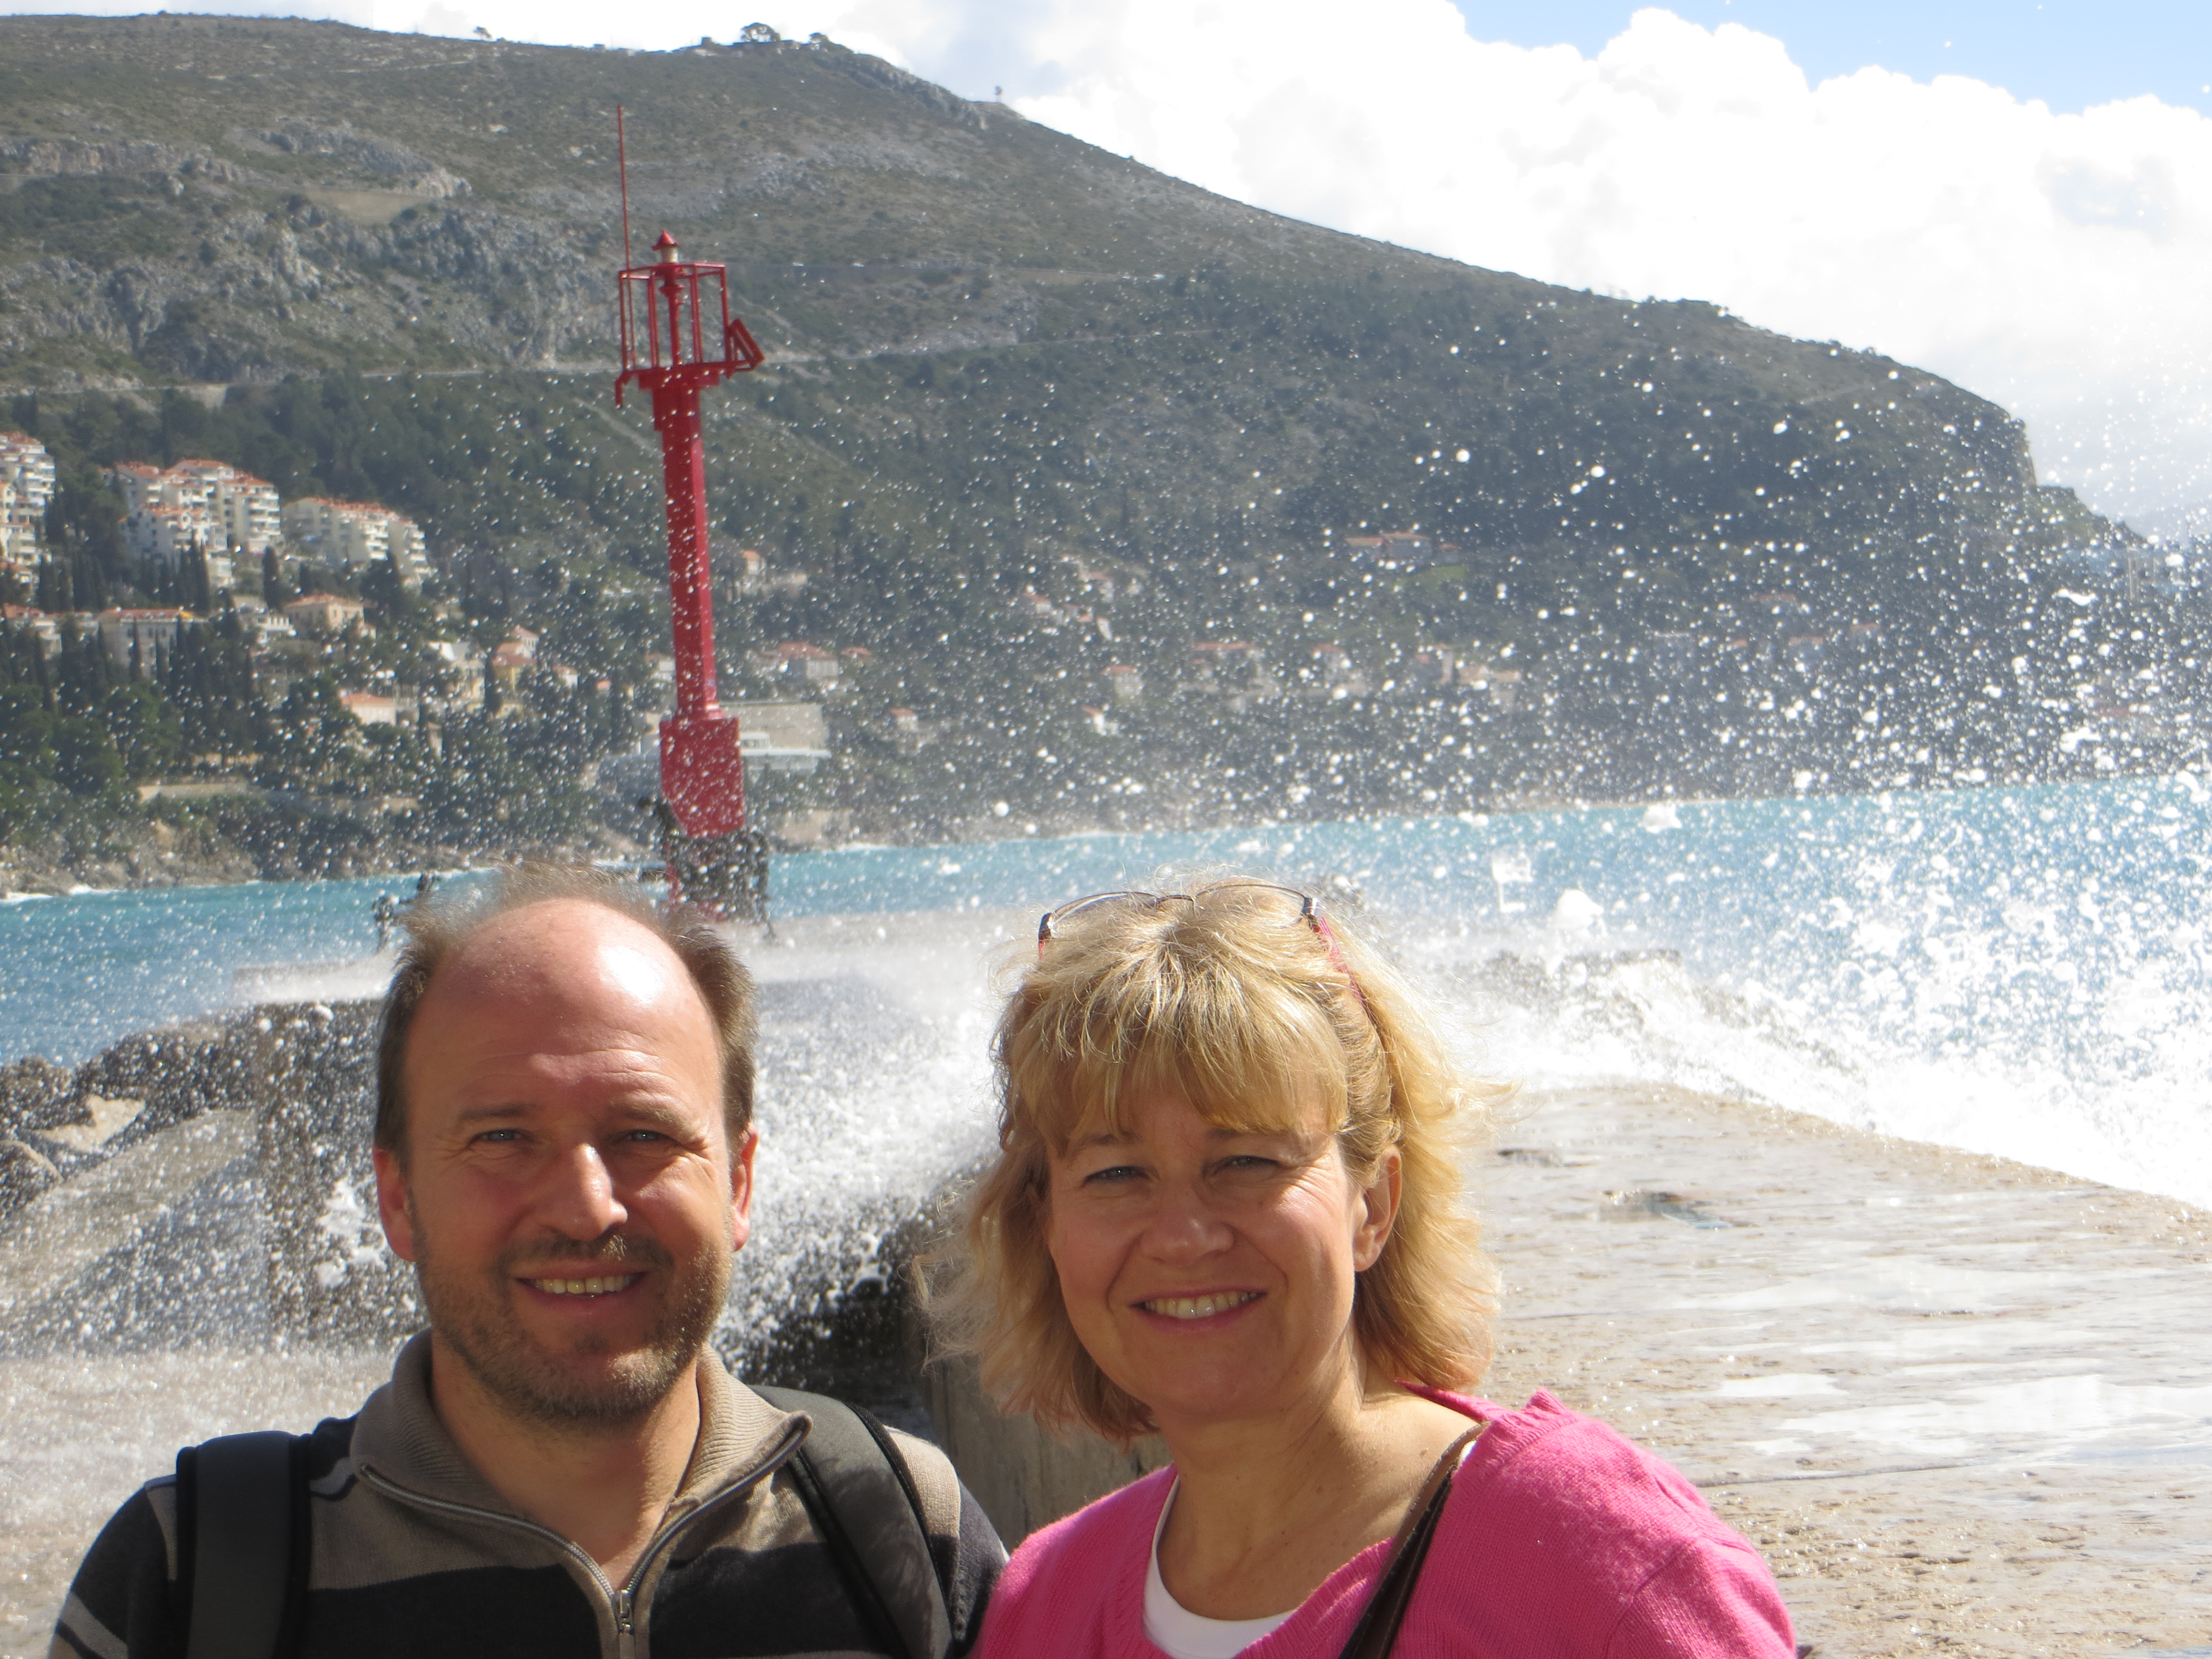
\includegraphics[width=\linewidth]{images/IMG_1216}
\captionof*{figure}{Frank i Angelika Bosch}
%\end{wrapfigure}
\end{center}
\textbf{Mihovil Dorotić} rođen je 8.8.1980. god. Akademiju likovnih umjetnosti, slikarski odjel, završava 2001. g. u klasi prof. Kokota, a 2004. g. diplomira studij klarineta u klasi prof. Pravdića  na Muzičkoj akademiji u Zagrebu. Član je HDLU-a i ULUS-a. Do sada je ostvario trinaest samostalnih izložbi, te sudjelovao na mnogim skupnim izložbama. Radi kao prof. klarineta u Zaboku.

\textit{Mihovil Dorotić, akademski slikar  
/ Grigora Viteza 11, 10432 Bregana
/ mob. 092 2710 536  
/ e-pošta: mihodoro@gmail.com}

%Sidro
\begin{center}
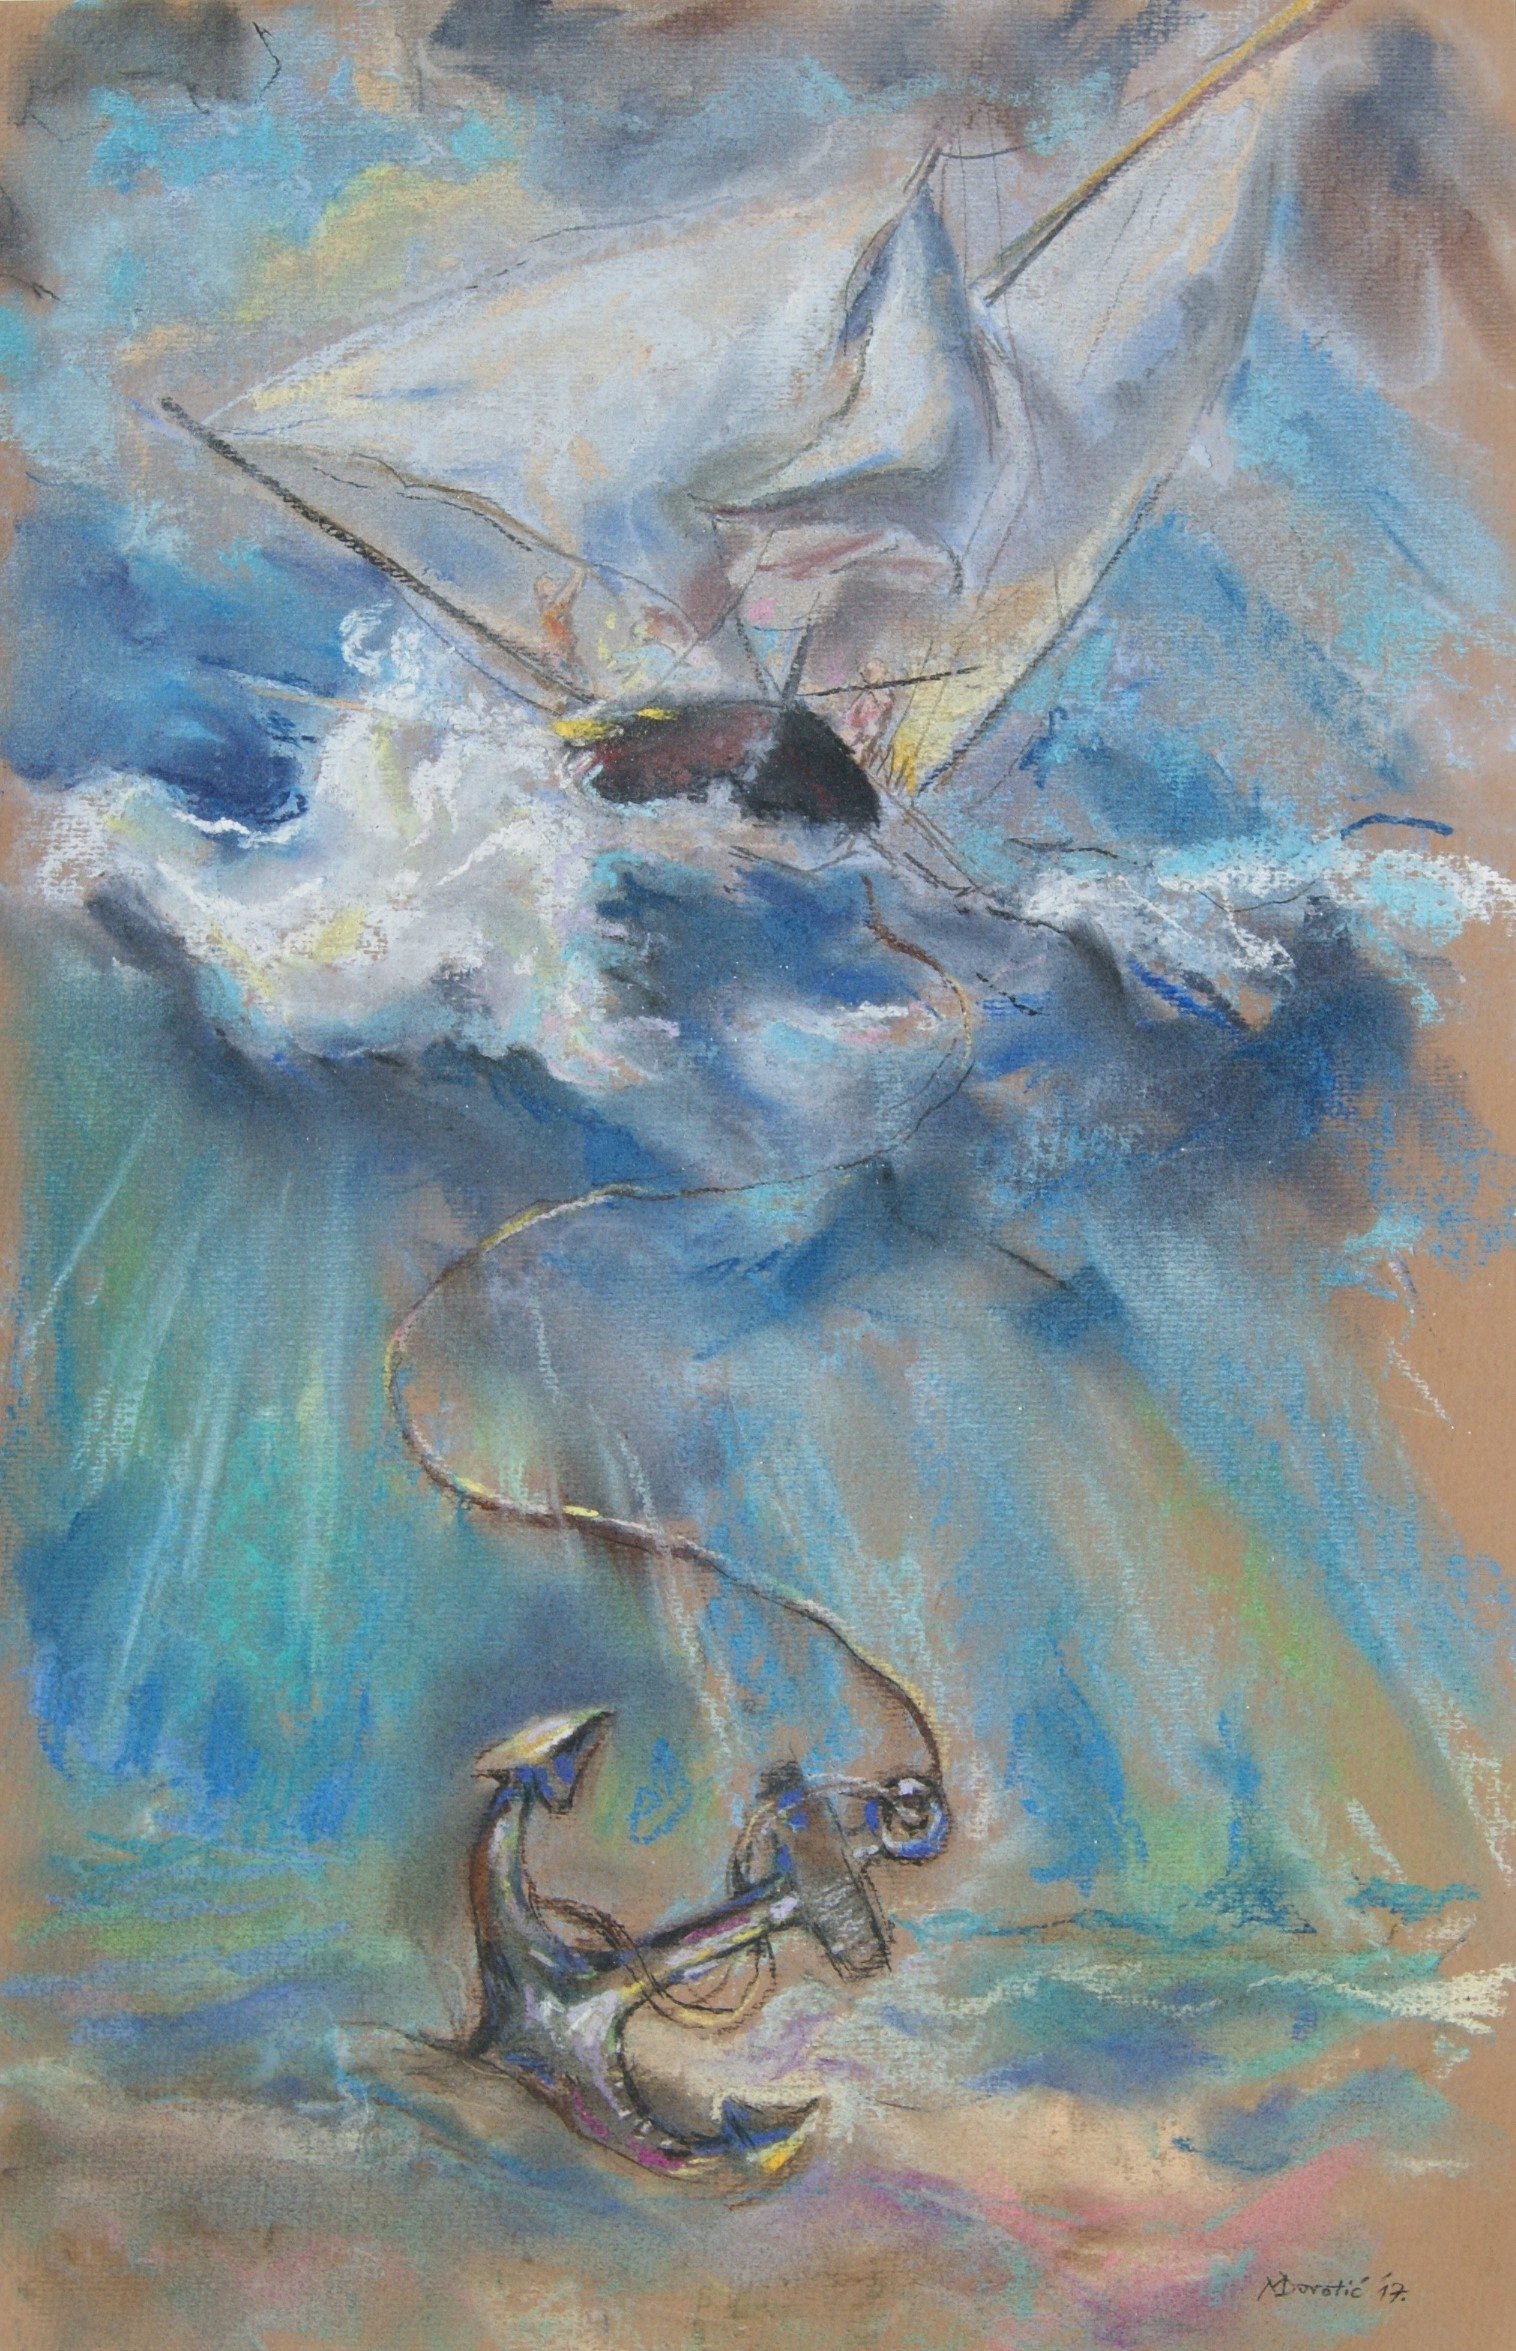
\includegraphics[width=\linewidth]{images/mihovil/a1_sidro}
\captionof*{figure}{Sidro, Mihovil Dorotić}
\end{center}

\vfill

%Mihovil Dorotić
%\begin{wrapfigure}{l}{1\linewidth}
\begin{center}
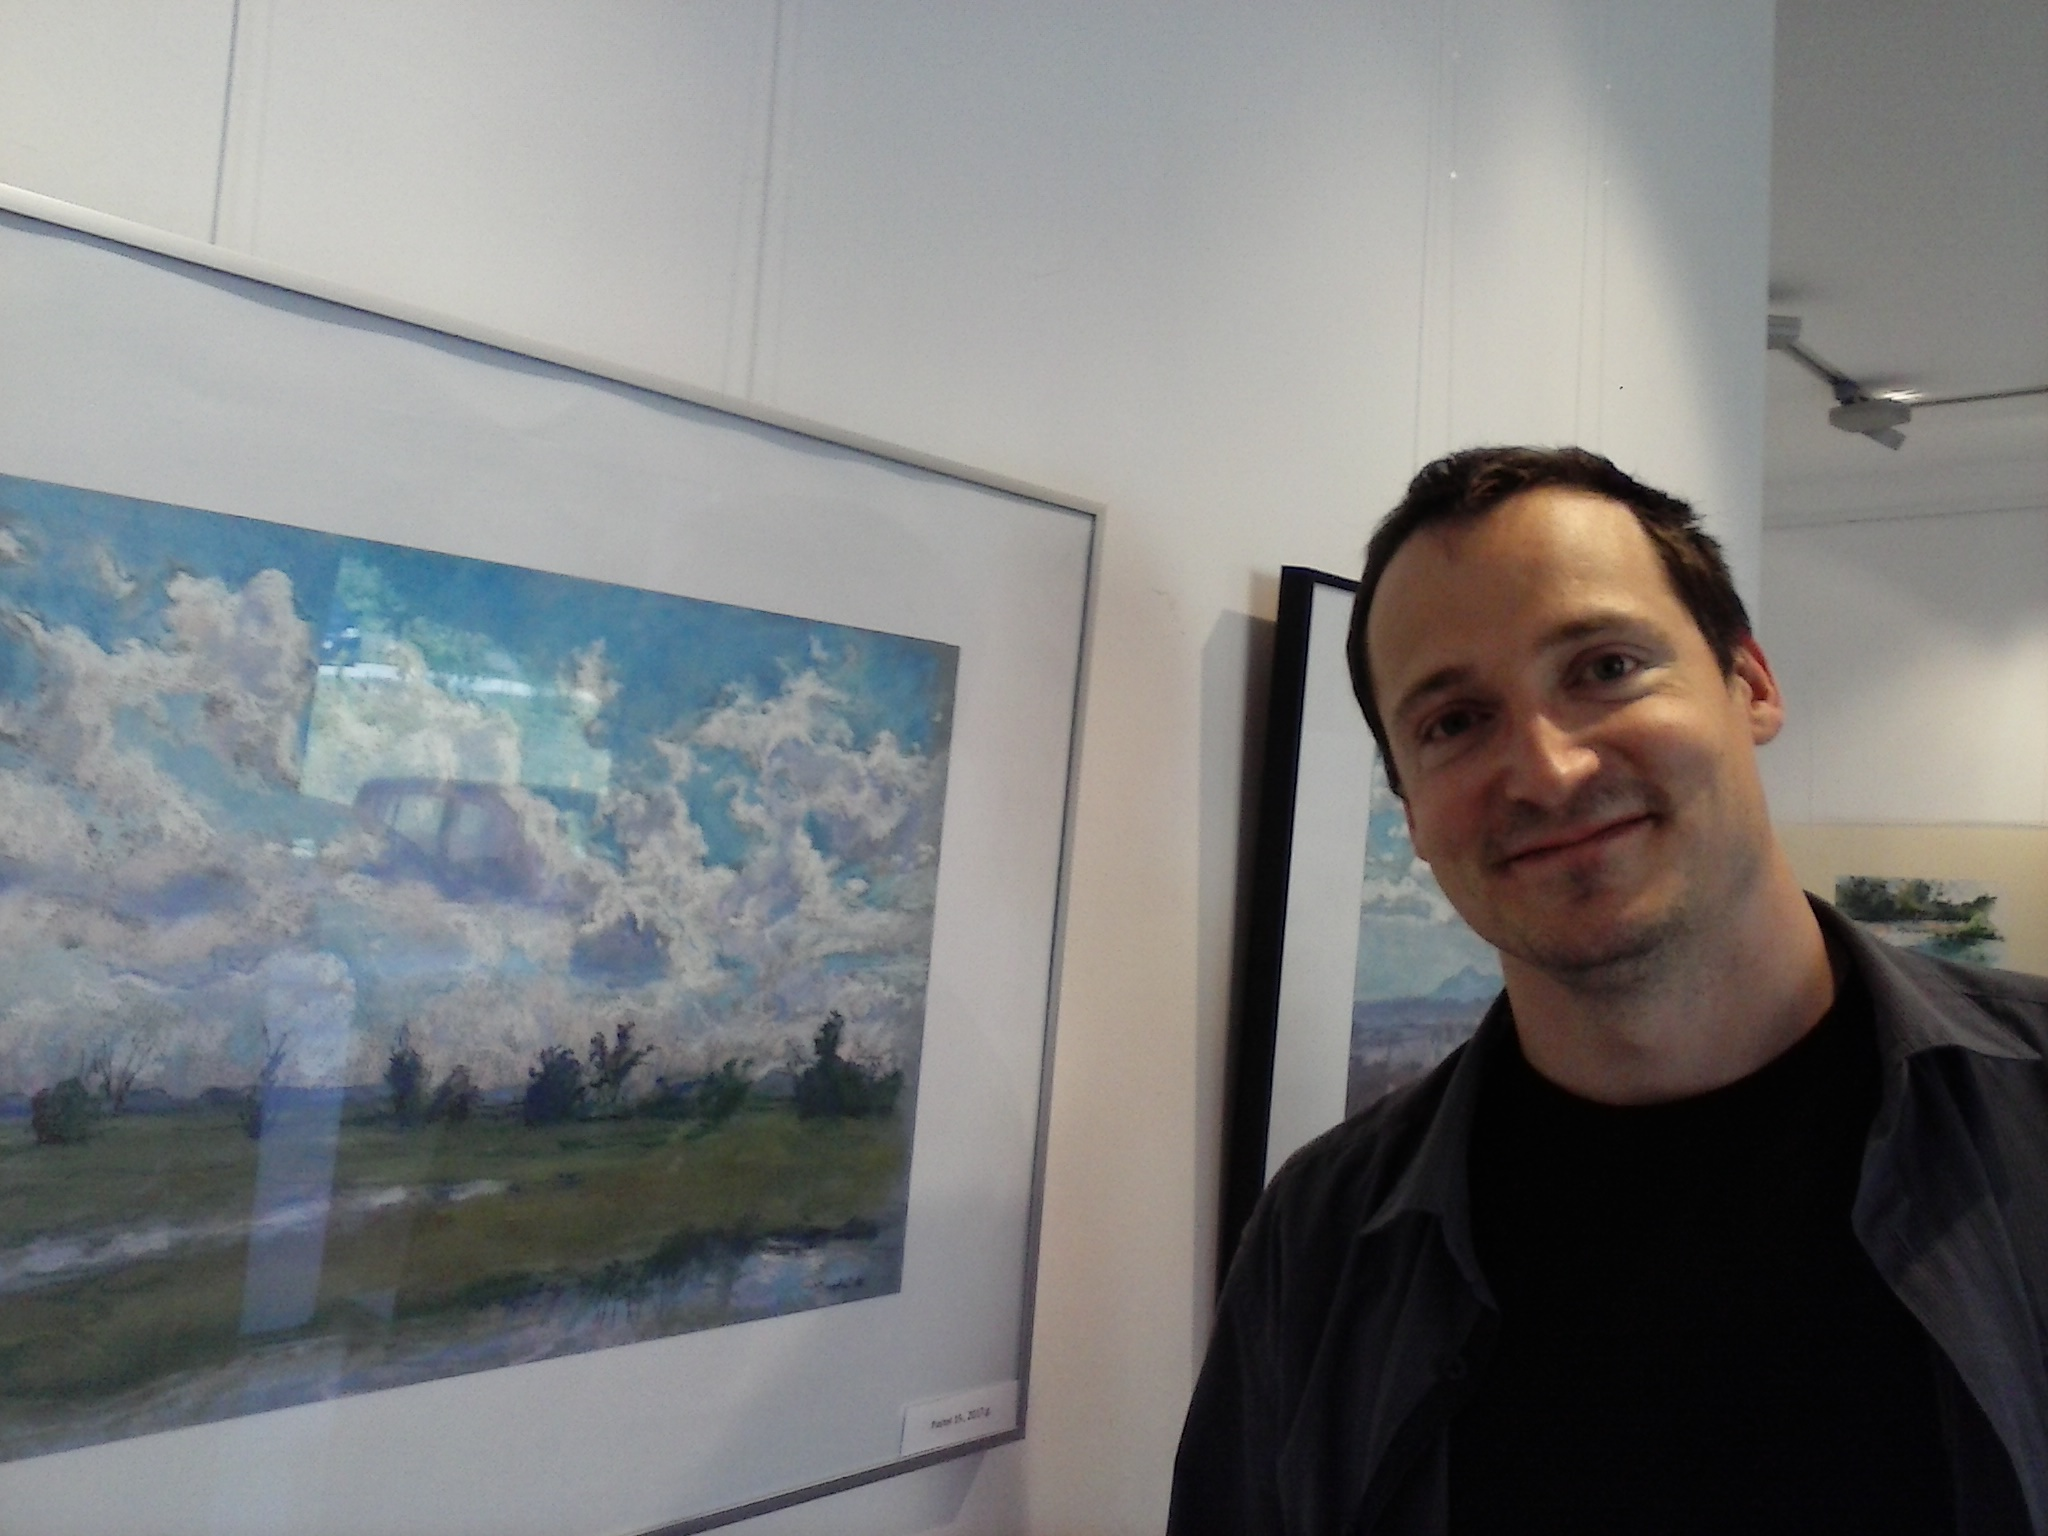
\includegraphics[width=\linewidth]{images/CAM04603}
\captionof*{figure}{Mihovil Dorotić, akademski slikar}
\end{center}

%\end{wrapfigure}


        \end{justify}
     \end{onehalfspacing}
\end{multicols}

%=========================================
%   PASTORALNI
%=========================================
\newpage
\begin{center}
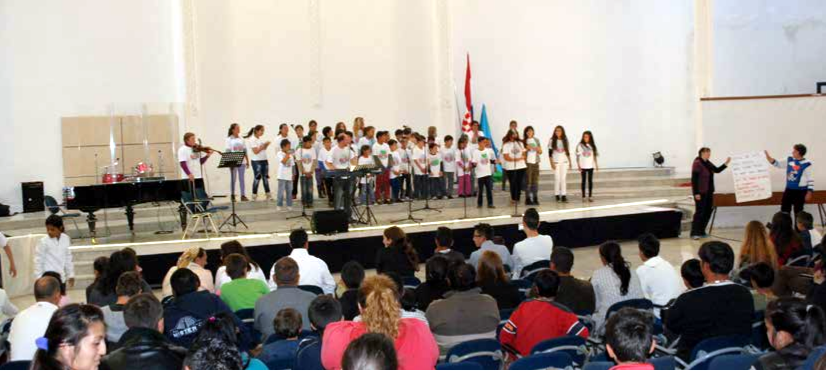
\includegraphics[width=\linewidth]{images/pastorlani}\\

\vfill

\textbf{Mjuzikids} je kršćanska interkonfesionalna udruga.
Volimo pjevati, plesati i glumiti i na taj način pokazivati koliko je velik
i dobar naš Bog, koji nam je poslao „pismo s neba„.

\vfill
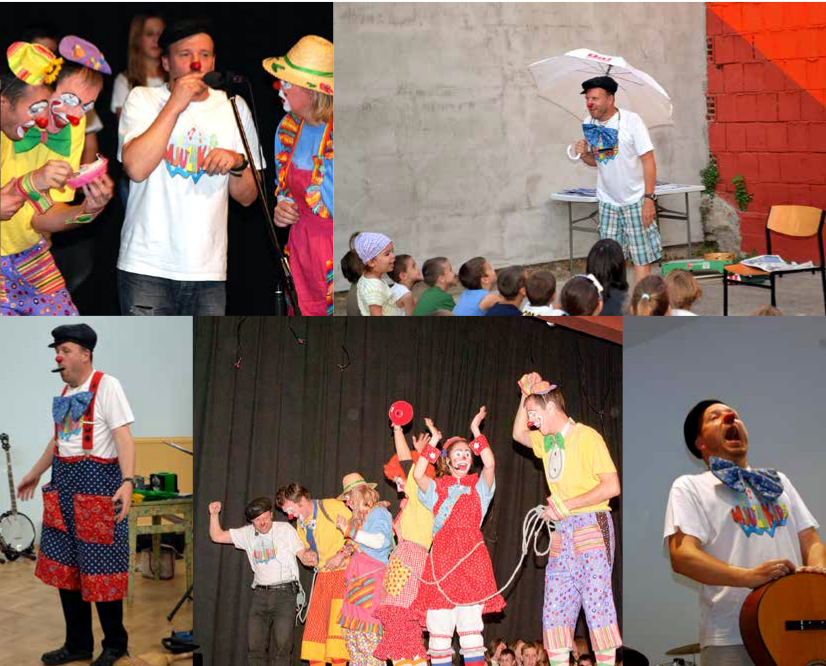
\includegraphics[width=\linewidth]{images/klauni}\\

\end{center}


%=========================================
%   PJESME
%=========================================
%pjesma 1
\newpage
\phantomsection
\begin{minipage}[b]{0.5\linewidth}
\addcontentsline{toc}{section}{\texorpdfstring{{\rednifont\doccolor1.}\hspace{\onedigitspacing}}{}SIDRO MOJE DUŠE \ttfamily(Heb 6,19)}
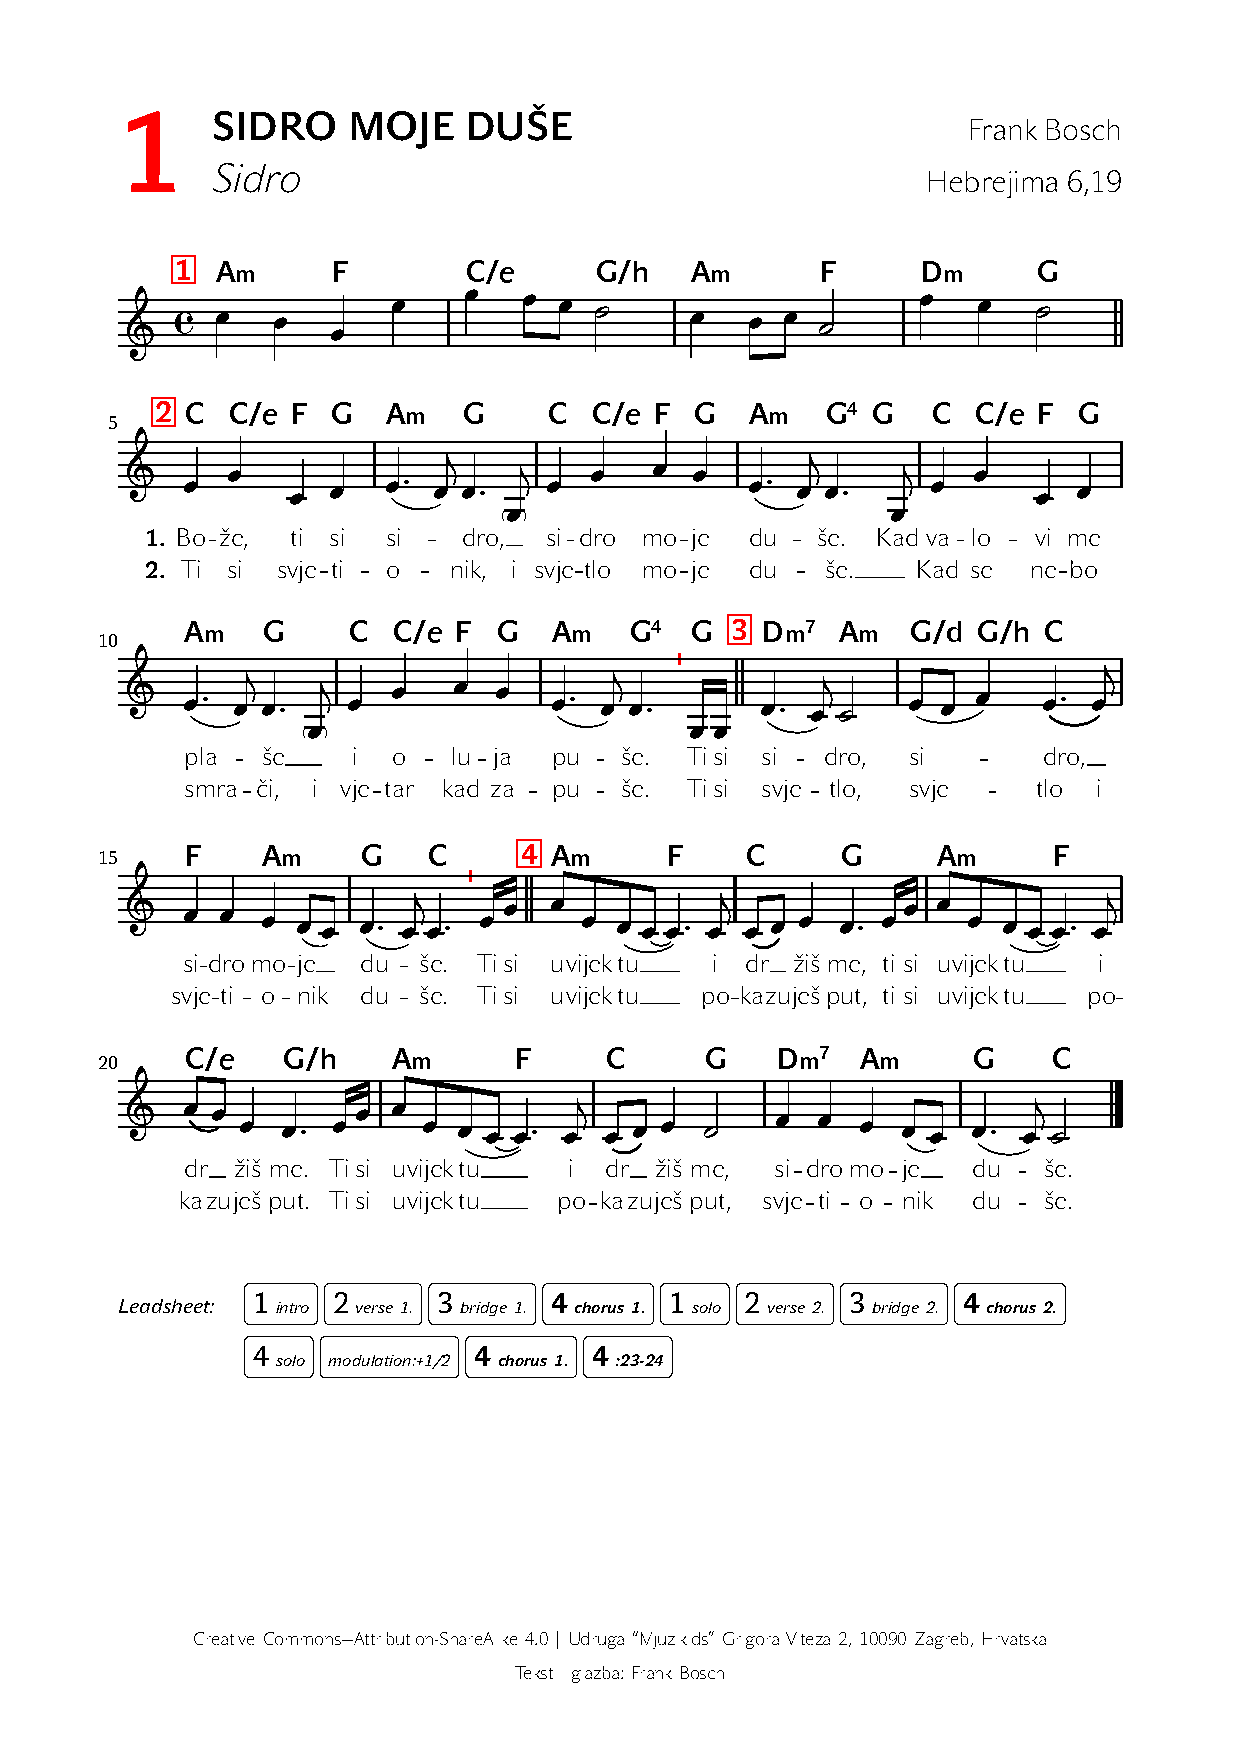
\includepdf[pages={1},noautoscale]{lilypond/hr/src/01_sidro_moje_duse.pdf}
\end{minipage}

\newpage
\begin{center}
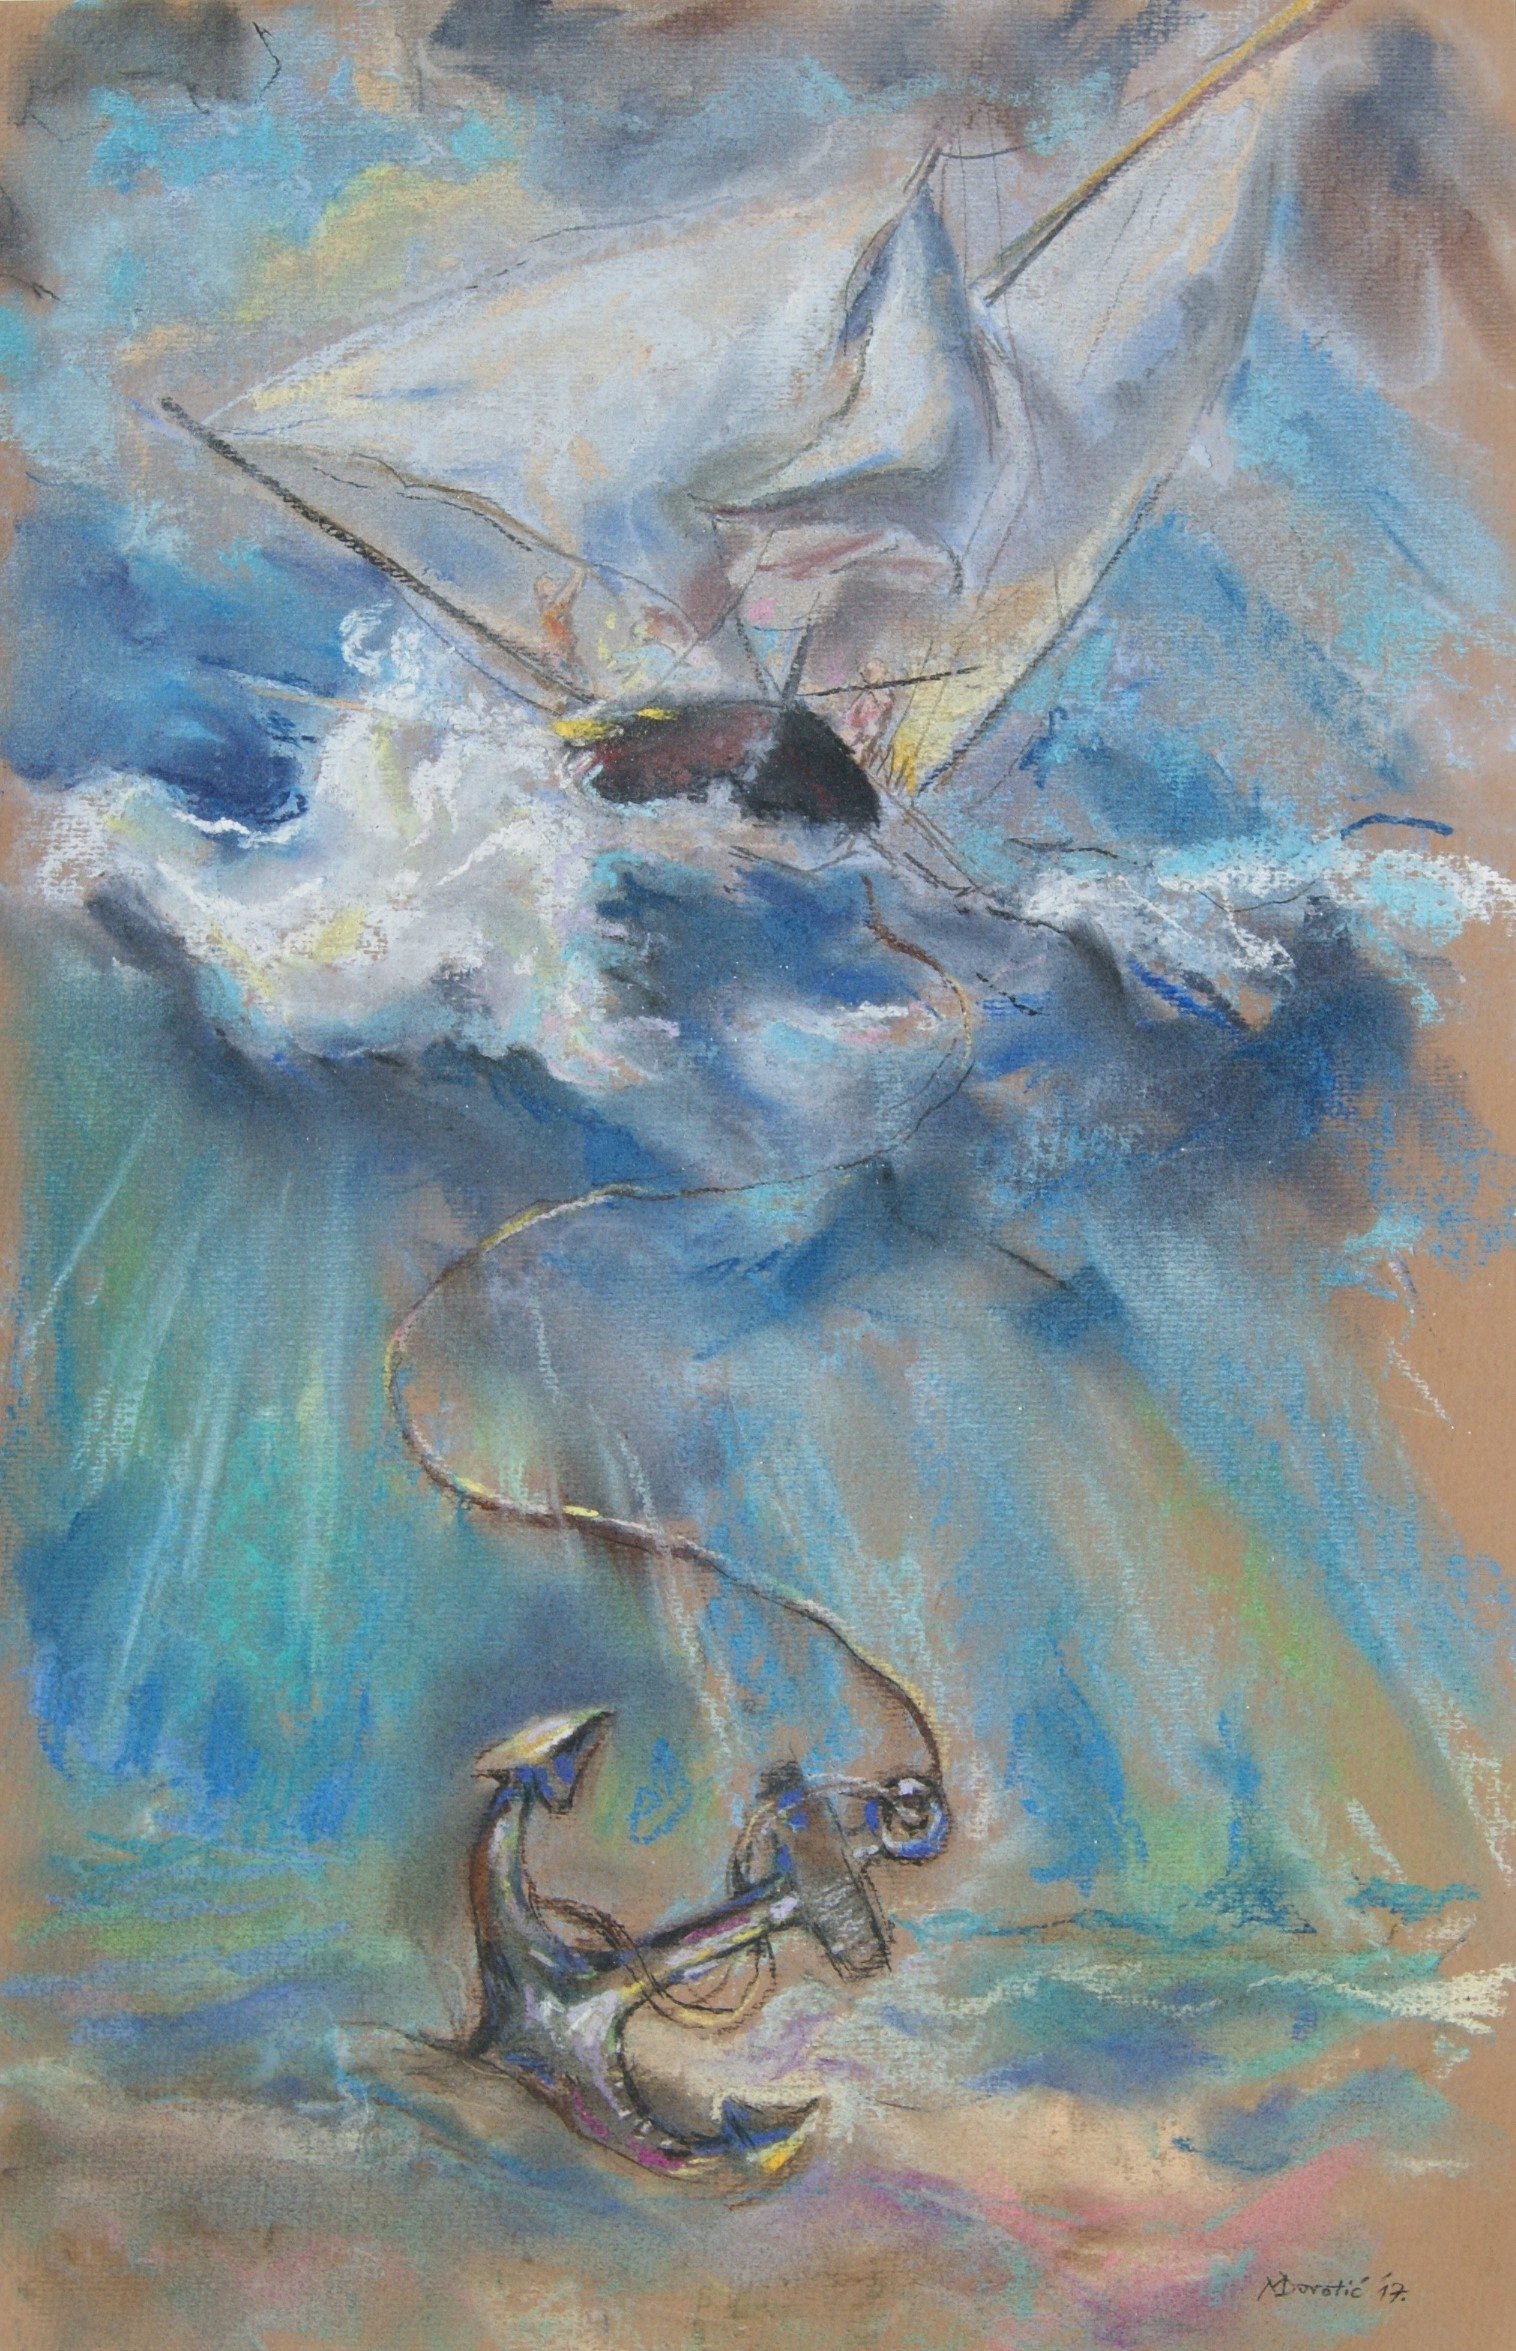
\includegraphics[width=0.9\linewidth]{images/mihovil/a1_sidro}
\end{center}

%pjesma 2
\newpage
\phantomsection
\begin{minipage}[b]{0.5\linewidth}
\addcontentsline{toc}{section}{\texorpdfstring{{\rednifont\doccolor2.}\hspace{\onedigitspacing}}{}LJUBAV JE STRPLJIVA \ttfamily(1 Kor 13,4-5.13)}
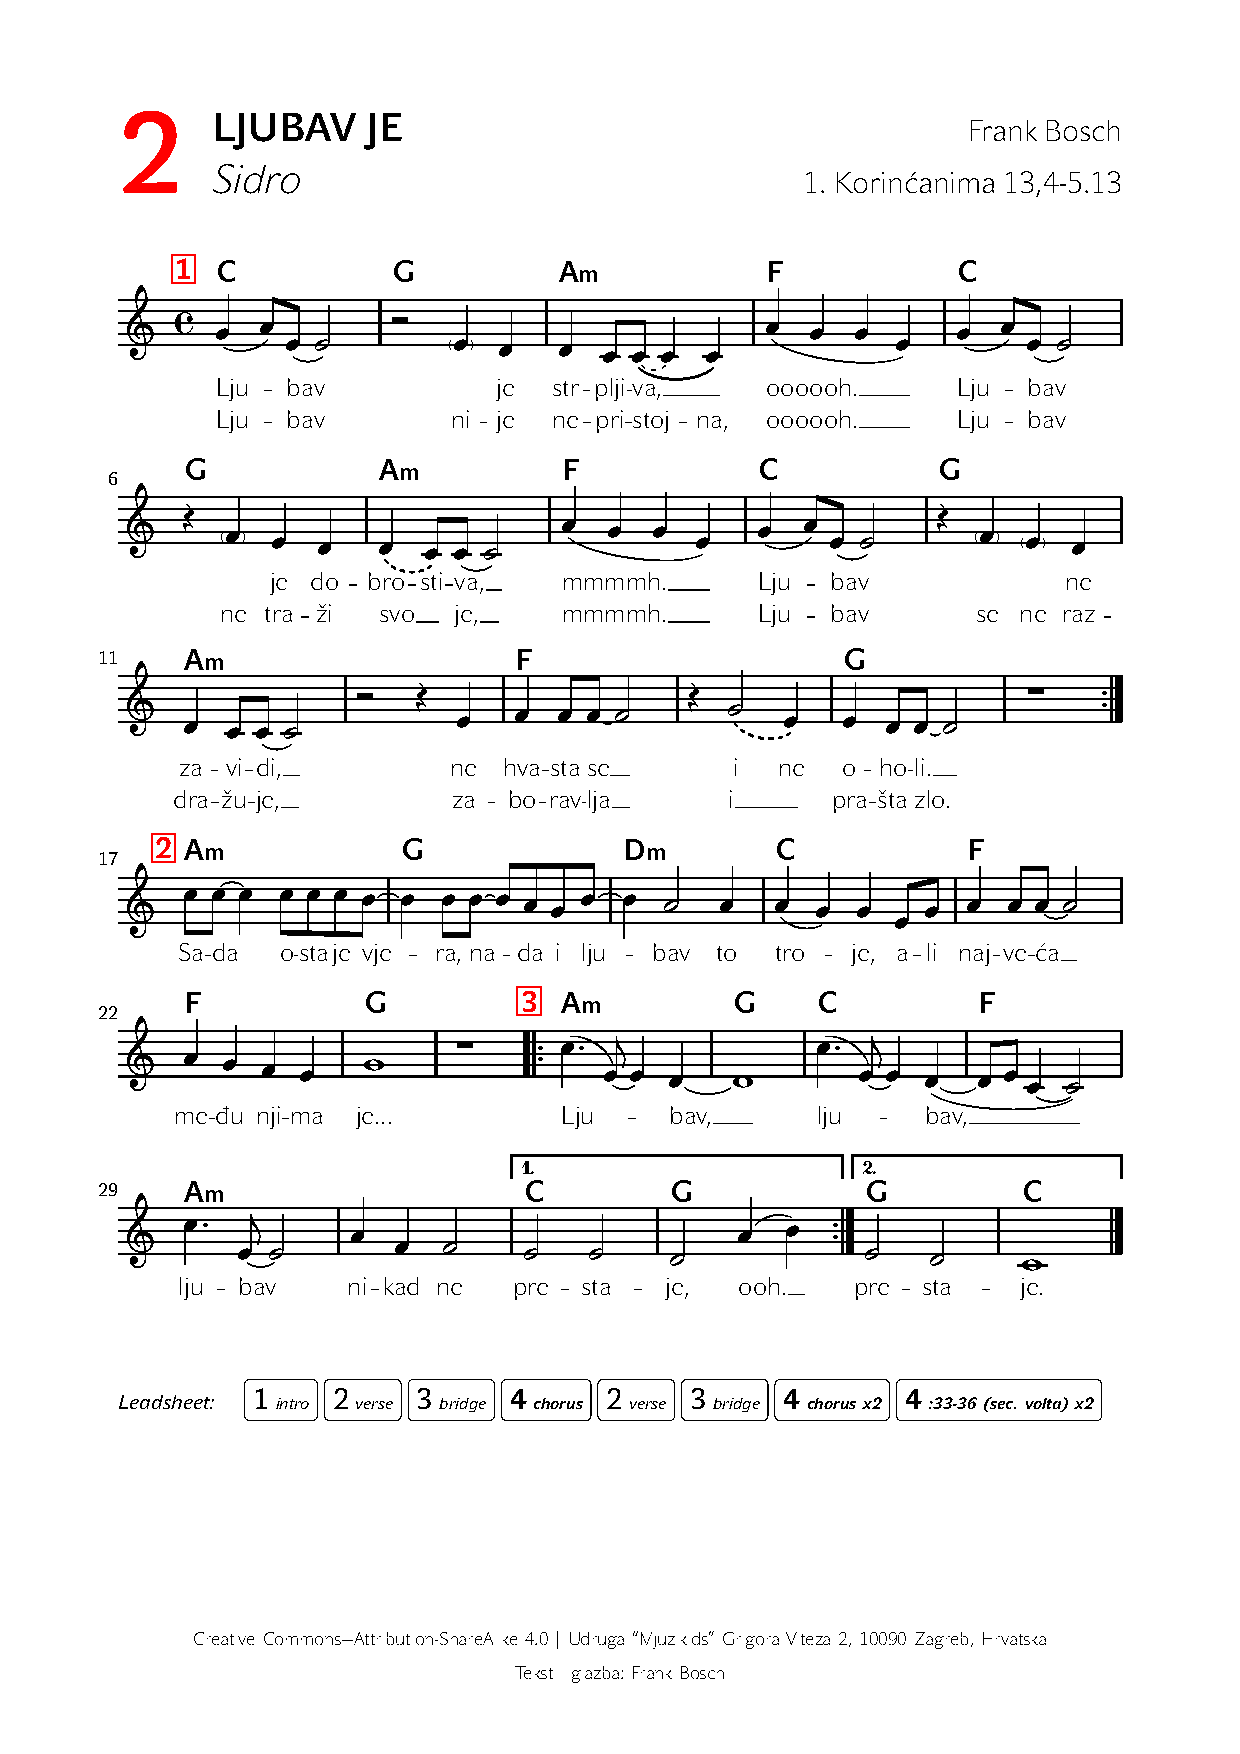
\includepdf[pages={1},noautoscale]{lilypond/hr/src/02_ljubav_je_strpljiva.pdf}
\end{minipage}

\newpage
\begin{center}
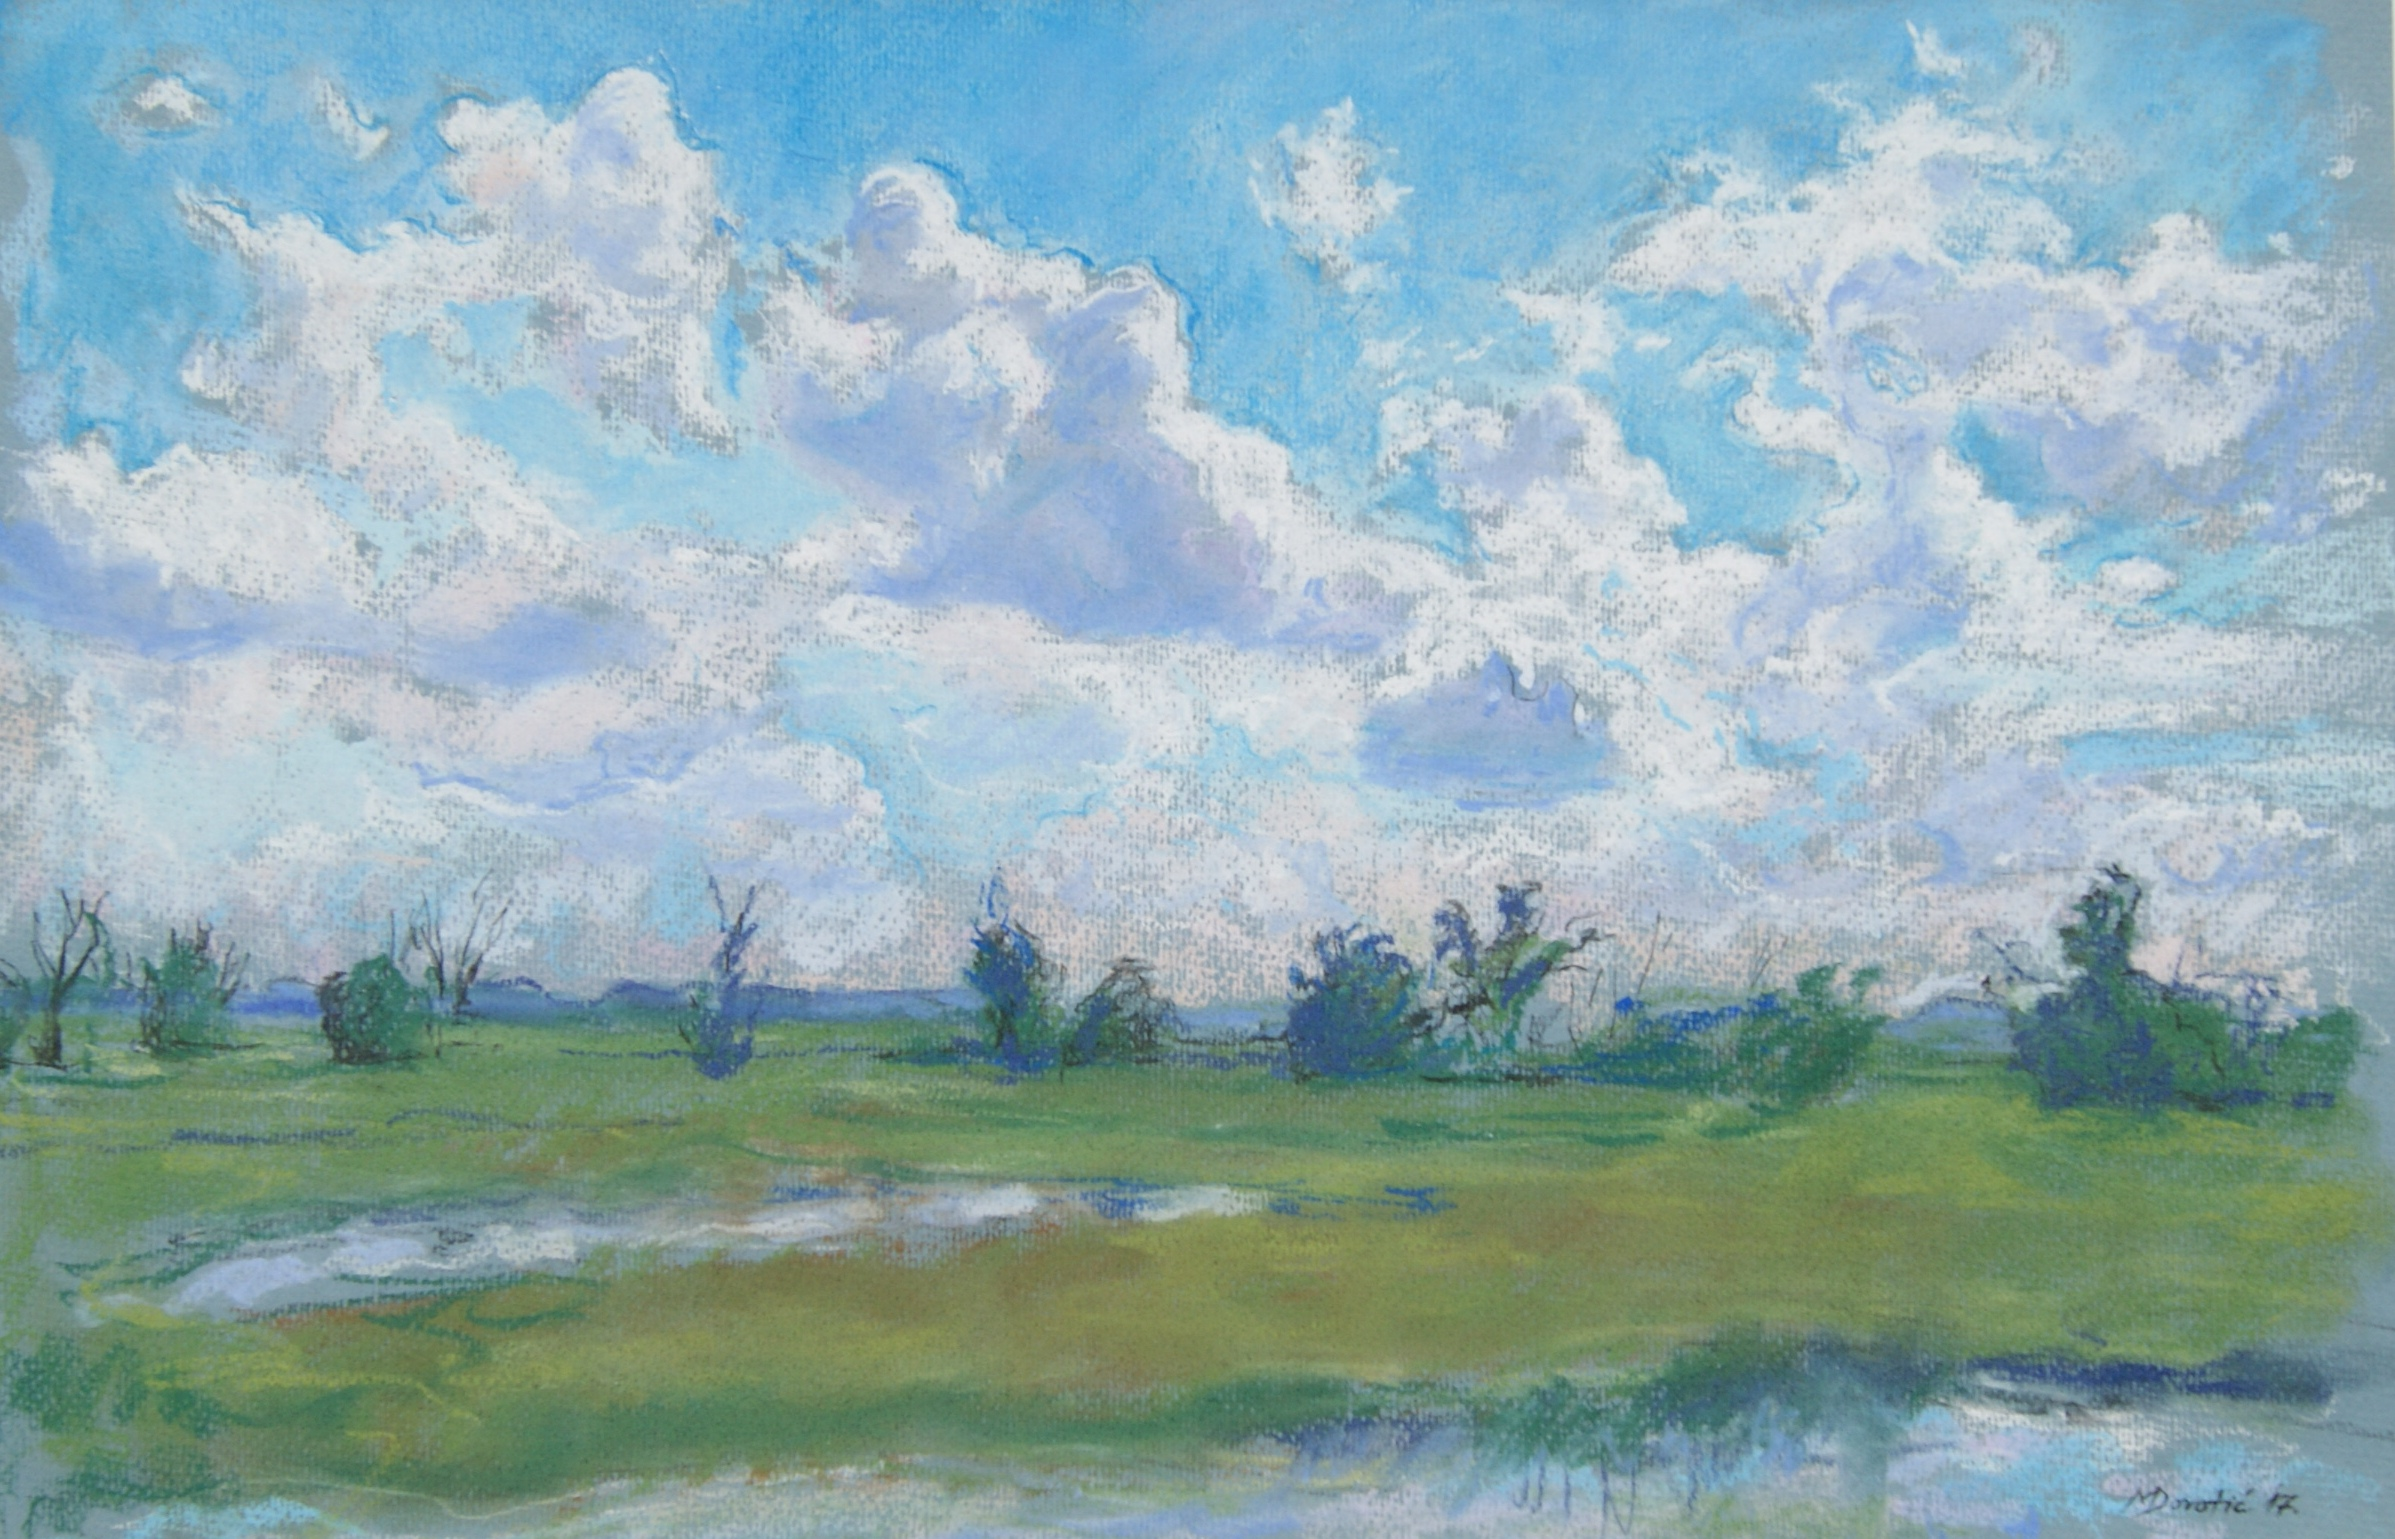
\includegraphics[width=\linewidth]{images/mihovil/b2_ljubav}\\
\vspace*{1cm}
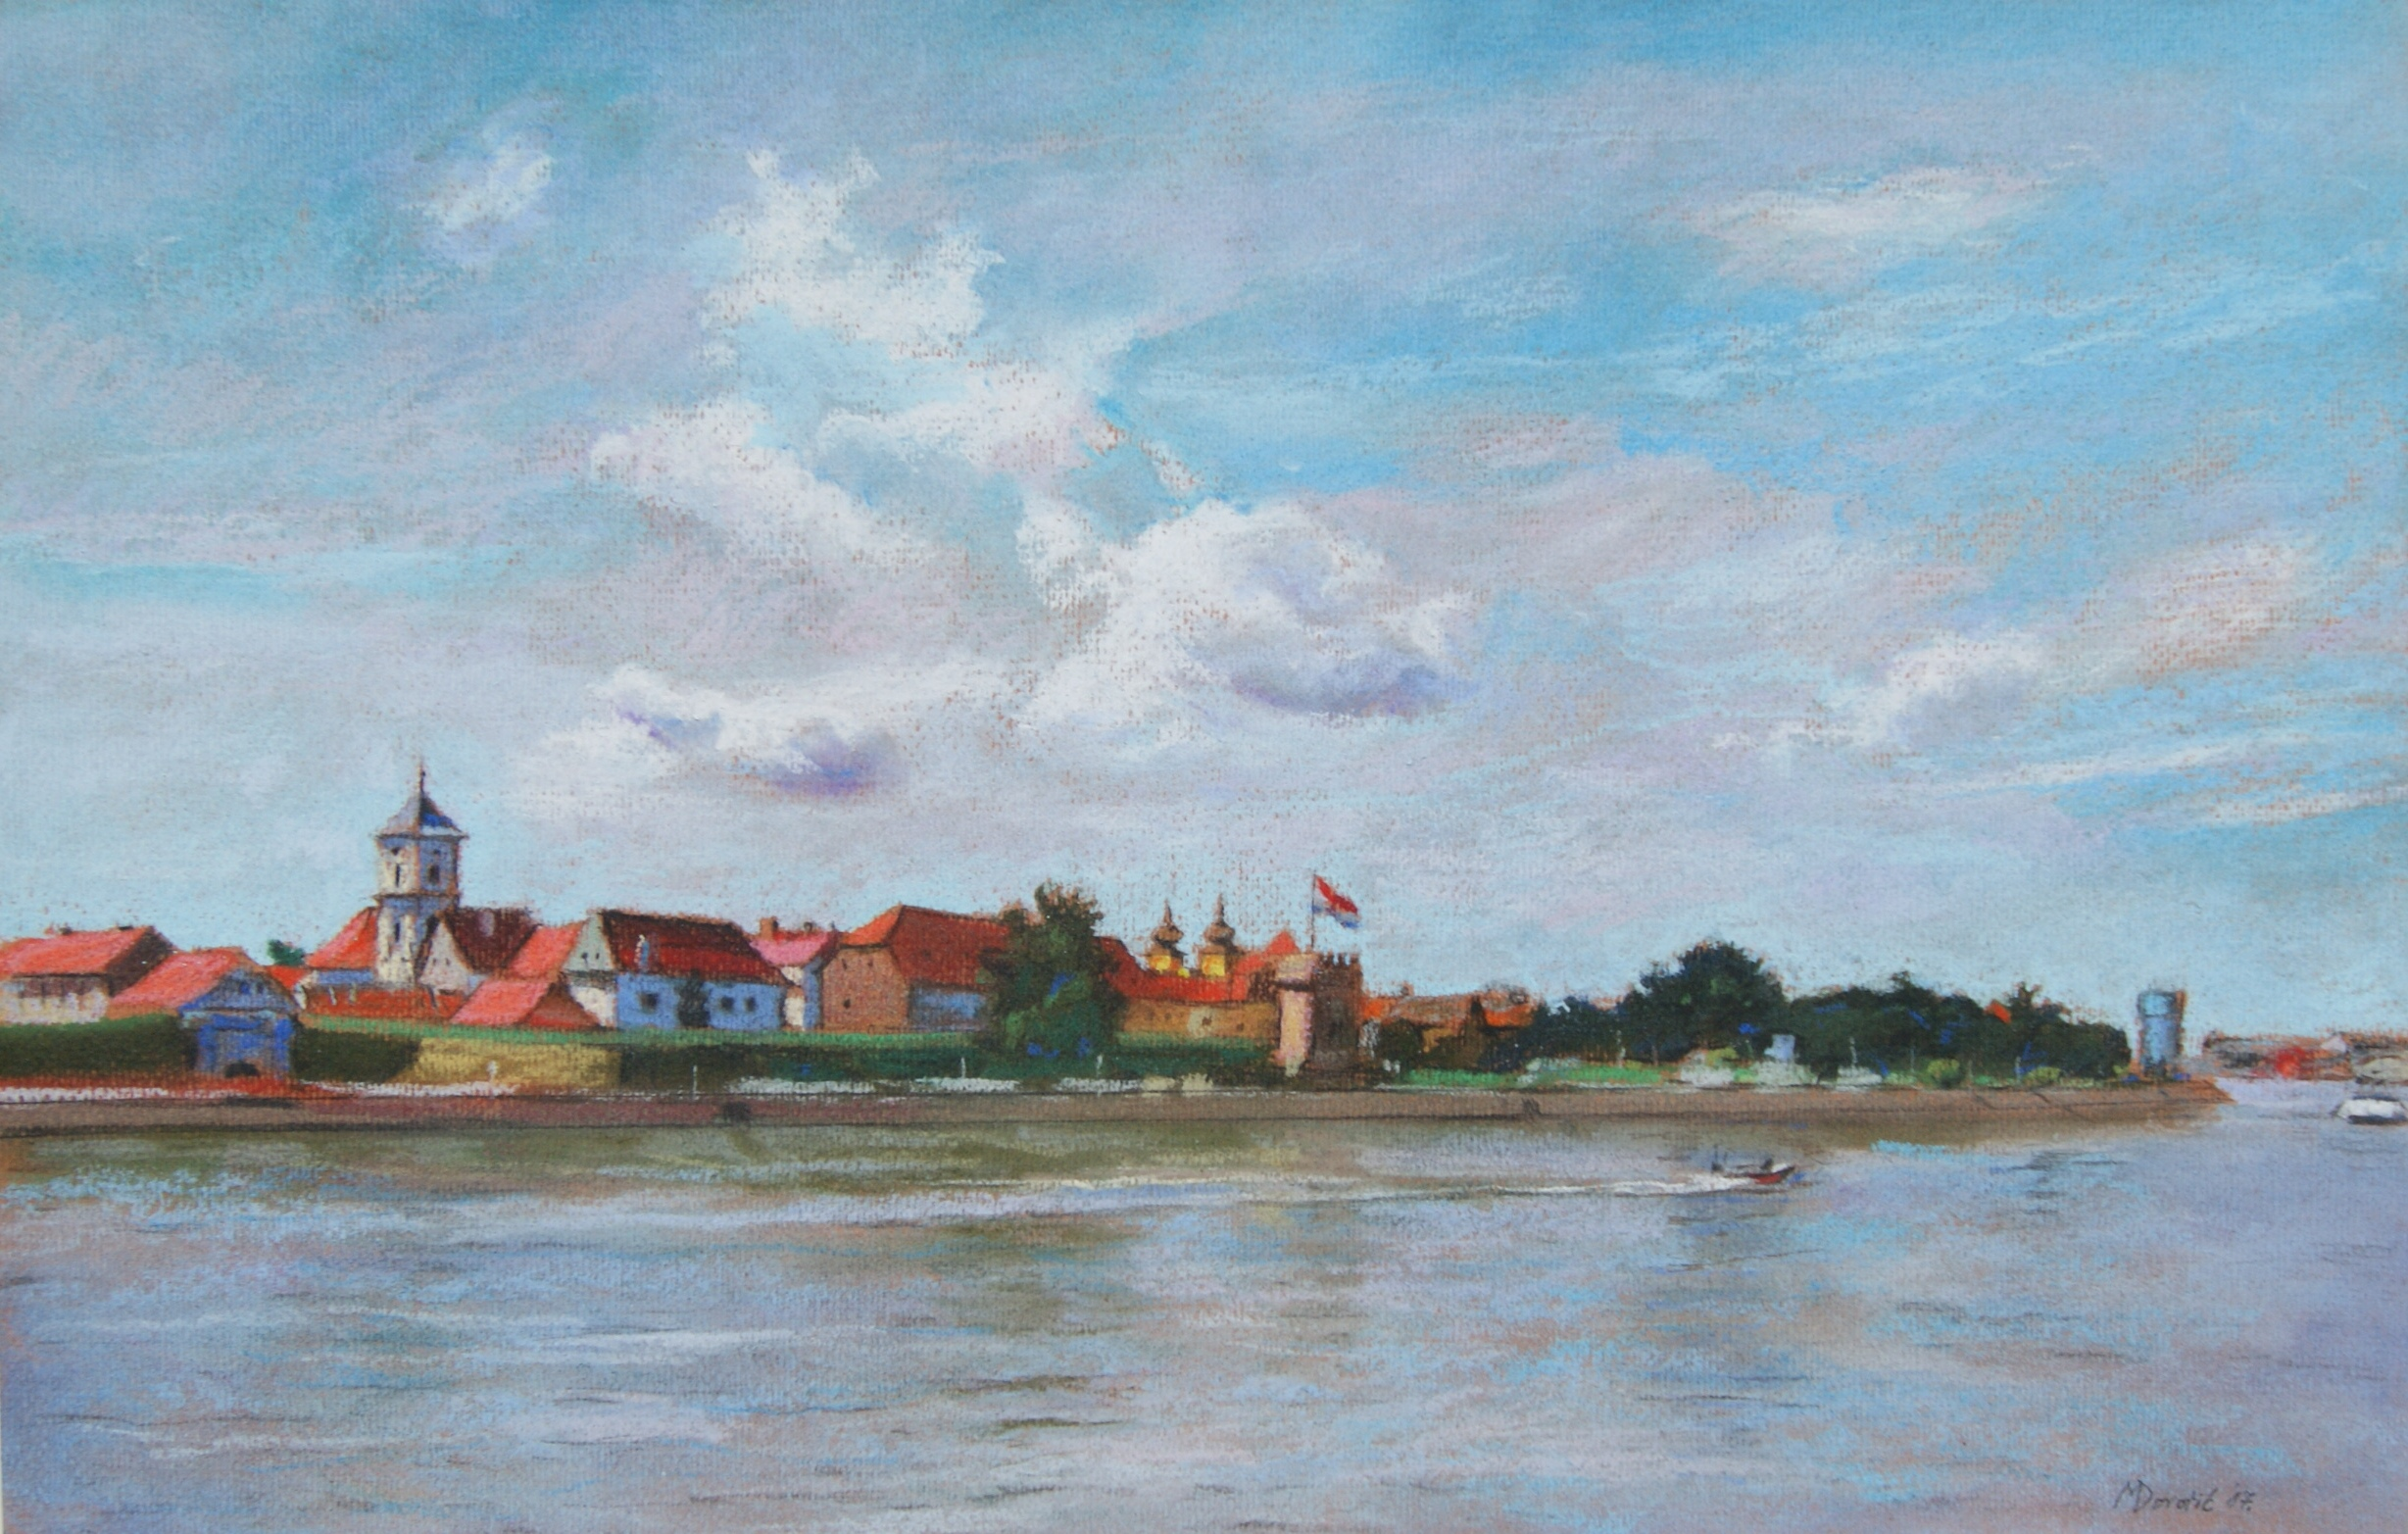
\includegraphics[width=\linewidth]{images/mihovil/pejza_10}
\end{center}

%pjesma 3
\newpage
\phantomsection
\begin{minipage}[b]{0.5\linewidth}
\addcontentsline{toc}{section}{\texorpdfstring{{\rednifont\doccolor3.}\hspace{\onedigitspacing}}{}PLANOVI MIRA \ttfamily(Jr 29,11)}
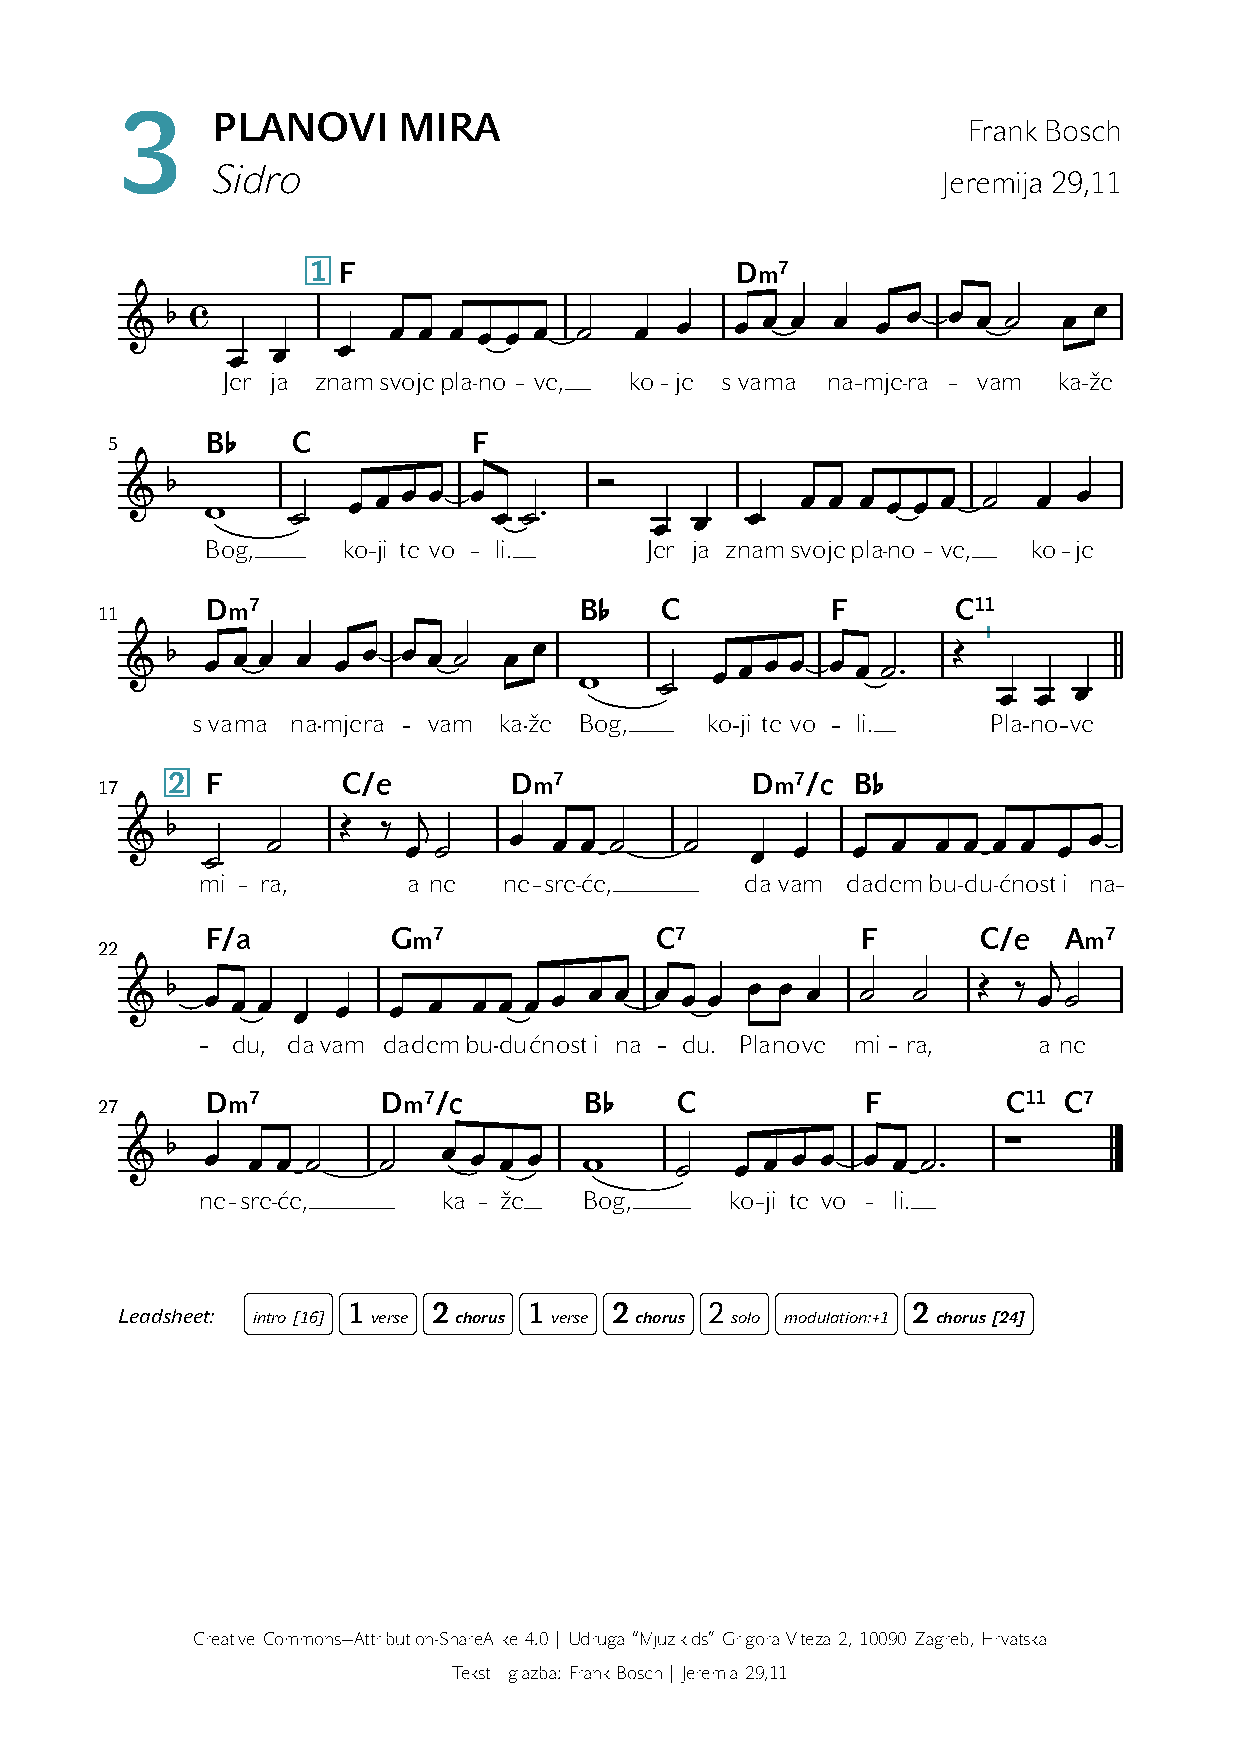
\includepdf[pages={1},noautoscale]{lilypond/hr/src/03_planove_mira.pdf}
\end{minipage}

% \newpage
% \begin{center}
% 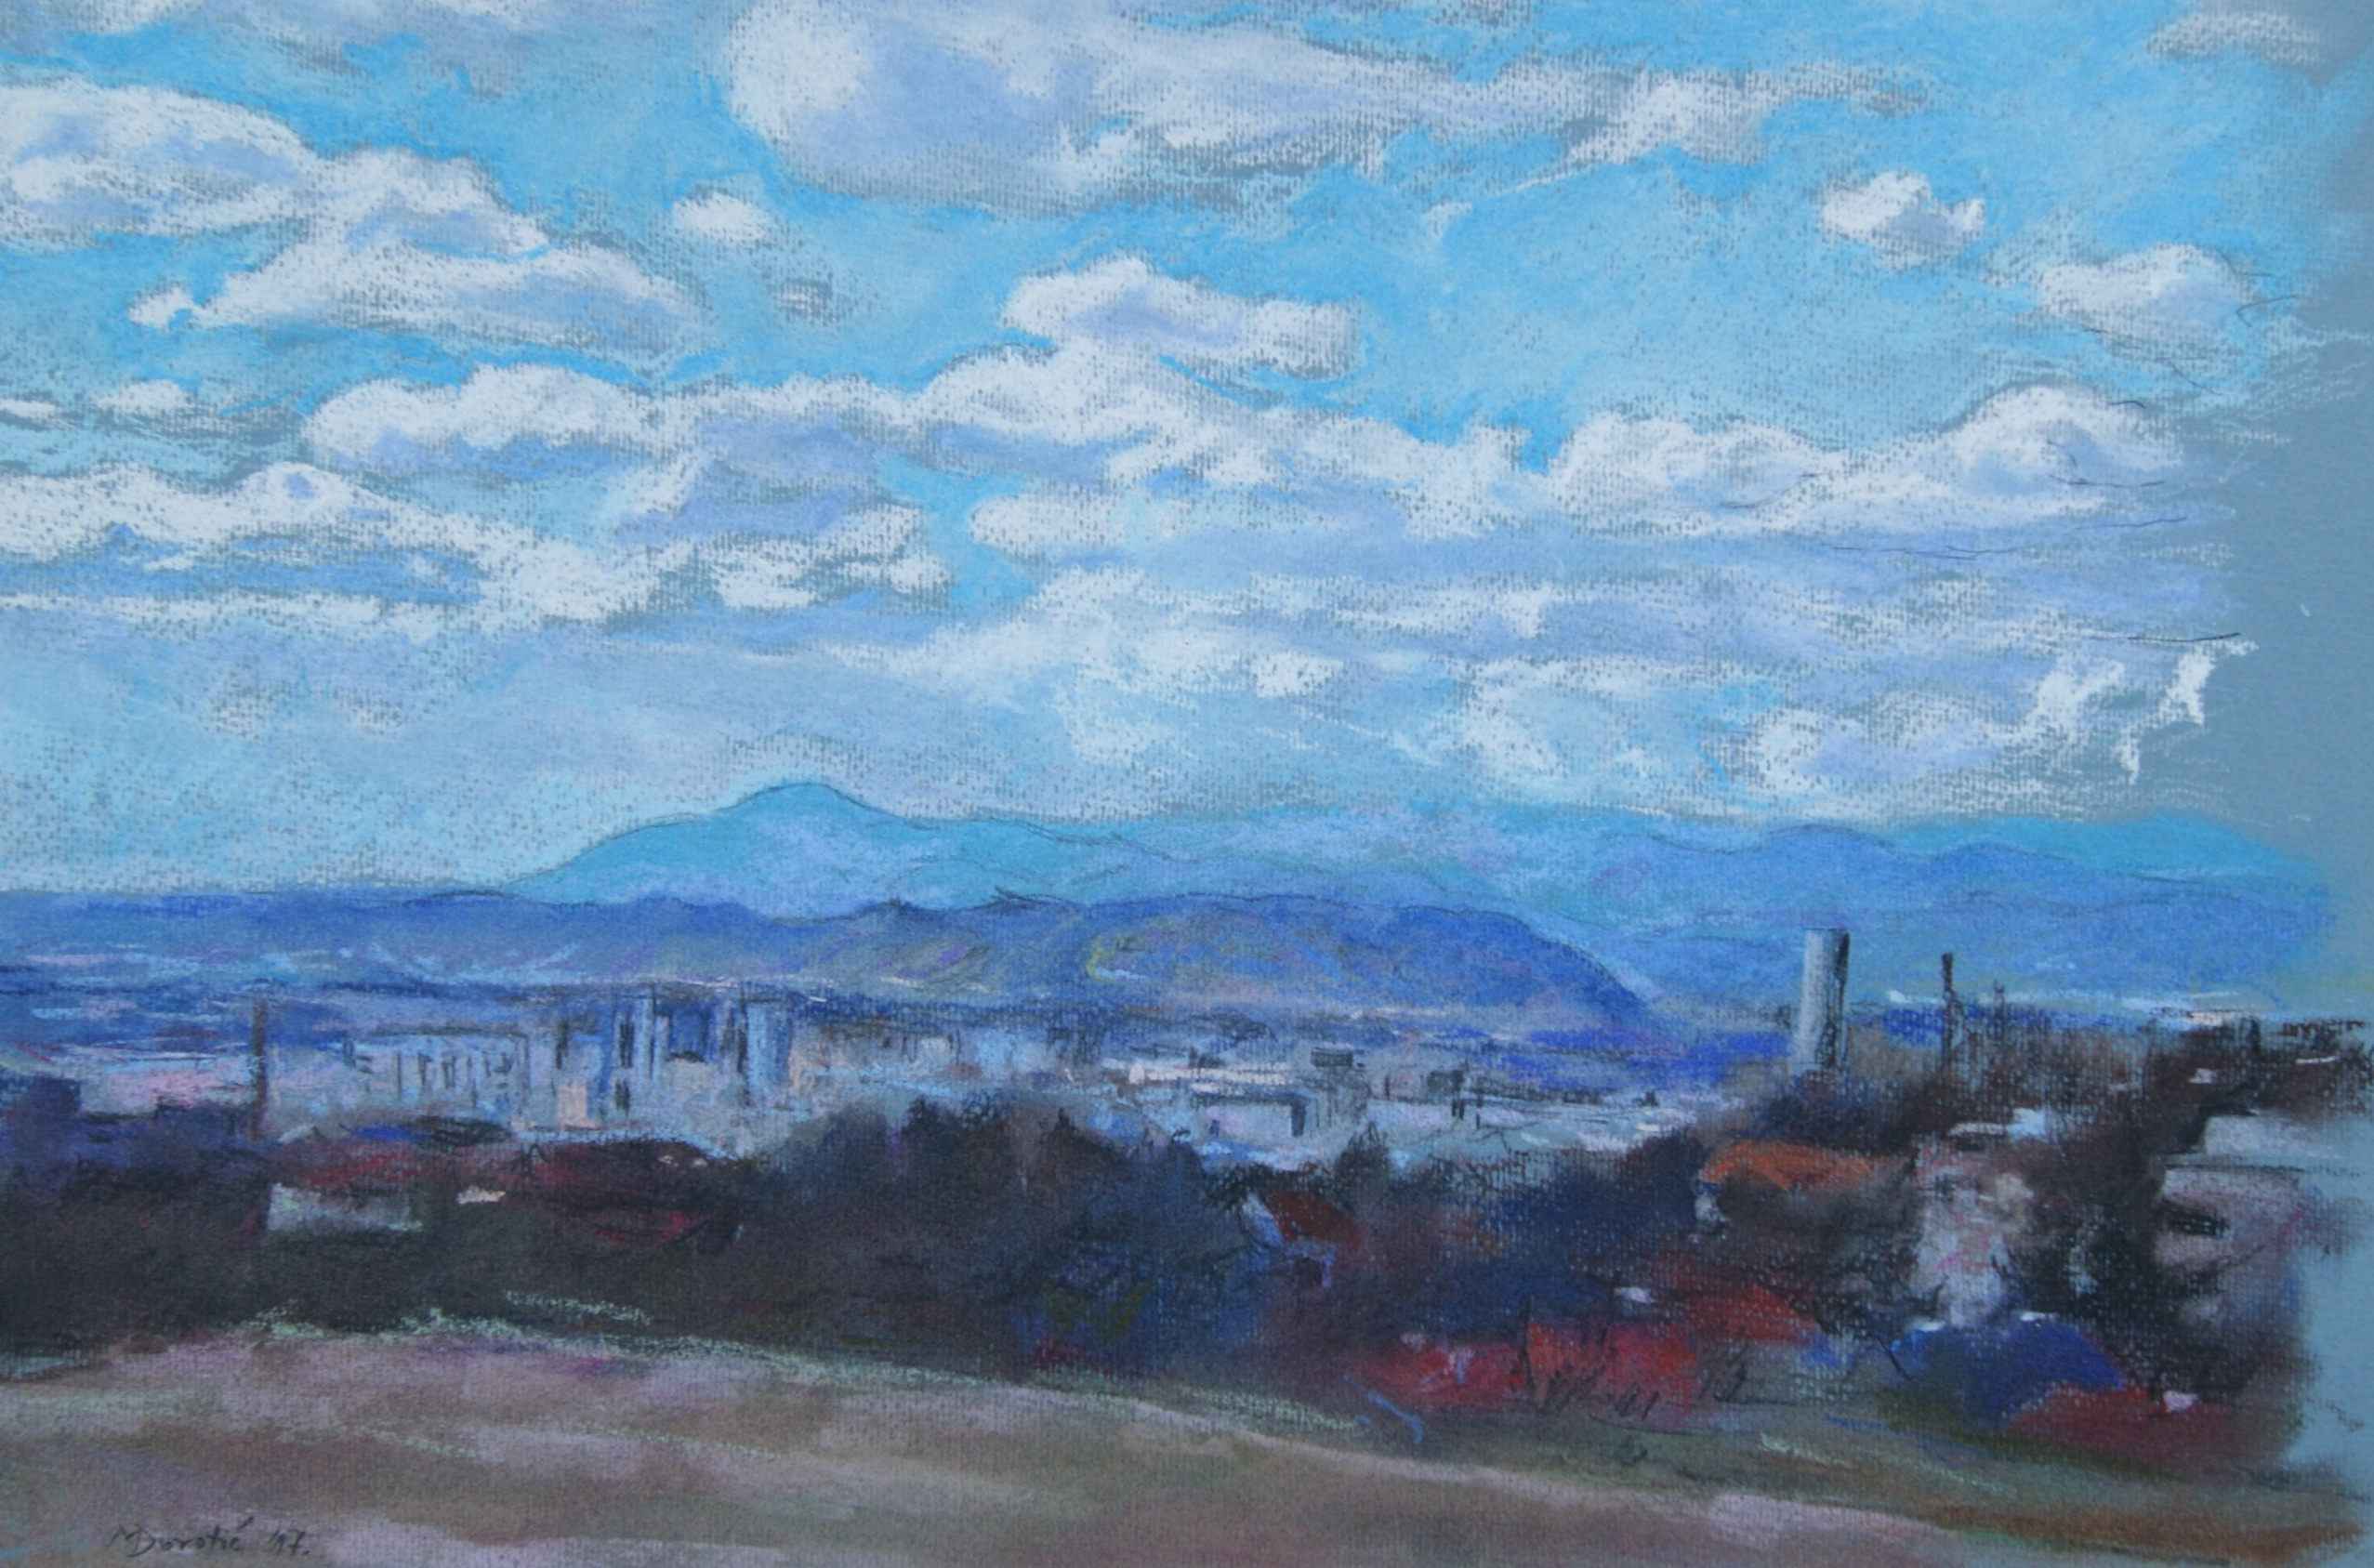
\includegraphics[width=\linewidth]{images/mihovil/c3_planovemira}

% \vspace*{1mm}
% \begin{center}

% 	\Large{\parbox{\linewidth}{
% 		\begin{center}
% 		{\Large
% 		\texttt{
% 			\textit{"'Jer ja znam svoje naume koje s vama namjeravam' – riječ je Jahvina – 'naume mira, a ne nesreće: da vam dadnem budućnost i nadu.'"}
% 			}
% 		}
% 		\end{center}
% 		\begin{center}
% 		{\Large
% 			\texttt{{\textemdash Jeremija 29,11}}
% 		}
% 		\end{center}
% 	}
% }
% \end{center}

% \end{center}


%pjesma 4
\newpage
\phantomsection
\addcontentsline{toc}{section}{\texorpdfstring{{\rednifont\doccolor4.}\hspace{\onedigitspacing}}{}JA I MOJ DOM \ttfamily(Jš 24,15)}
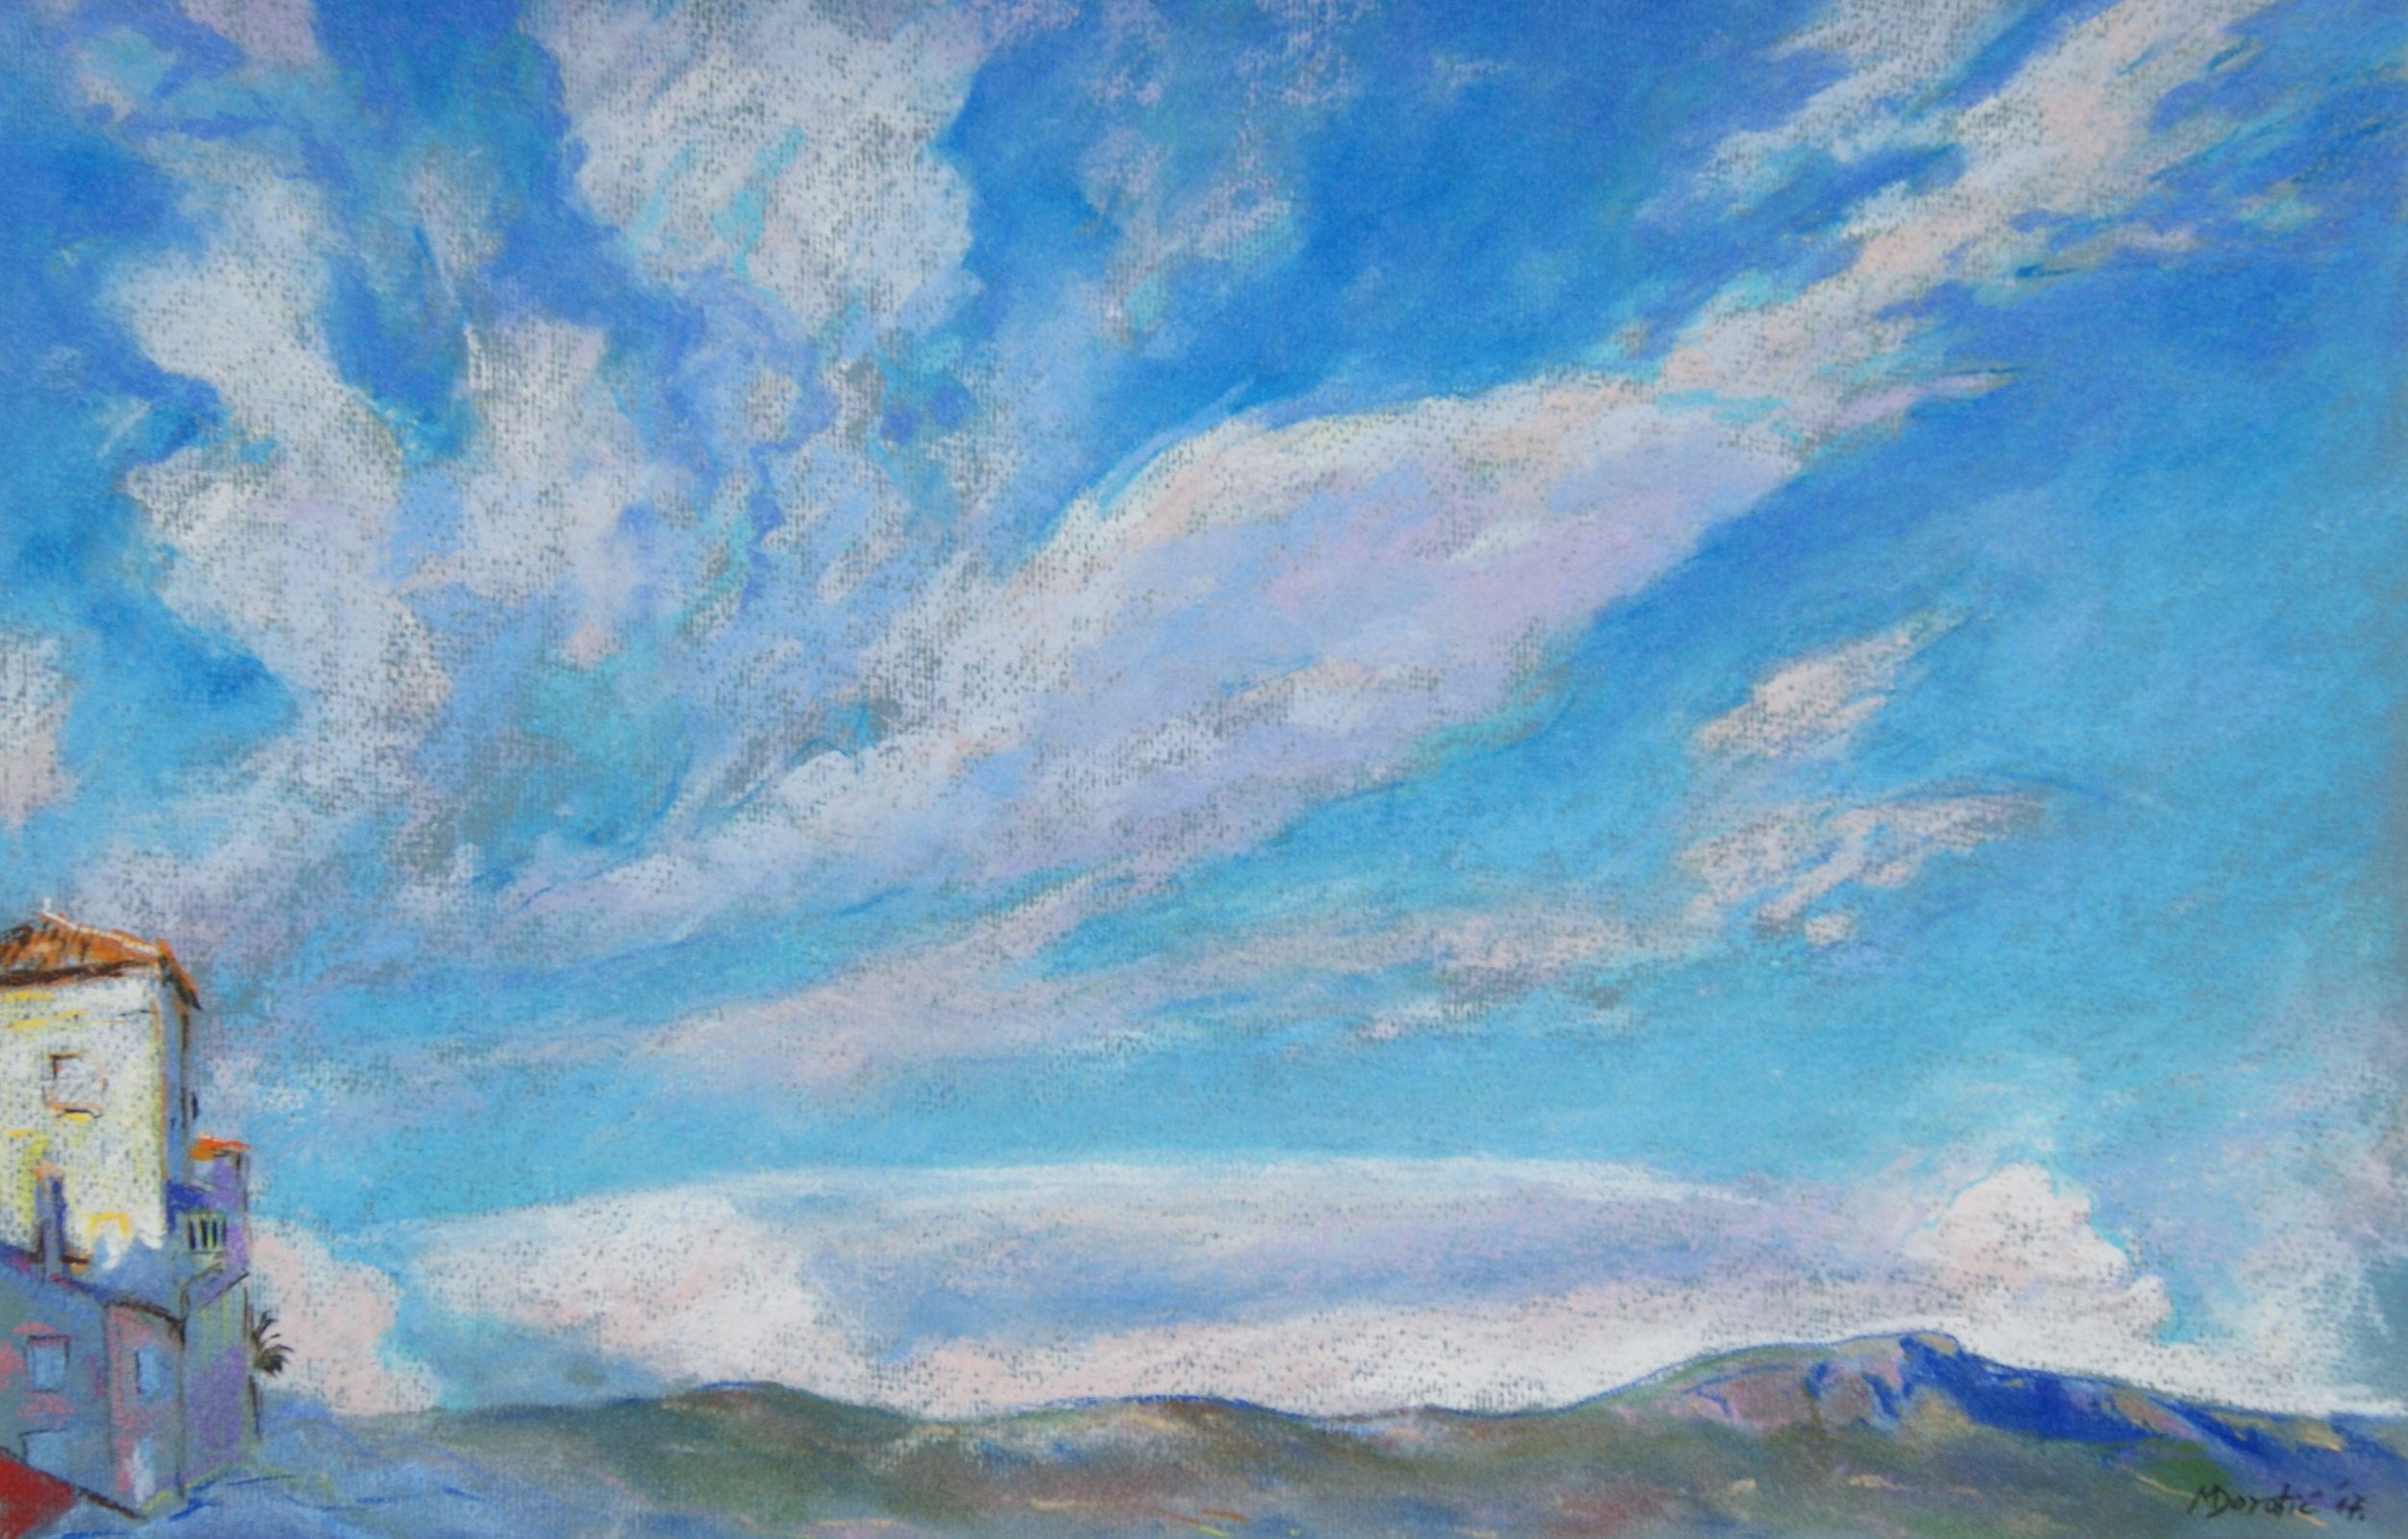
\includepdf[pages={1},noautoscale,  %
    picturecommand={\setlength\unitlength{1cm}%
         \put(2,4){\includegraphics[width=\linewidth,scale=1]{images/mihovil/d4_jaimojdom}}}]%
         {lilypond/hr/src/04_ja_i_moj_dom.pdf}
         
% \newpage
% \thispagestyle{empty}%
% \vspace*{10.5cm}
% \begin{center}
% Ova je stranica namjerno ostavljena prazna.\\
% Diese Seite wurde mit Absicht leer gelassen.
% \end{center}

\vfill

%pjesma 5
%Pokušaj uvrštavanja slike u sliku
\newpage
\phantomsection
\begin{minipage}[b]{0.5\linewidth}
\addcontentsline{toc}{section}{\texorpdfstring{{\rednifont\doccolor5.}\hspace{\onedigitspacing}}{}NIŠTA NE MOŽE NAS ODVOJITI \ttfamily(Rim 8,35.37-39)}
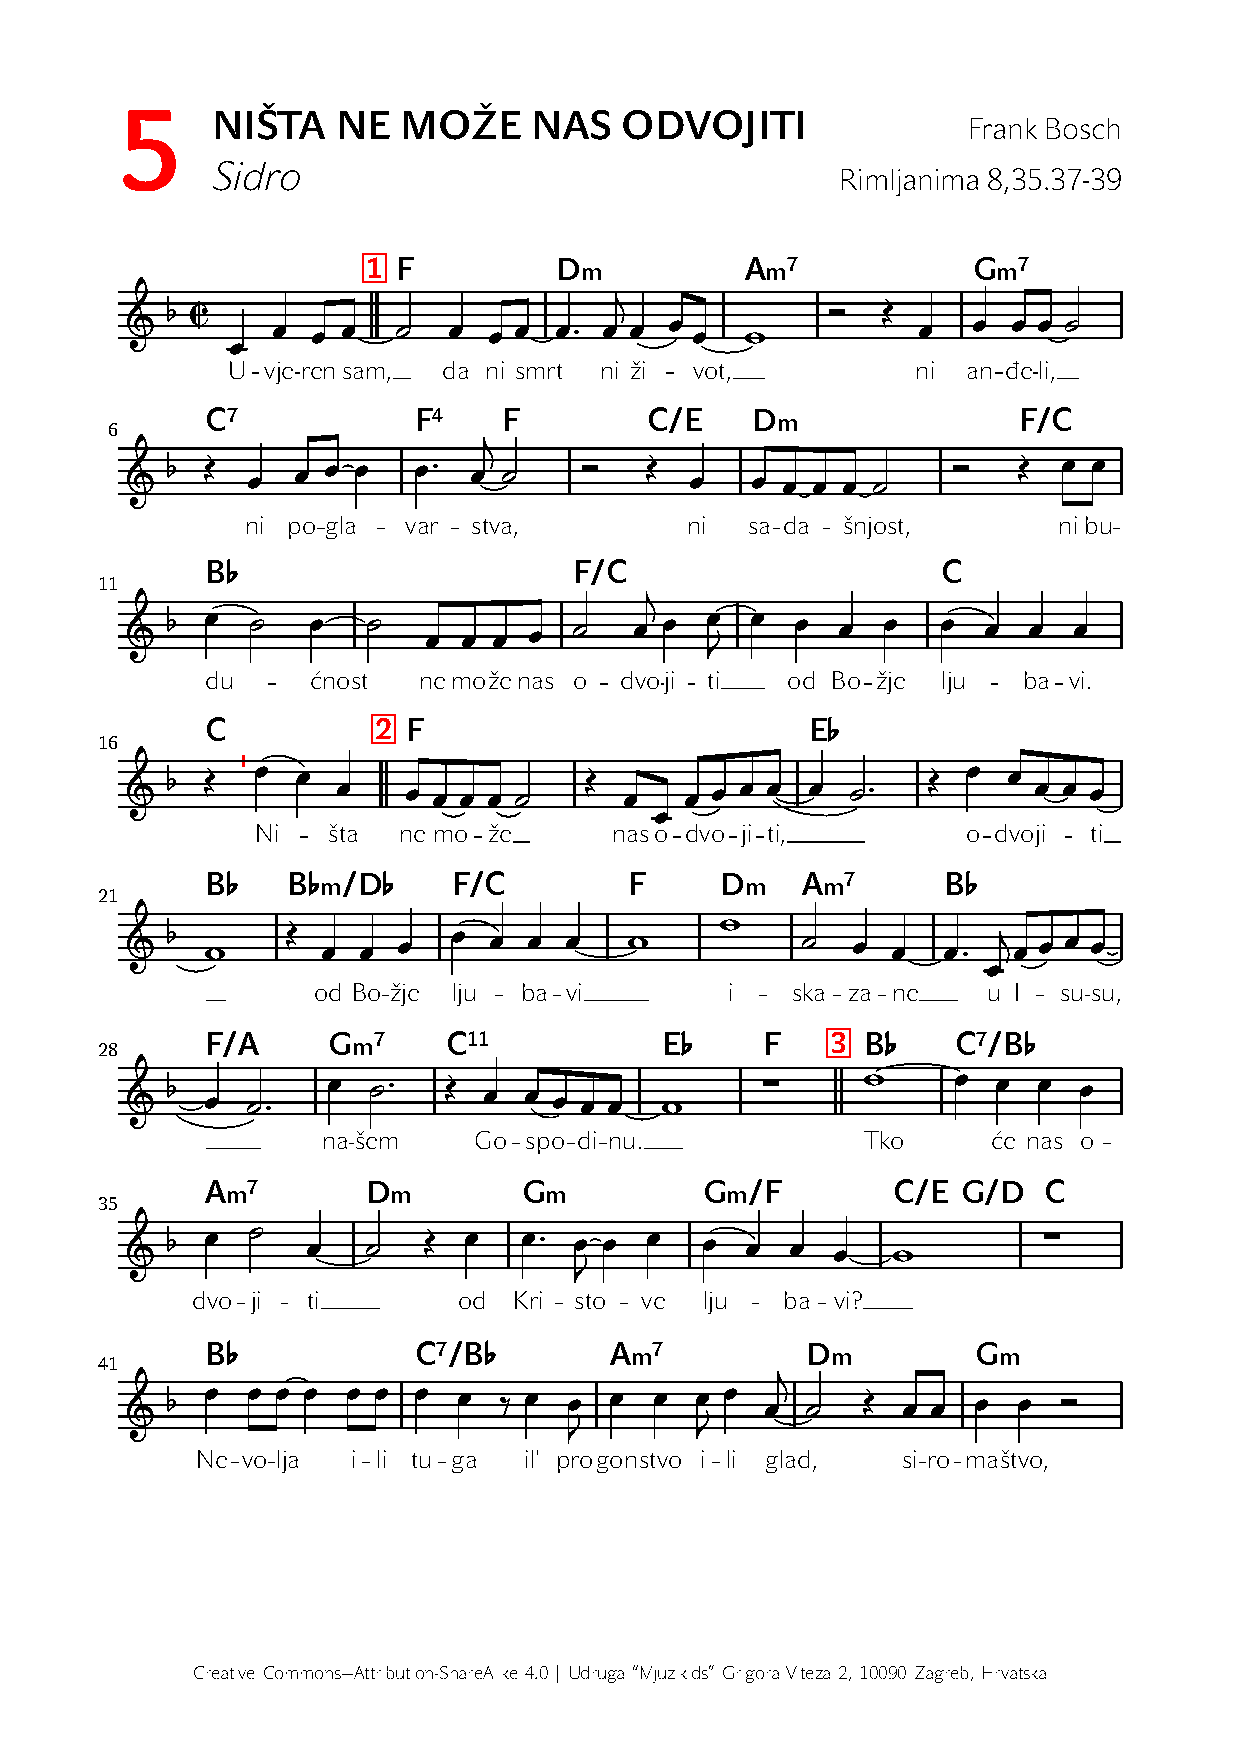
\includepdf[pages={1},noautoscale]{lilypond/hr/src/05_nista_ne_moze_nas_odvojiti.pdf}
\end{minipage}

\newpage

\includepdf[pages={2},noautoscale, %
    picturecommand={\setlength\unitlength{1cm}%
         \put(2,5){\includegraphics[width=\linewidth,scale=1]{images/mihovil/e5_nistanemoze}}}]%
         {lilypond/hr/src/05_nista_ne_moze_nas_odvojiti.pdf}

%pjesma 6
\newpage
\phantomsection
\begin{minipage}[b]{0.5\linewidth}
\addcontentsline{toc}{section}{\texorpdfstring{{\rednifont\doccolor6.}\hspace{\onedigitspacing}}{}TVOJA RIJEČ \ttfamily(Ps 119,9.105)}
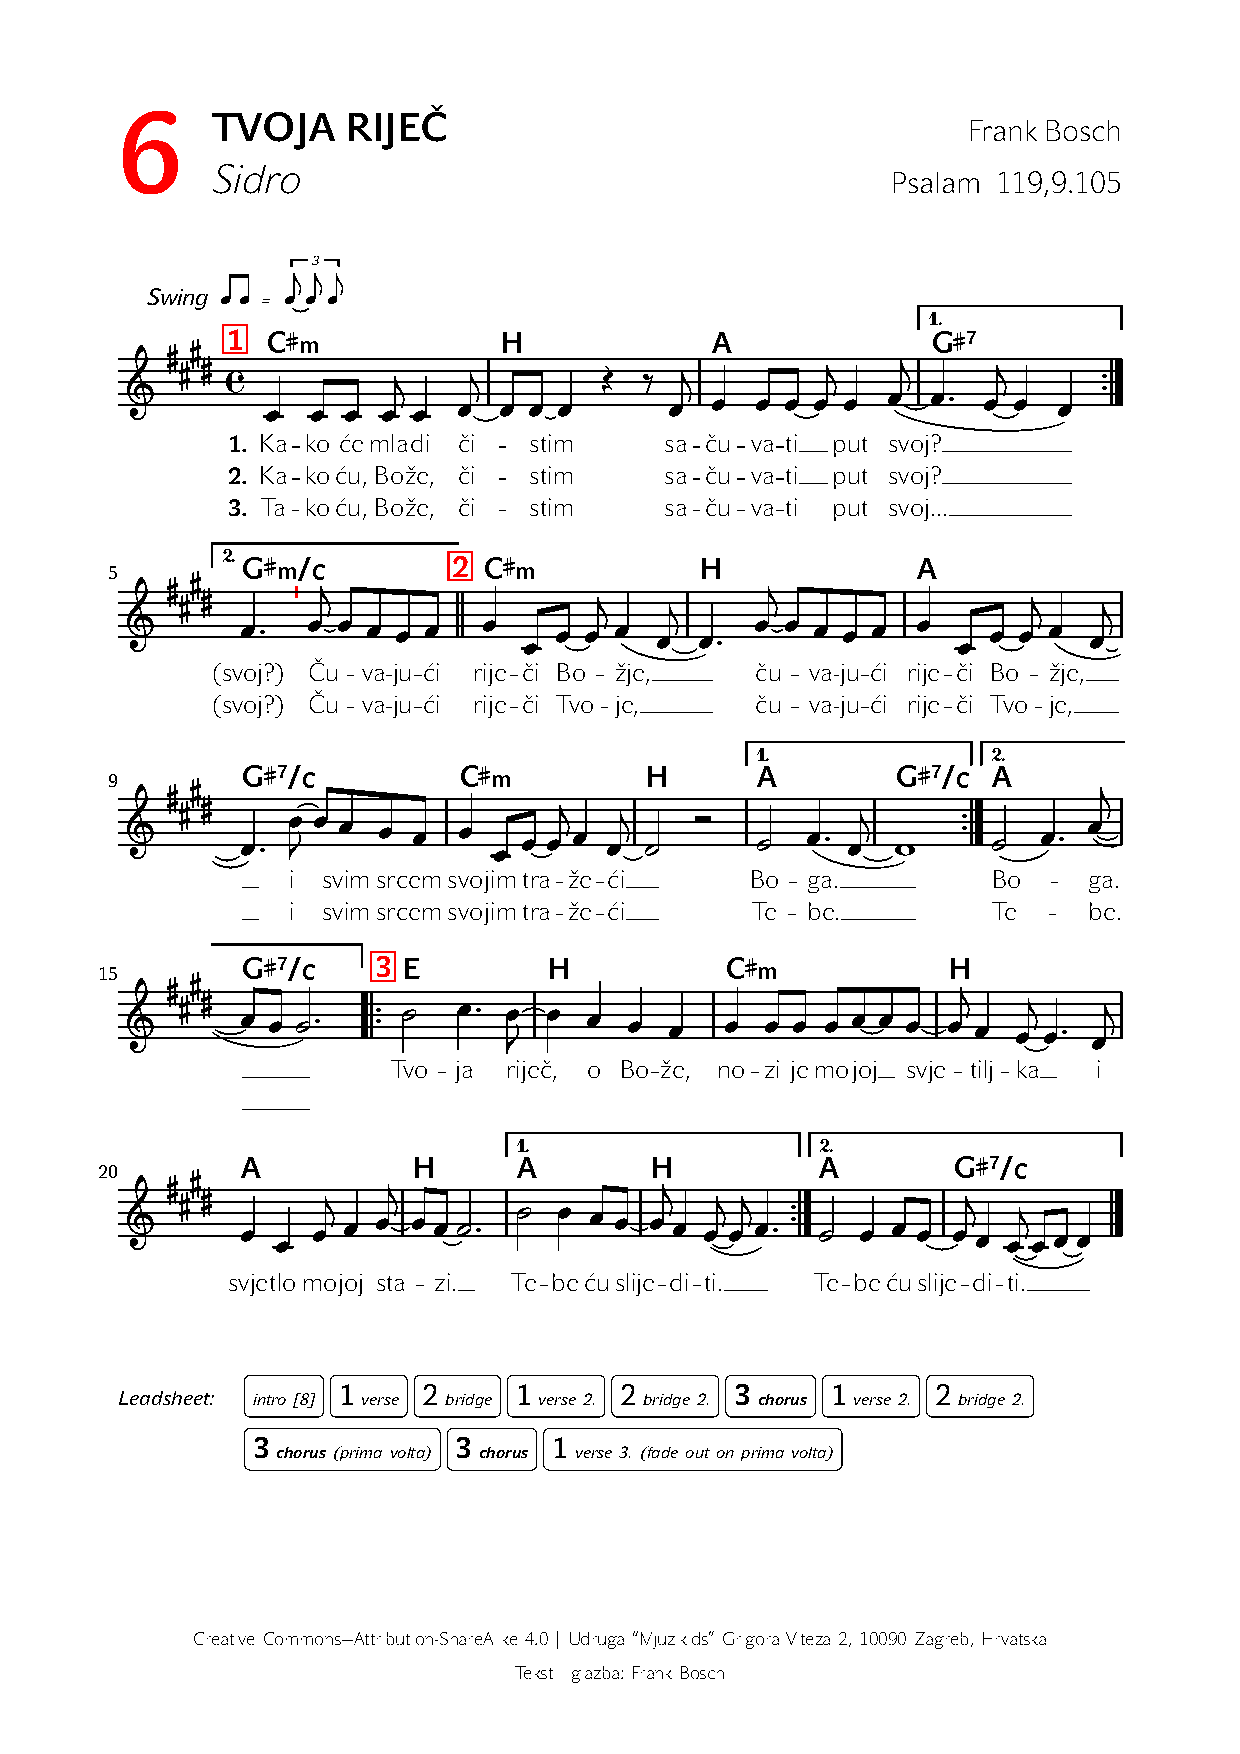
\includepdf[pages={1},noautoscale]{lilypond/hr/src/06_tvoja_rijec.pdf}
\end{minipage}

\newpage
\begin{center}
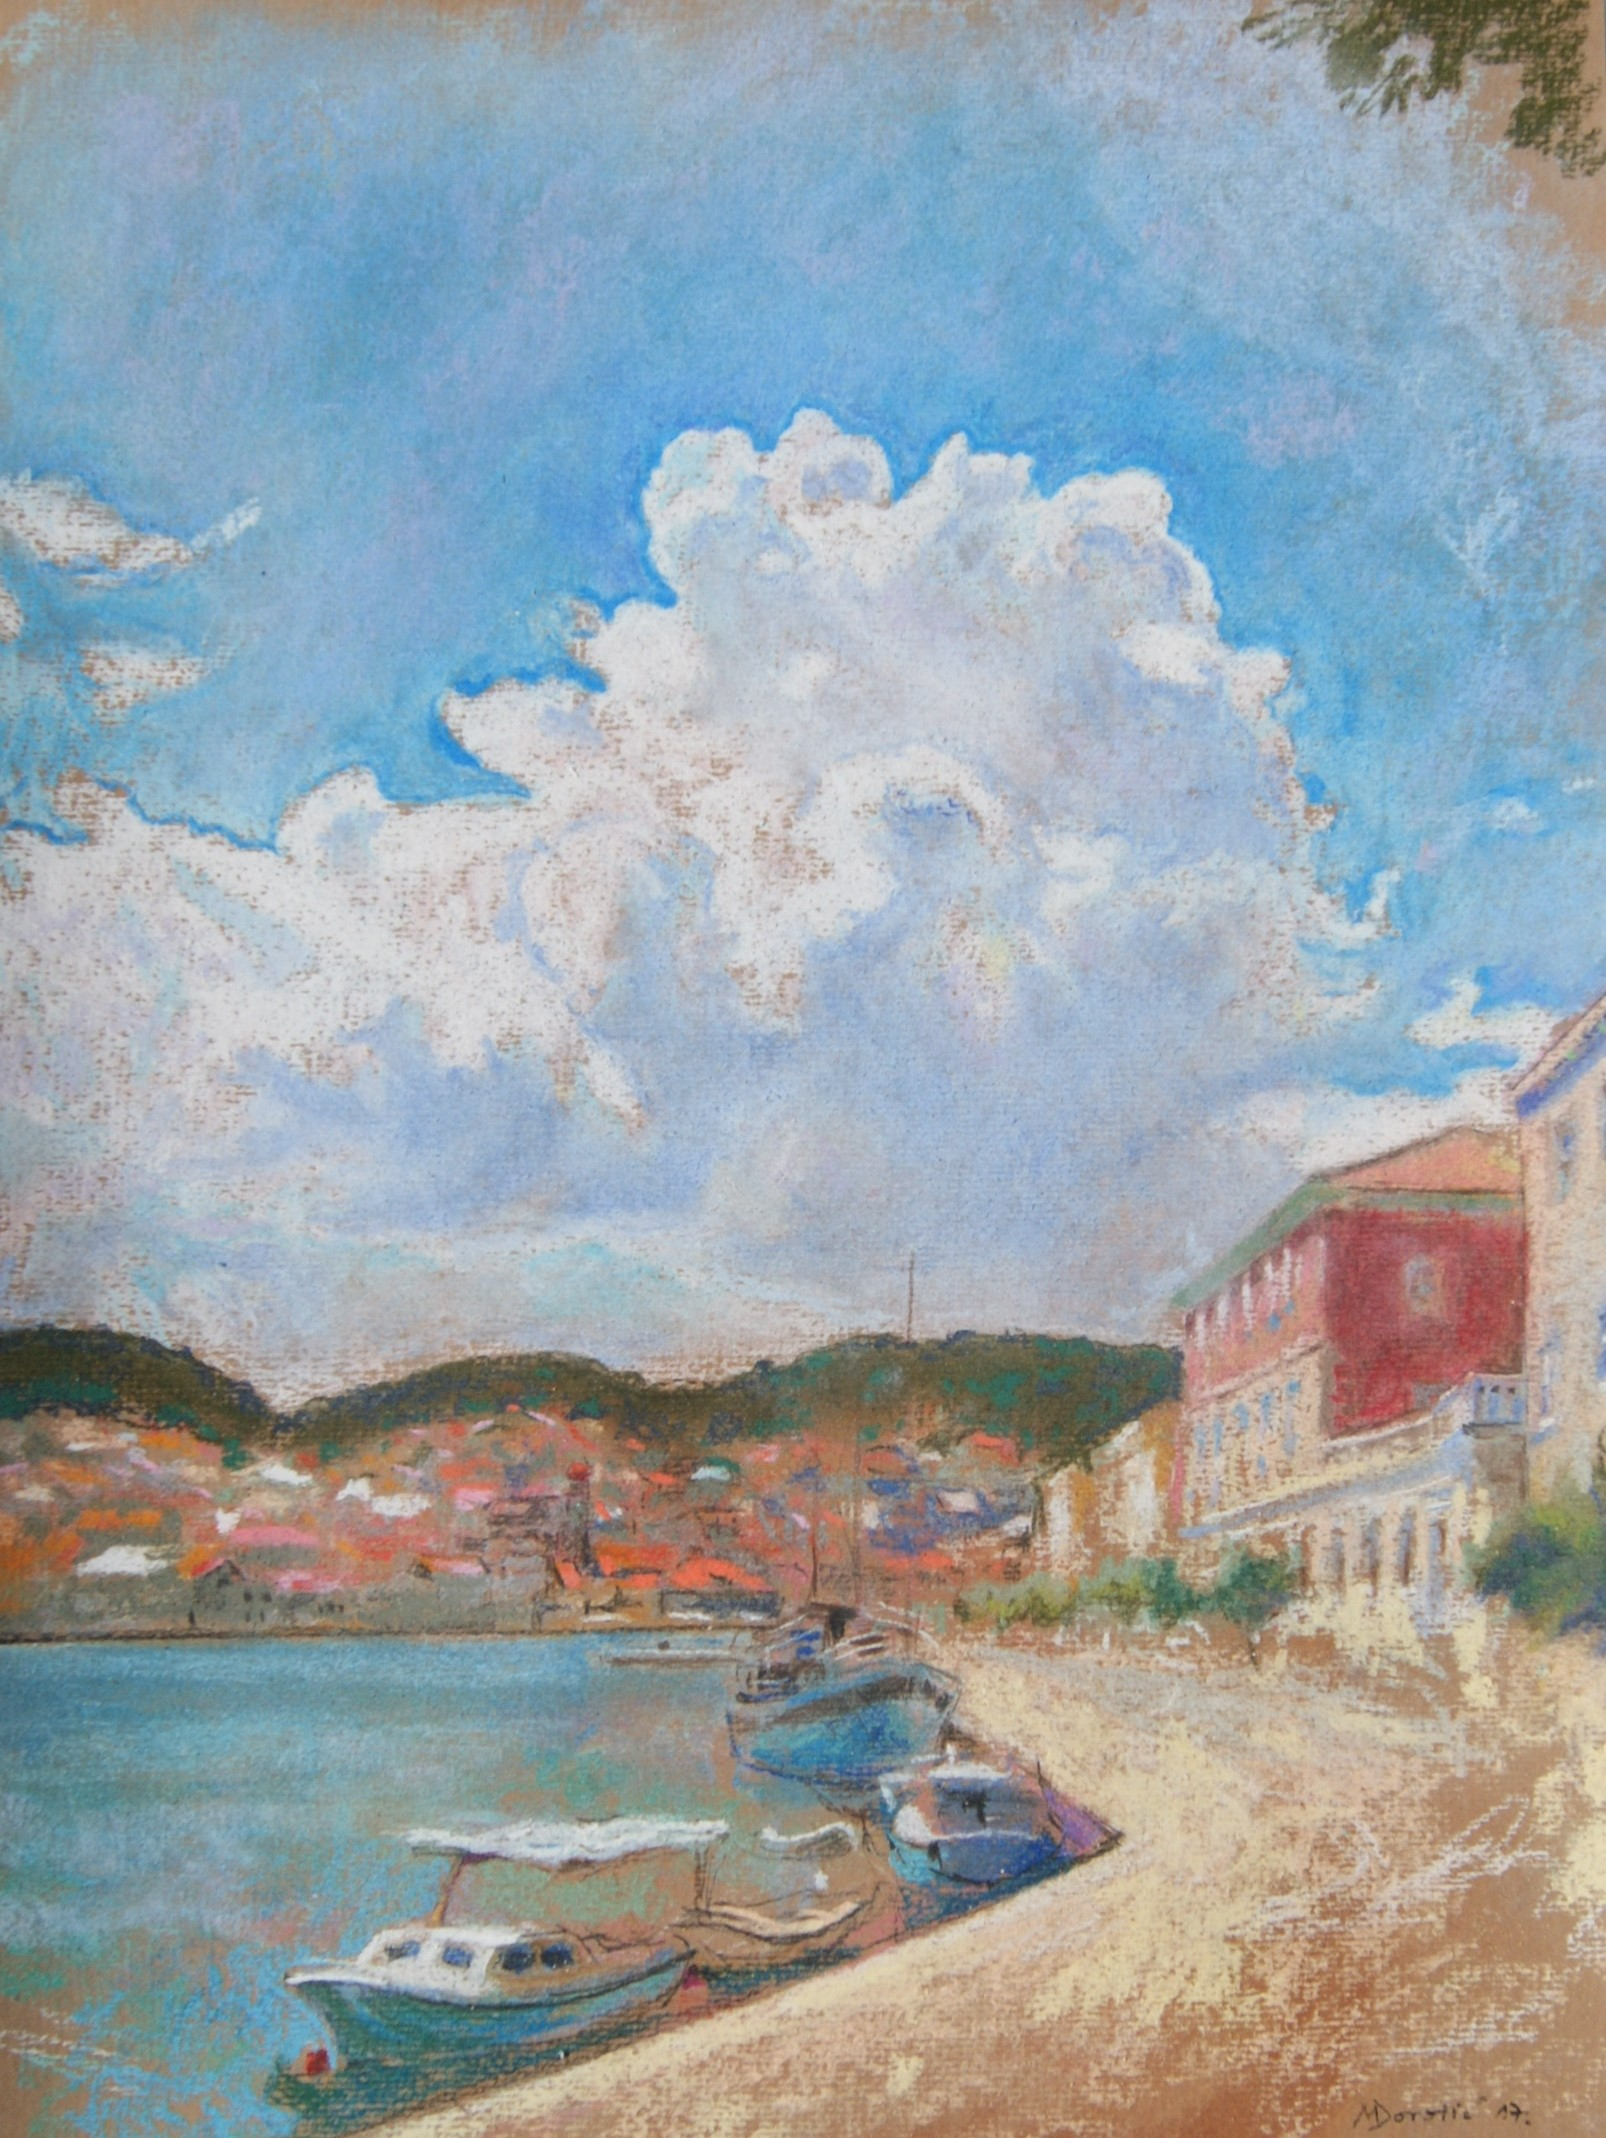
\includegraphics[width=\linewidth]{images/mihovil/pejza_13}
\end{center}

%pjesma 7
\newpage
\phantomsection
\begin{minipage}[b]{0.5\linewidth}
\addcontentsline{toc}{section}{\texorpdfstring{{\rednifont\doccolor7.}\hspace{\onedigitspacing}}{}BLAGOSLIVLJAJ BOGA \ttfamily(Ps 103,1-5)}
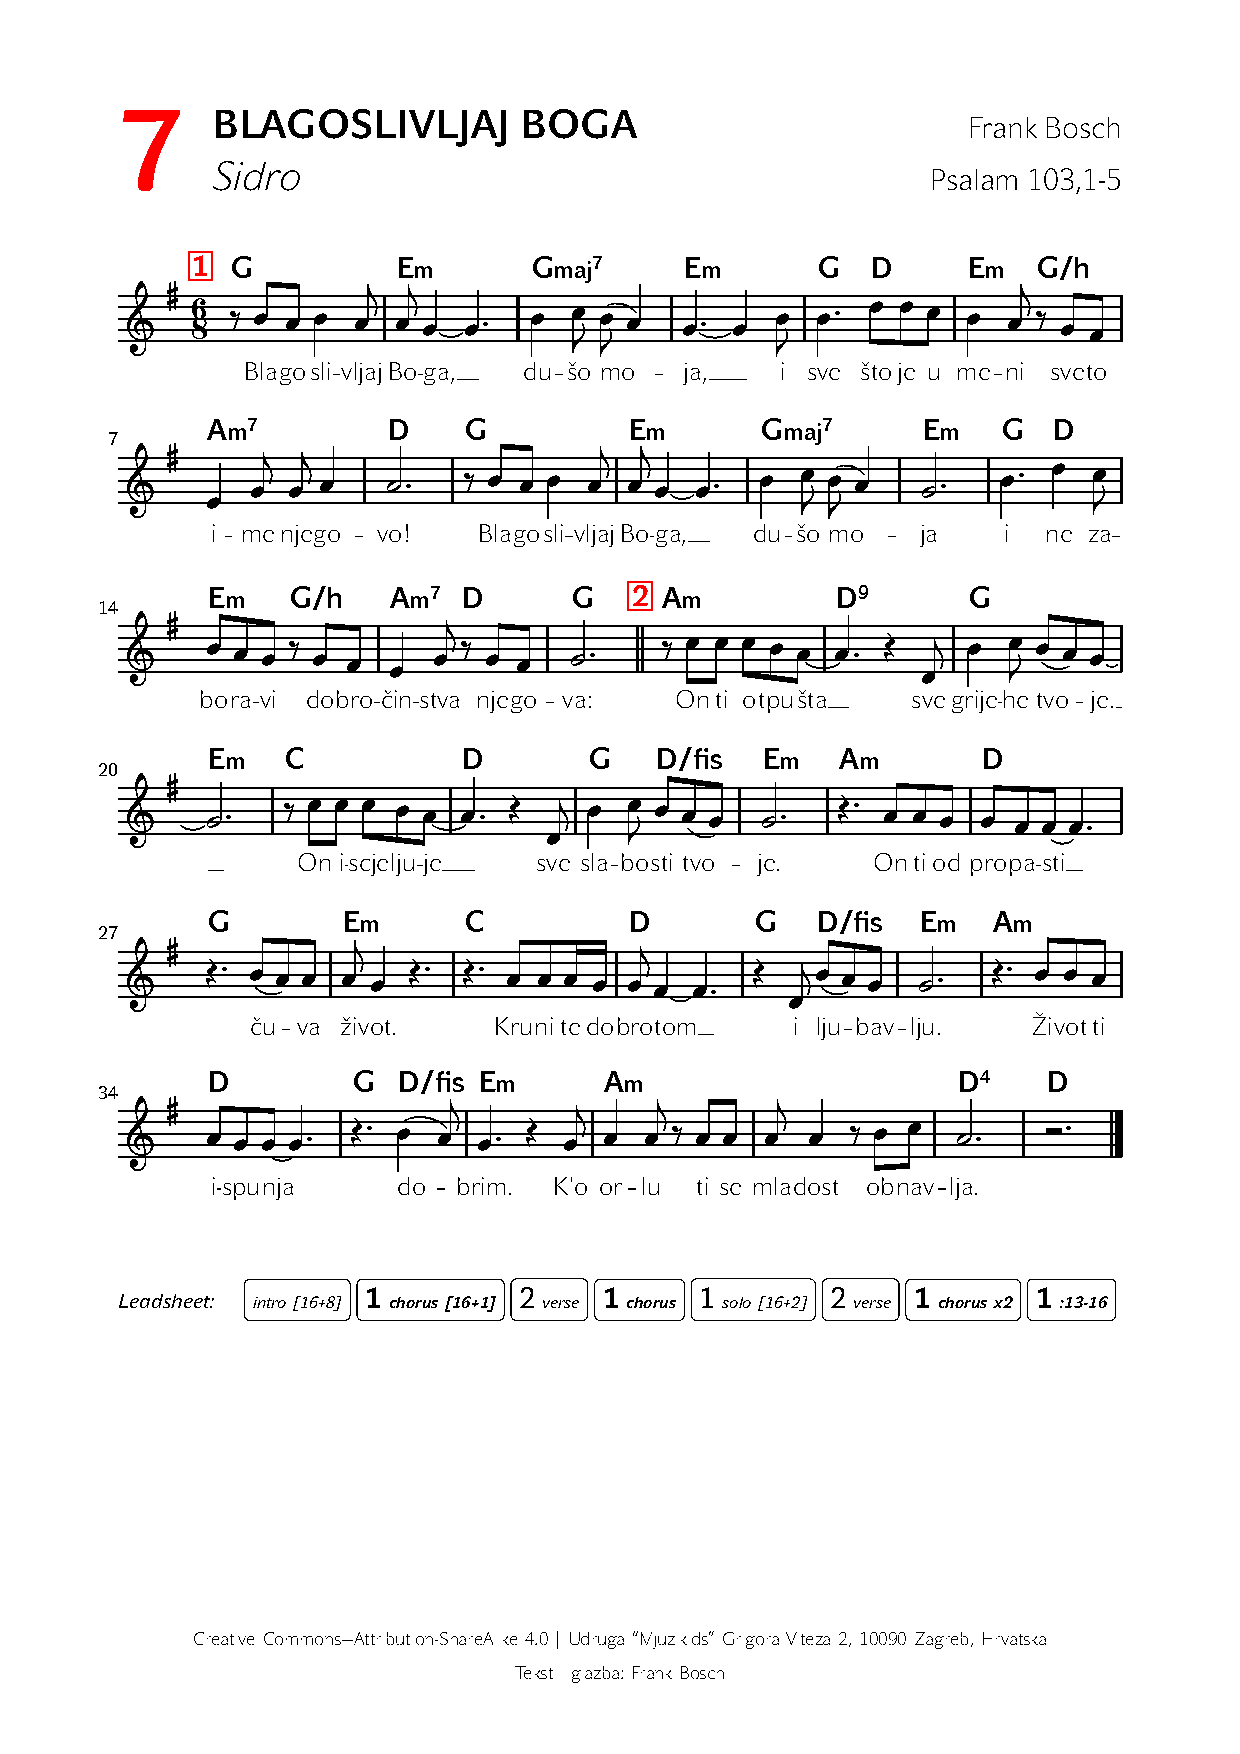
\includepdf[pages={1},noautoscale]{lilypond/hr/src/07_blagoslivljaj_boga.pdf}
\end{minipage}

\newpage
\begin{center}
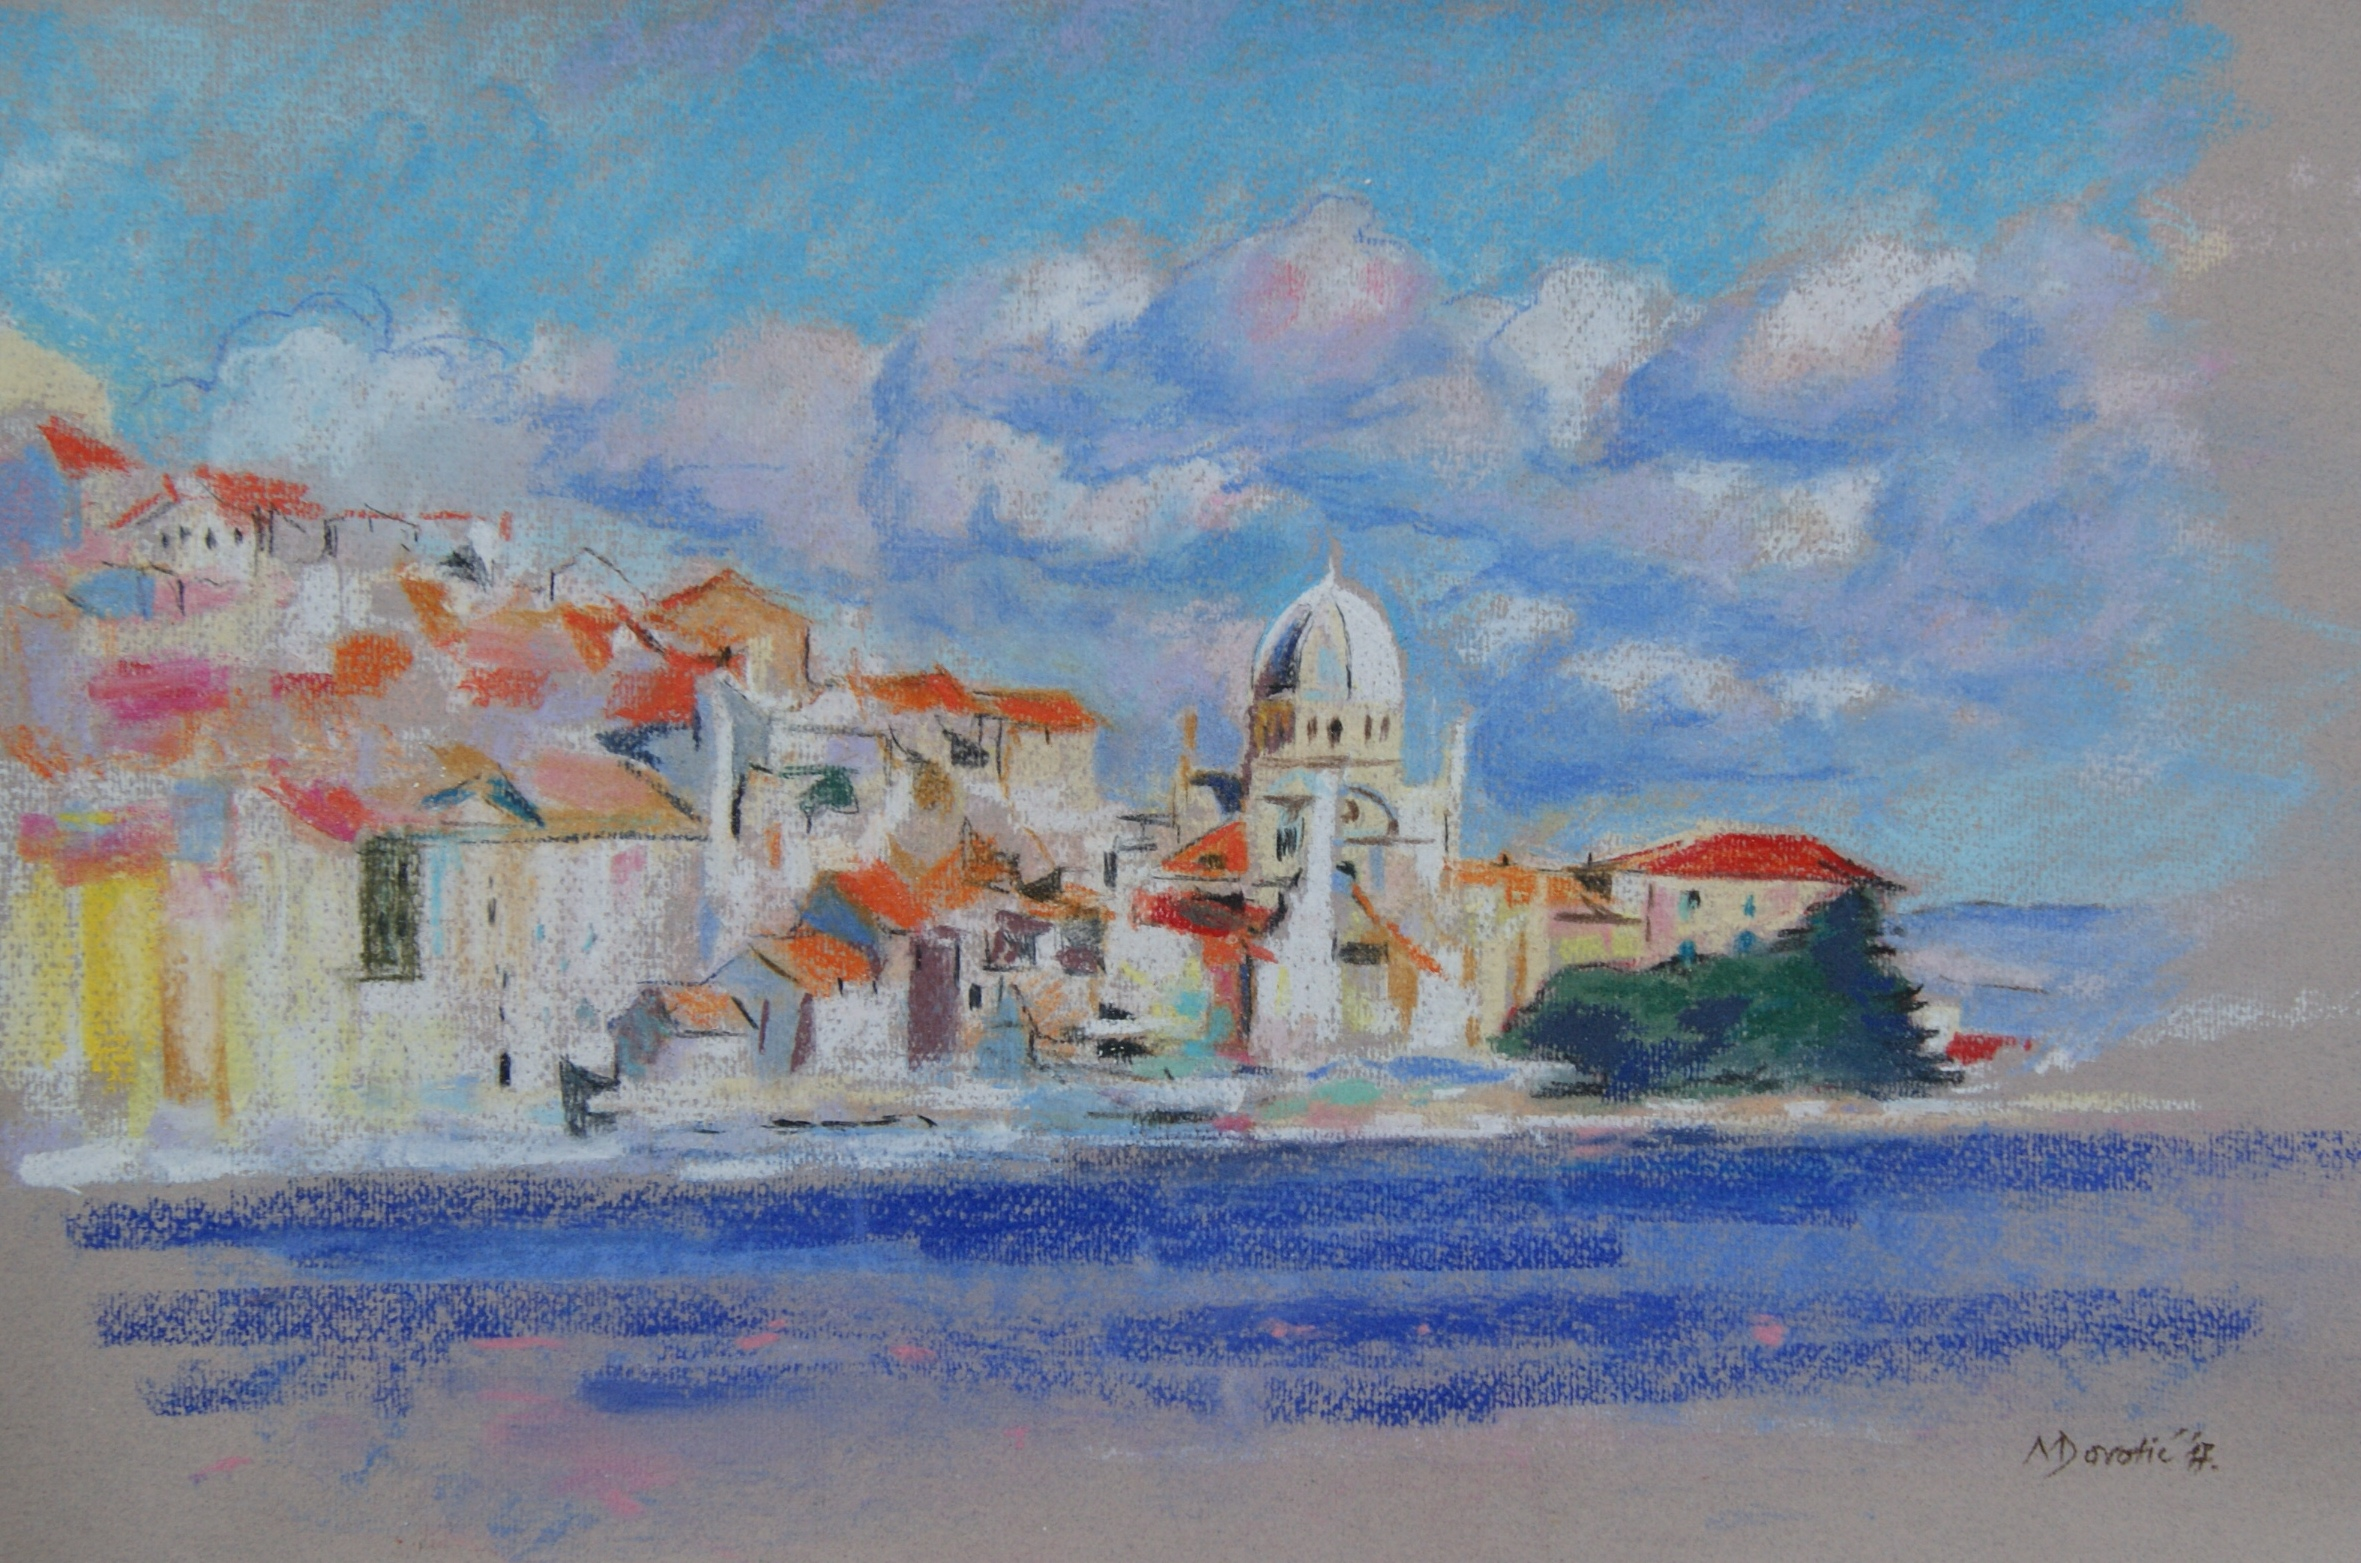
\includegraphics[width=\linewidth]{images/mihovil/g7_blagoslivljajboga}\\
\vspace*{1cm}
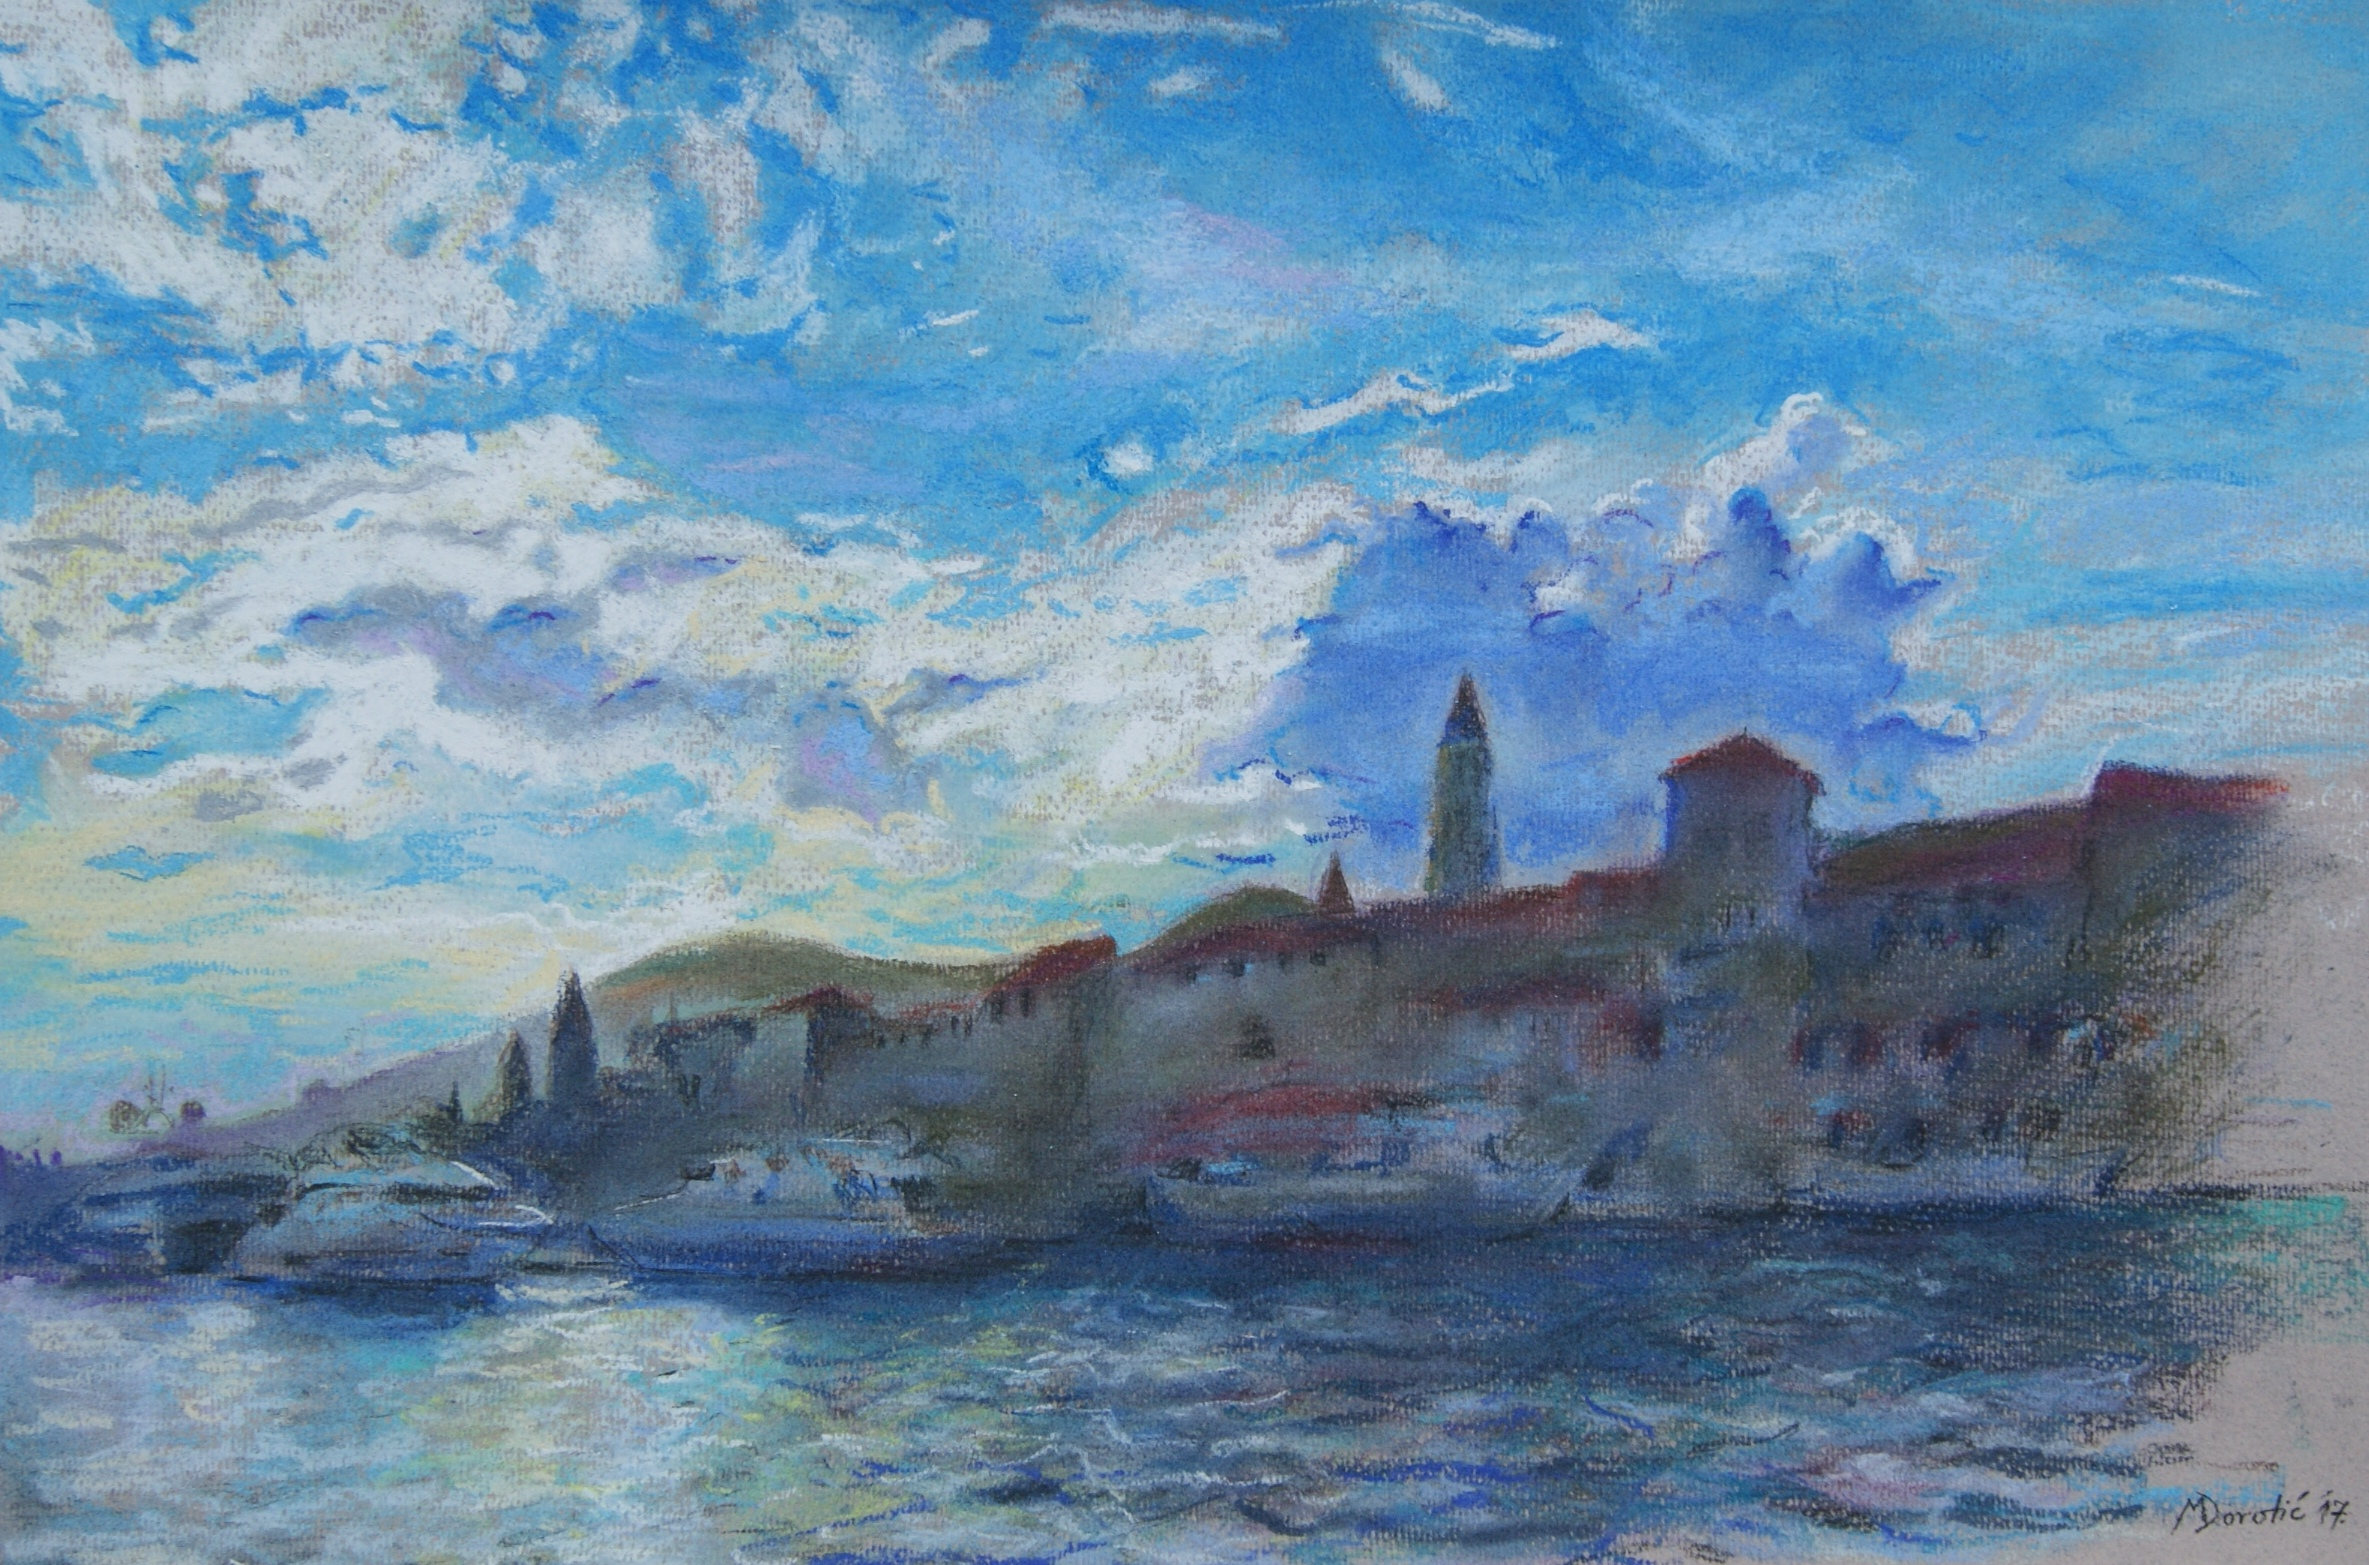
\includegraphics[width=\linewidth]{images/mihovil/f6_tvojarijec}
\end{center}

%pjesma 8
\newpage
\phantomsection
\begin{minipage}[b]{0.5\linewidth}
\addcontentsline{toc}{section}{\texorpdfstring{{\rednifont\doccolor8.}\hspace{\onedigitspacing}}{}KLIČI BOGU ZEMLJO SVA \ttfamily(Ps 100)}
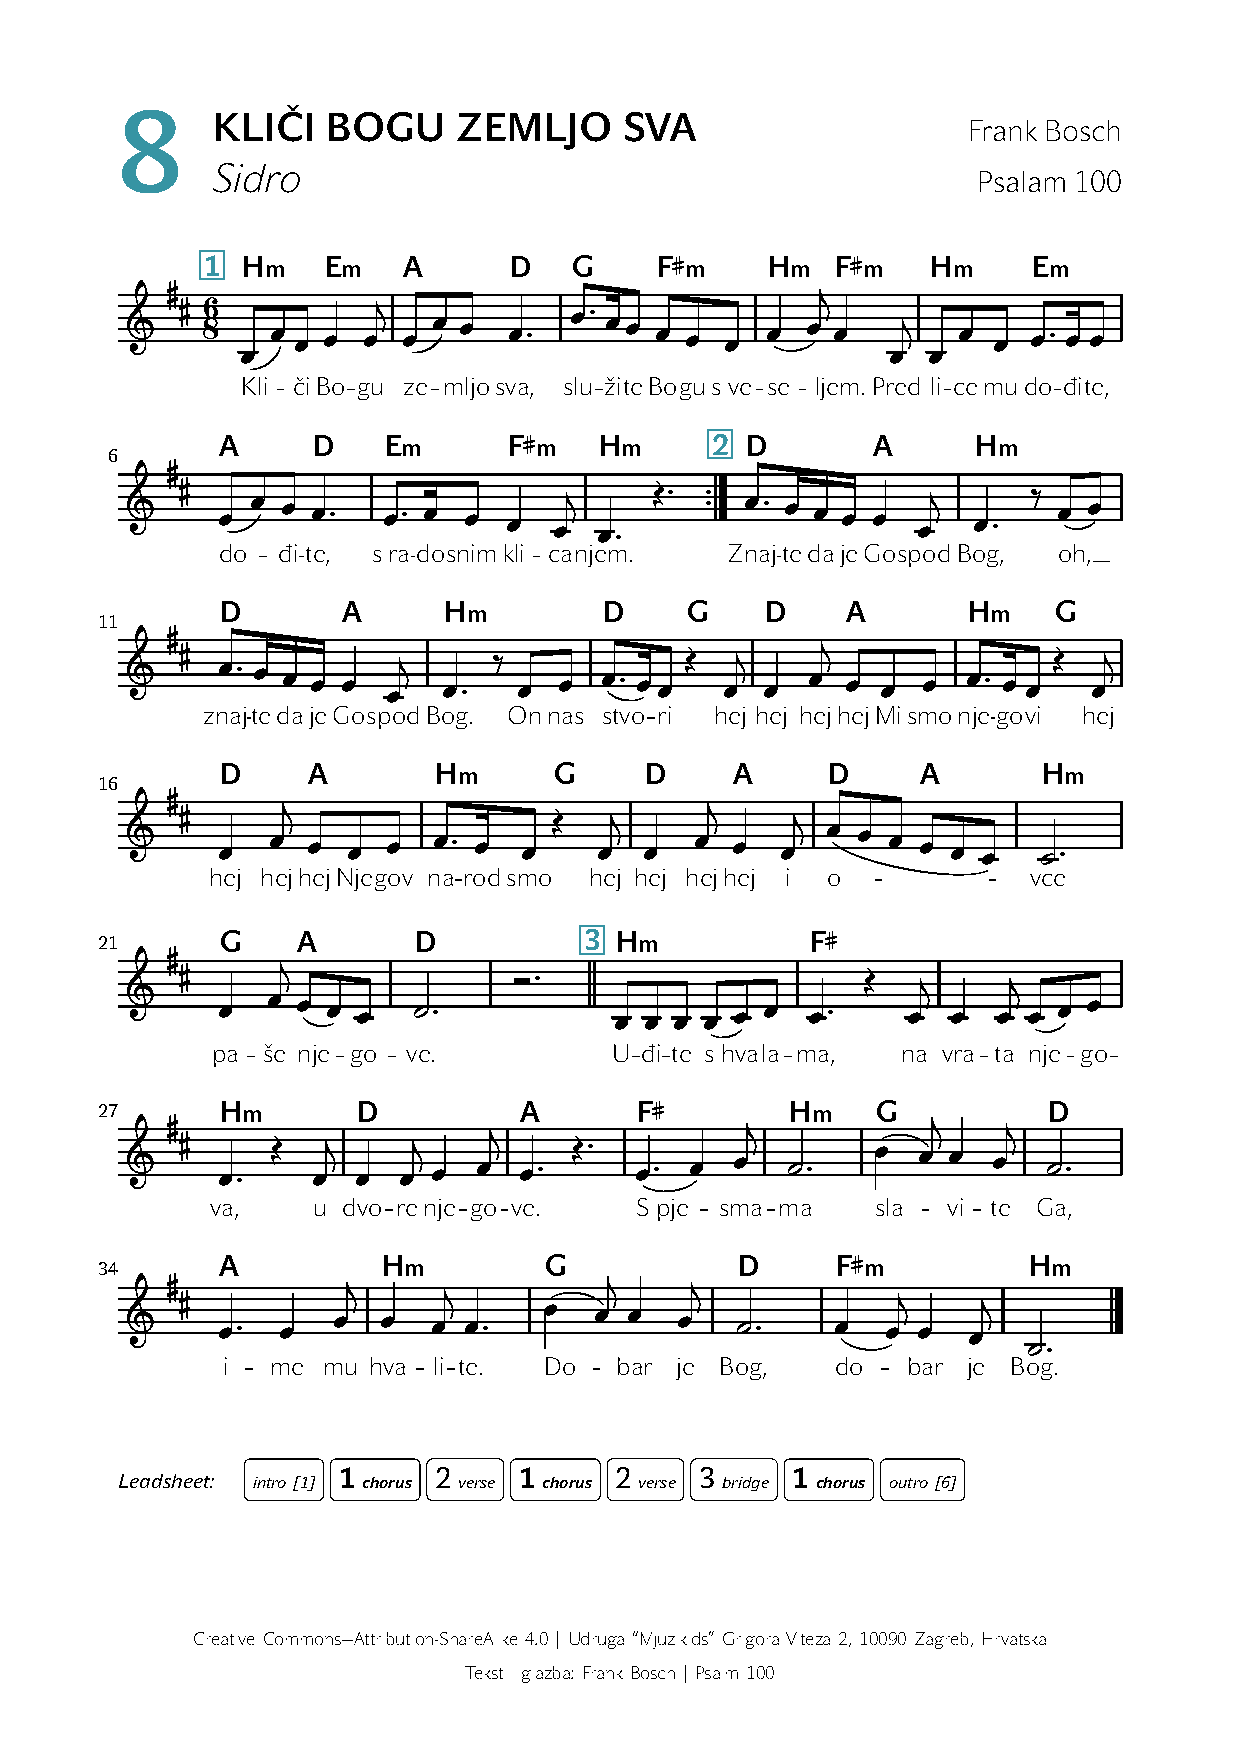
\includepdf[pages={1},noautoscale]{lilypond/hr/src/08_klici_bogu_zemljo_sva.pdf}
\end{minipage}

\newpage
\begin{center}
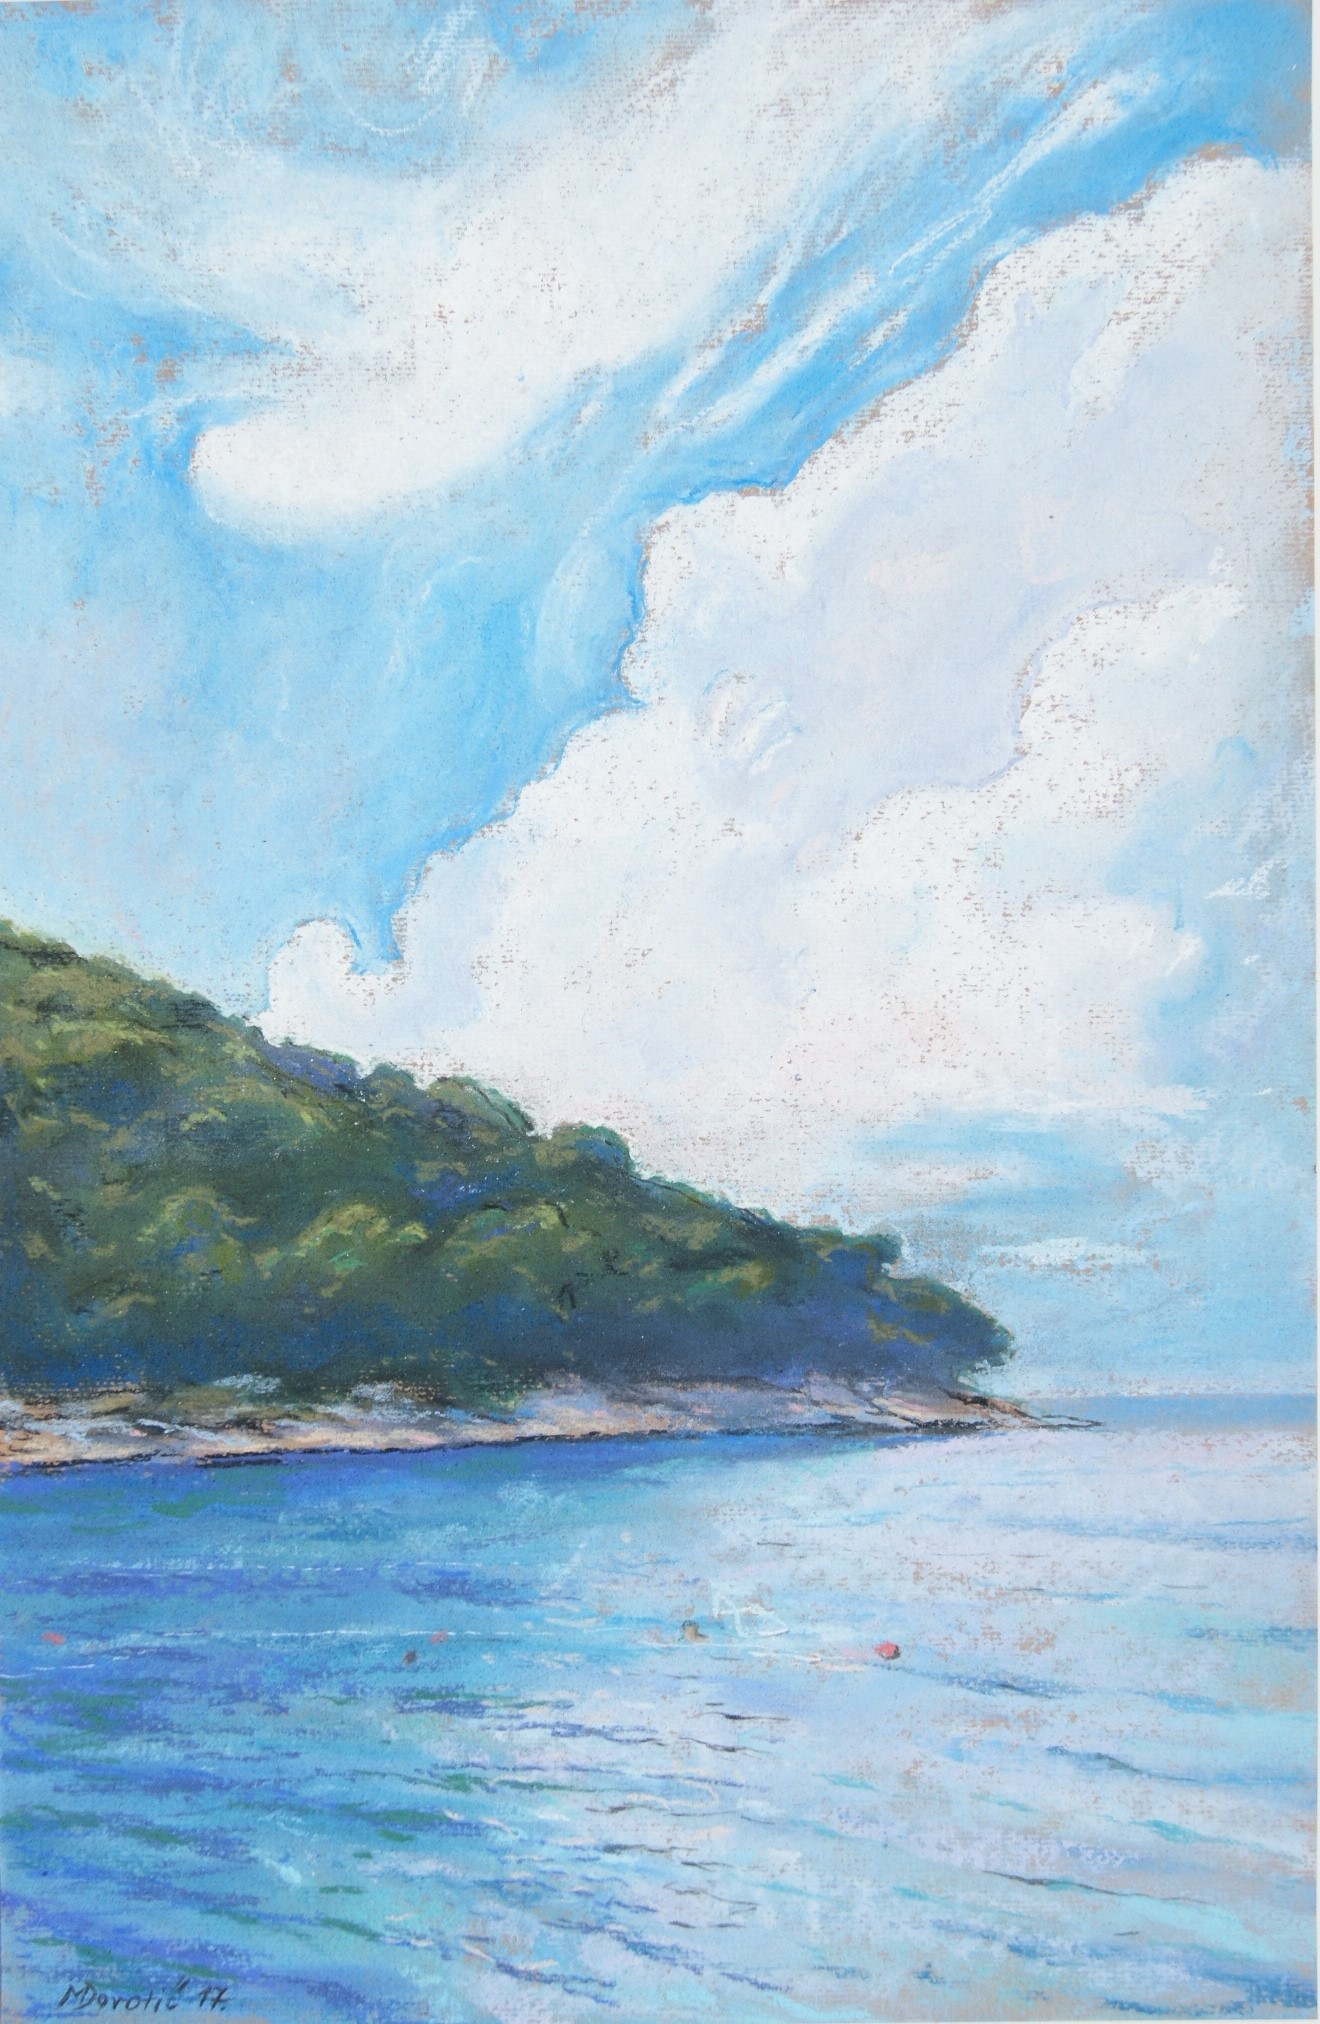
\includegraphics[width=0.9\linewidth]{images/mihovil/h8_klicibogu}
\end{center}

%pjesma 9
\newpage
\phantomsection
\begin{minipage}[b]{0.5\linewidth}
\addcontentsline{toc}{section}{\texorpdfstring{{\rednifont\doccolor9.}\hspace{\onedigitspacing}}{}PUSTINJOM LUTAMO MI}
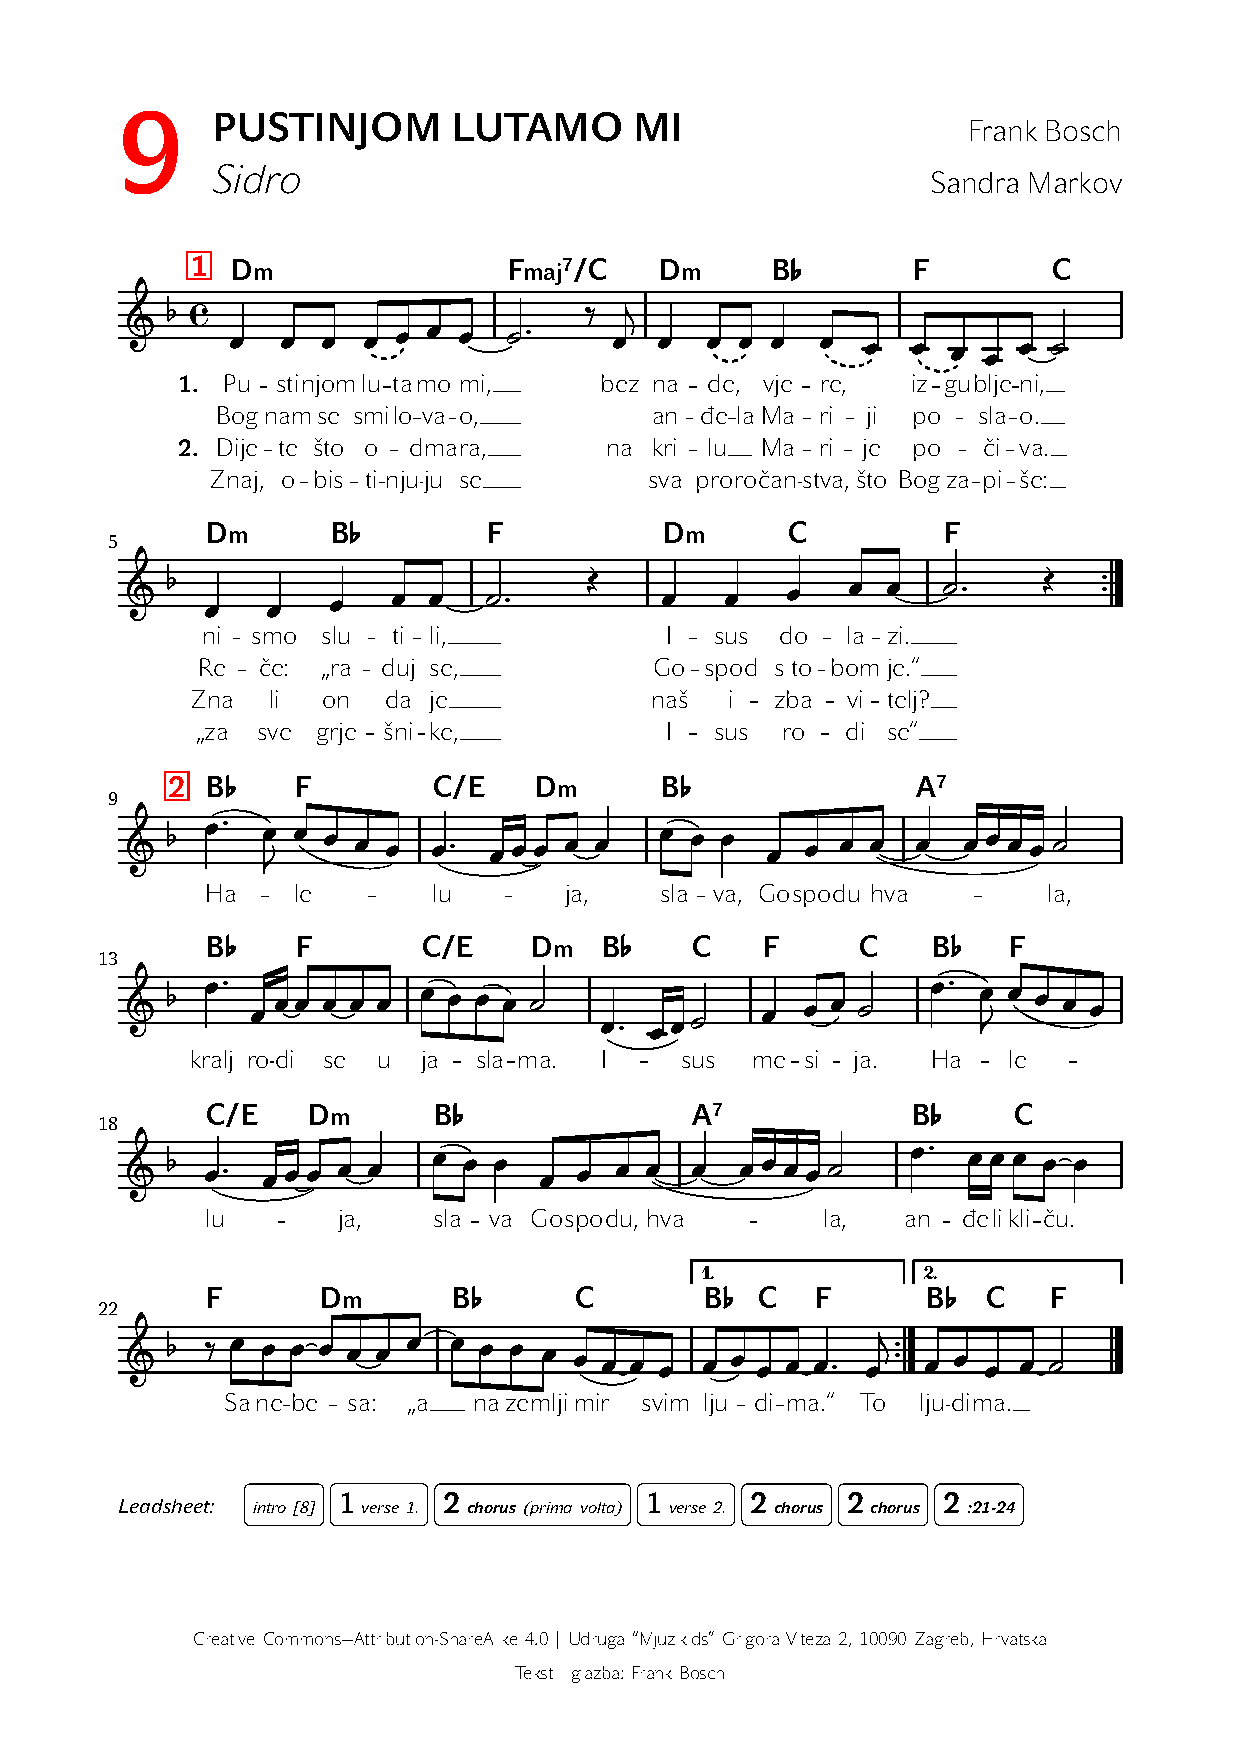
\includepdf[pages={1},noautoscale]{lilypond/hr/src/09_pustinjom_lutamo_mi.pdf}
\end{minipage}

\newpage
\begin{center}
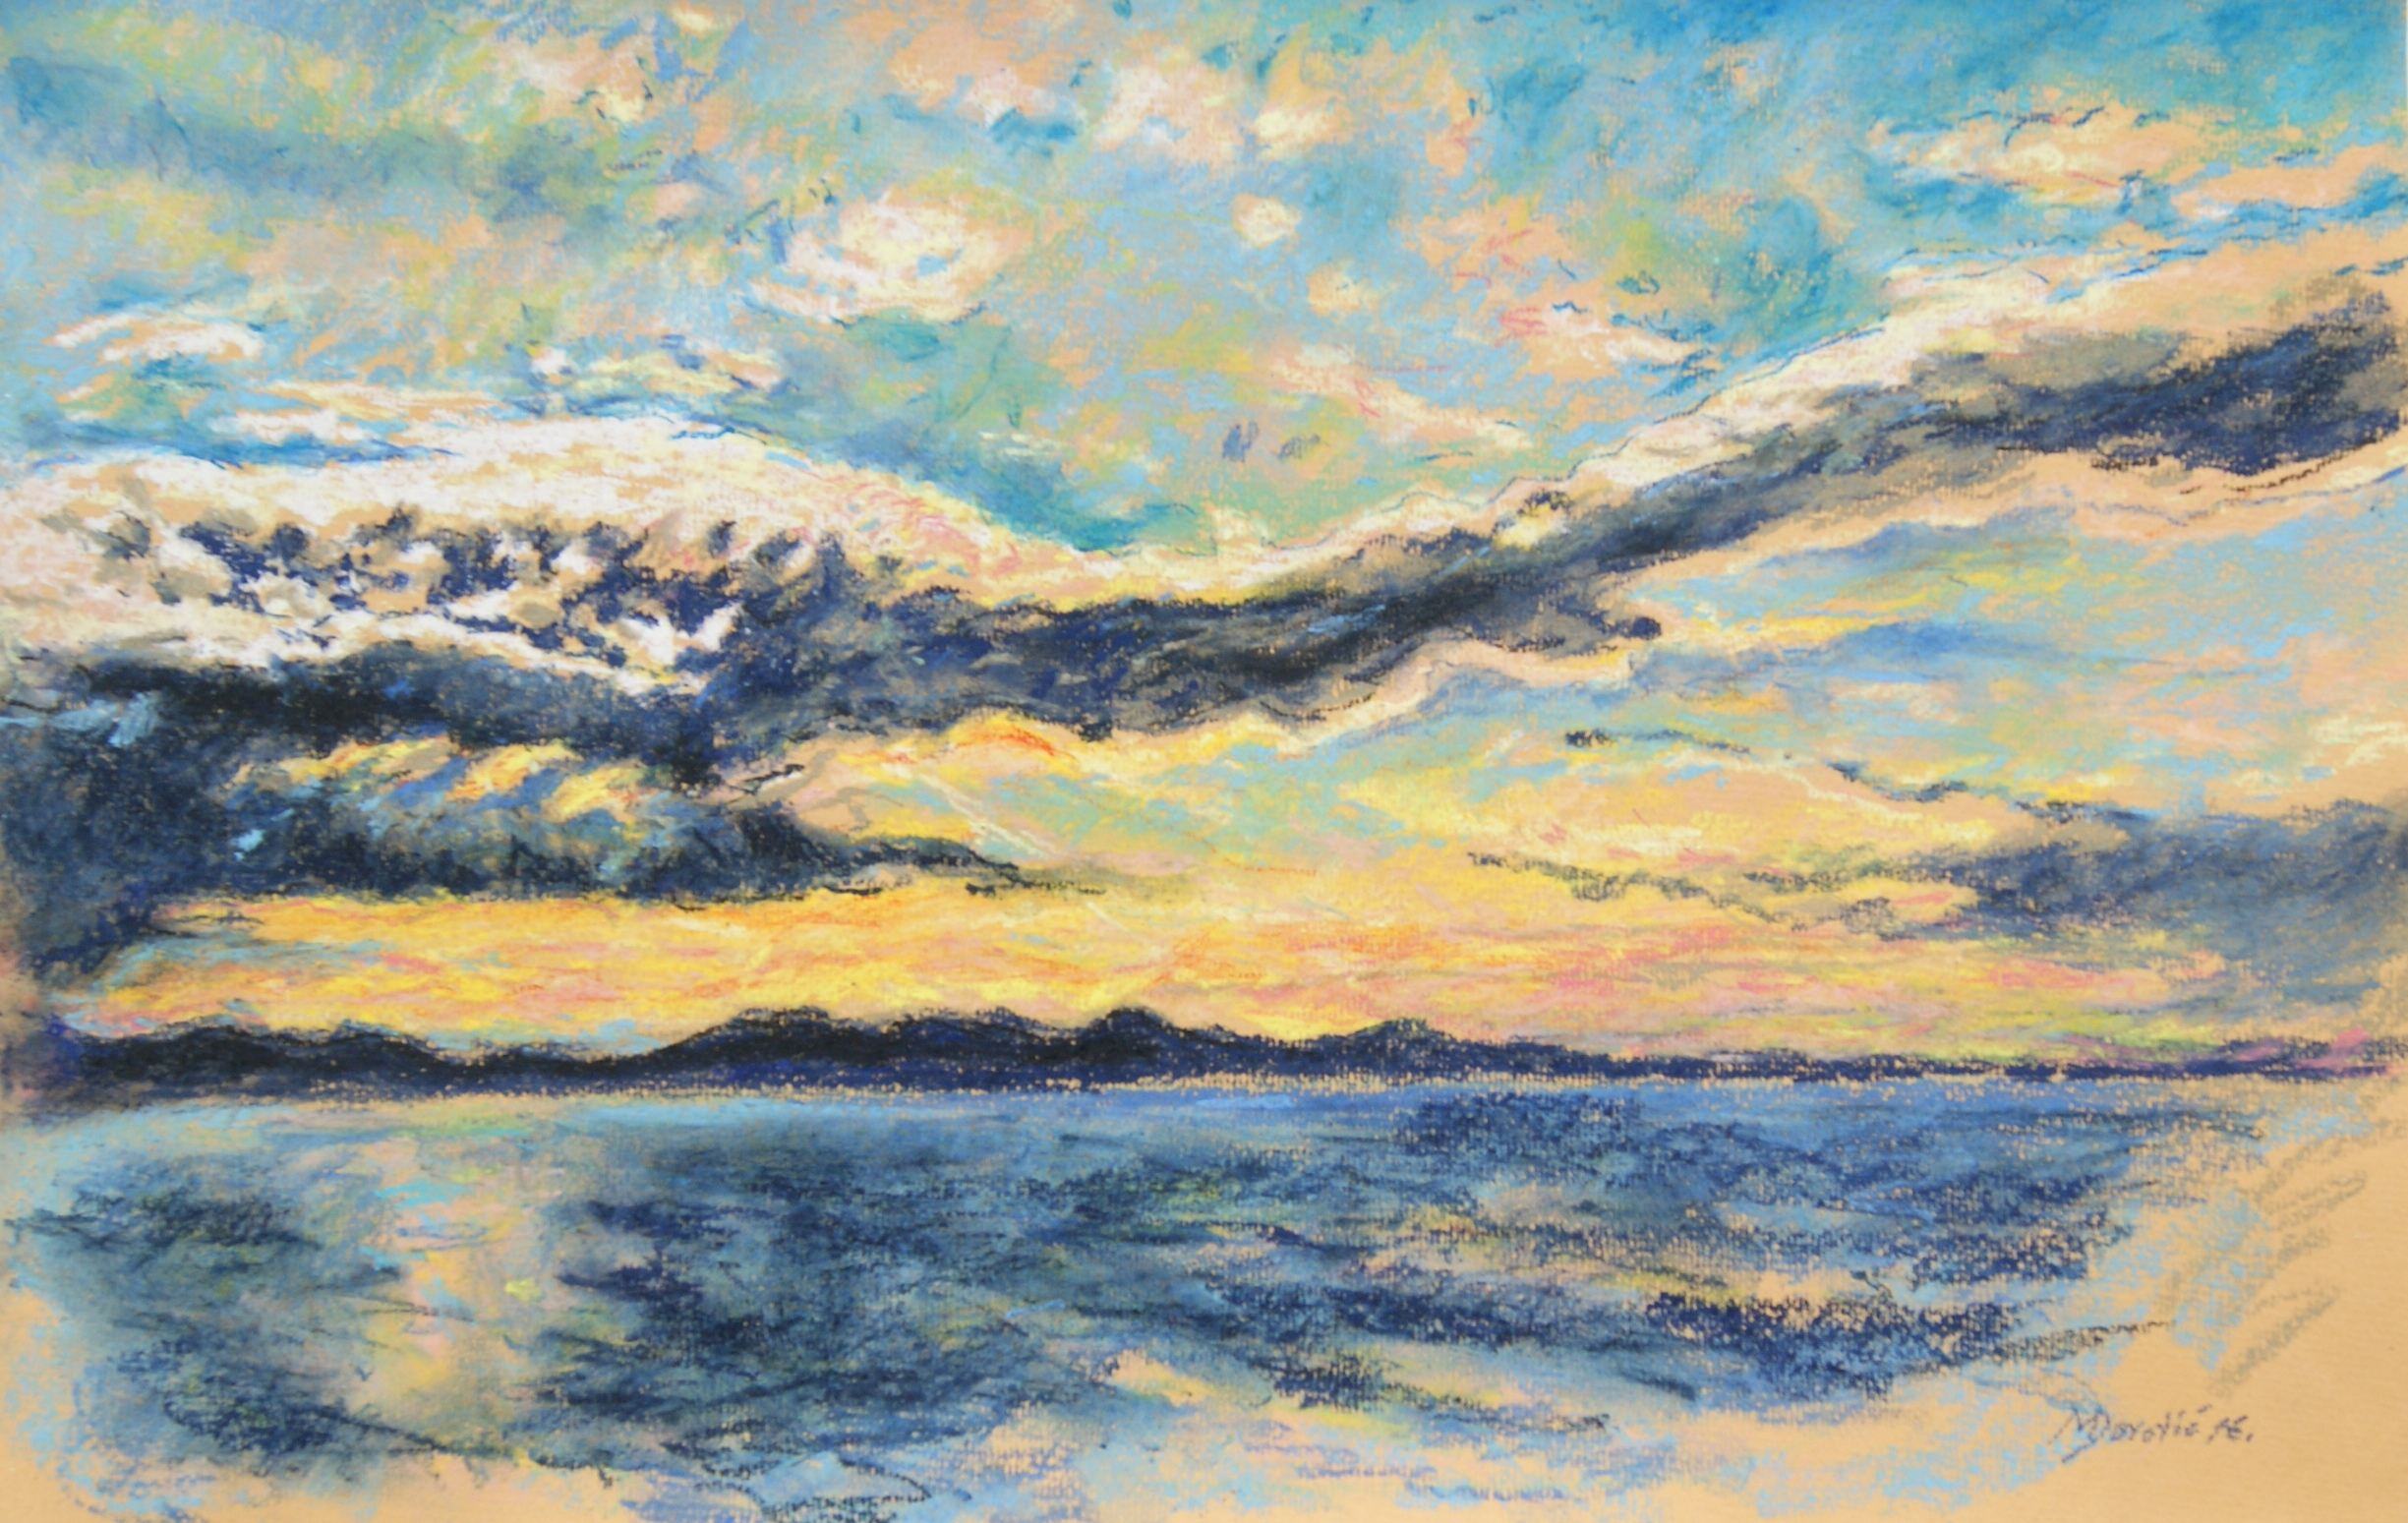
\includegraphics[width=\linewidth]{images/mihovil/i9_pustinjomlutamo}
\end{center}

\vspace*{1mm}
\begin{center}

	\Large{\parbox{\linewidth}{
		\begin{center}
		{\Large
		\texttt{
			\textit{"Narod koji je u tmini hodio svjetlost vidje veliku;
one što mrklu zemlju obitavahu
svjetlost jarka obasja."}
			}
		}
		\end{center}
		\begin{center}
		{\Large
			\texttt{{\textemdash Izaija 9,1}}
		}
		\end{center}
	}
}
\end{center}


%pjesme za djeca spava
\addtocontents{toc}{\cftpagenumbersoff{section}}
\addcontentsline{toc}{section}{\texorpdfstring{\ttfamily\hspace{7.7mm}}{}PJESME ZA DJECU}
\addtocontents{toc}{\cftpagenumberson{section}} % to restore the showing of page numbers

%pjesma 10
\newpage
\phantomsection
\begin{minipage}[b]{0.5\linewidth}
\addcontentsline{toc}{section}{\texorpdfstring{{\rednifont\doccolor10.}\hspace{\twodigitspacing}}{}SVJETLO JE ZASJALO \ttfamily(Iz 9,1.5; 7,14)}
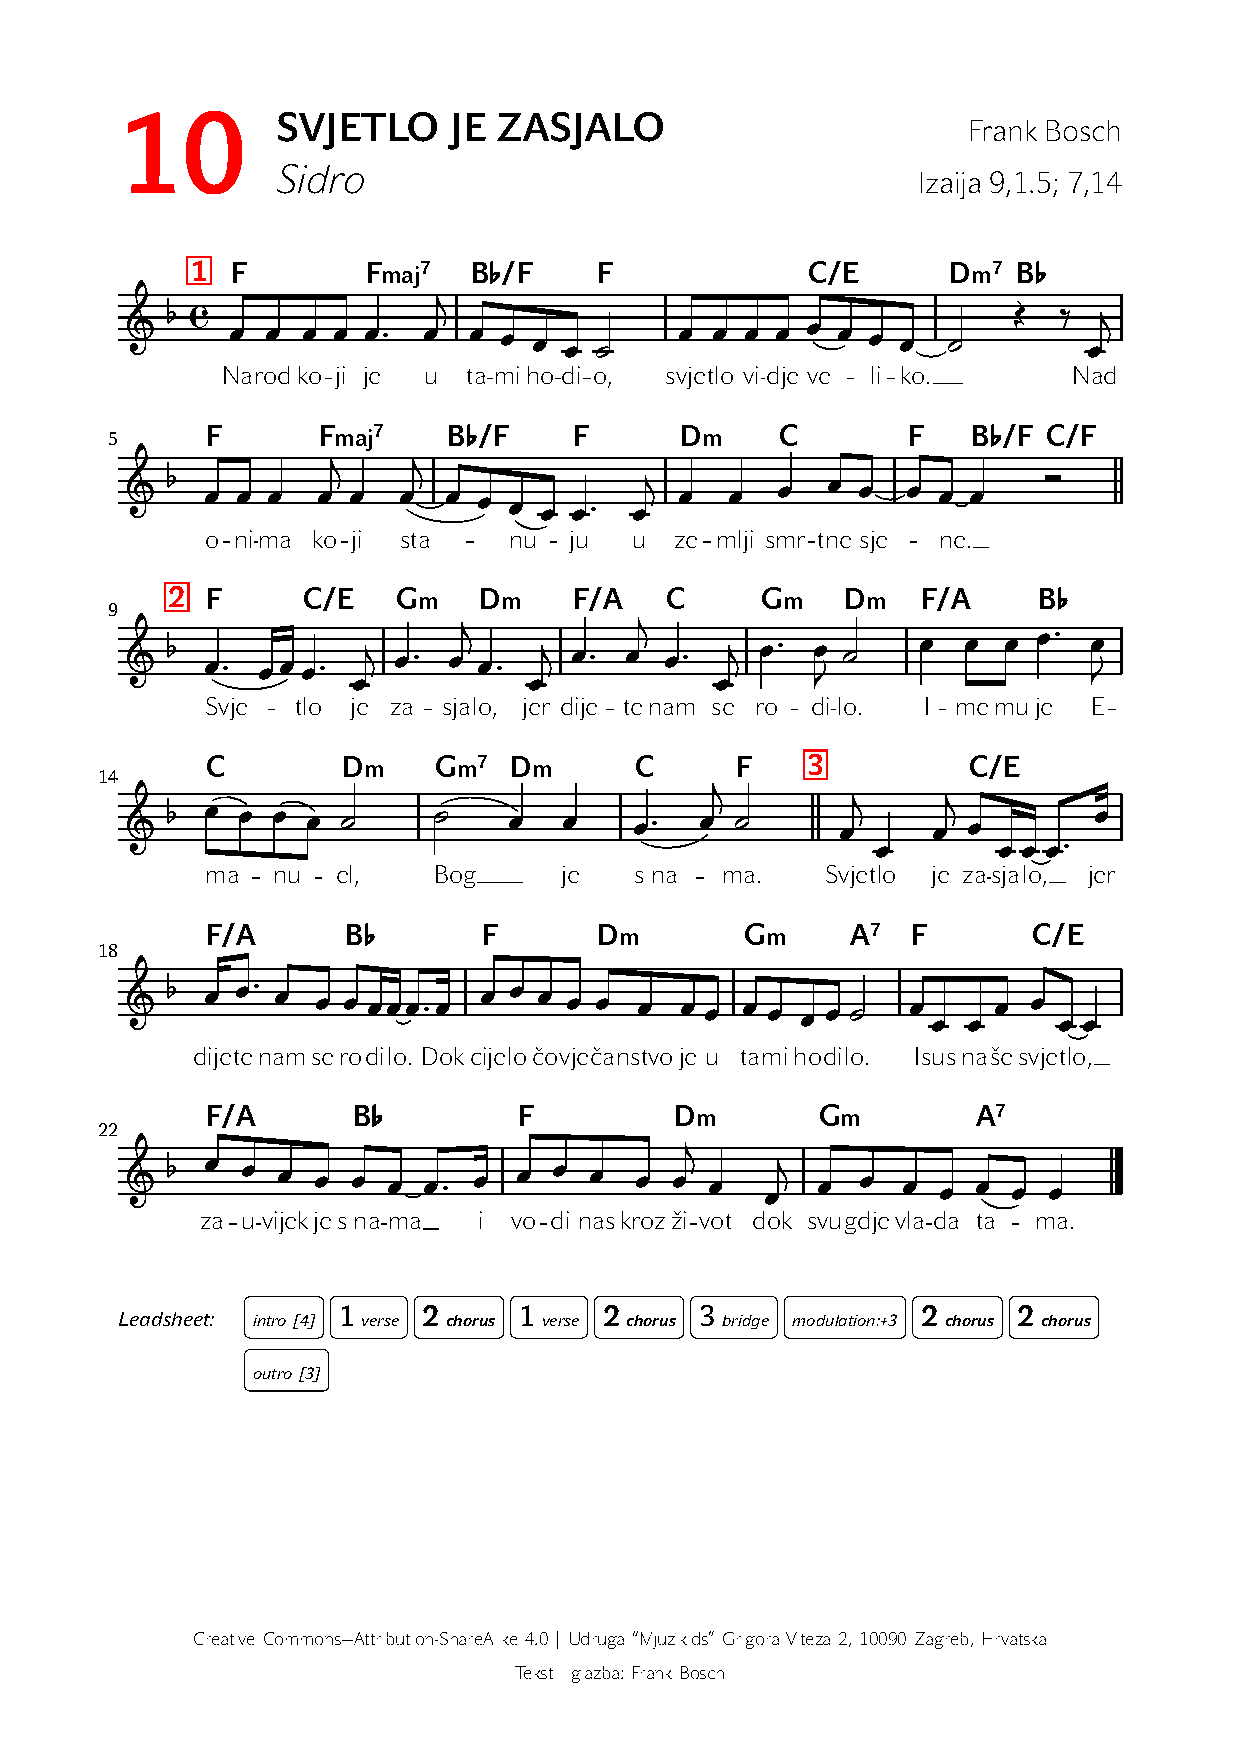
\includepdf[pages={1},noautoscale]{lilypond/hr/src/10_svjetlo_je_zasjalo.pdf}
\end{minipage}

\newpage
\begin{center}
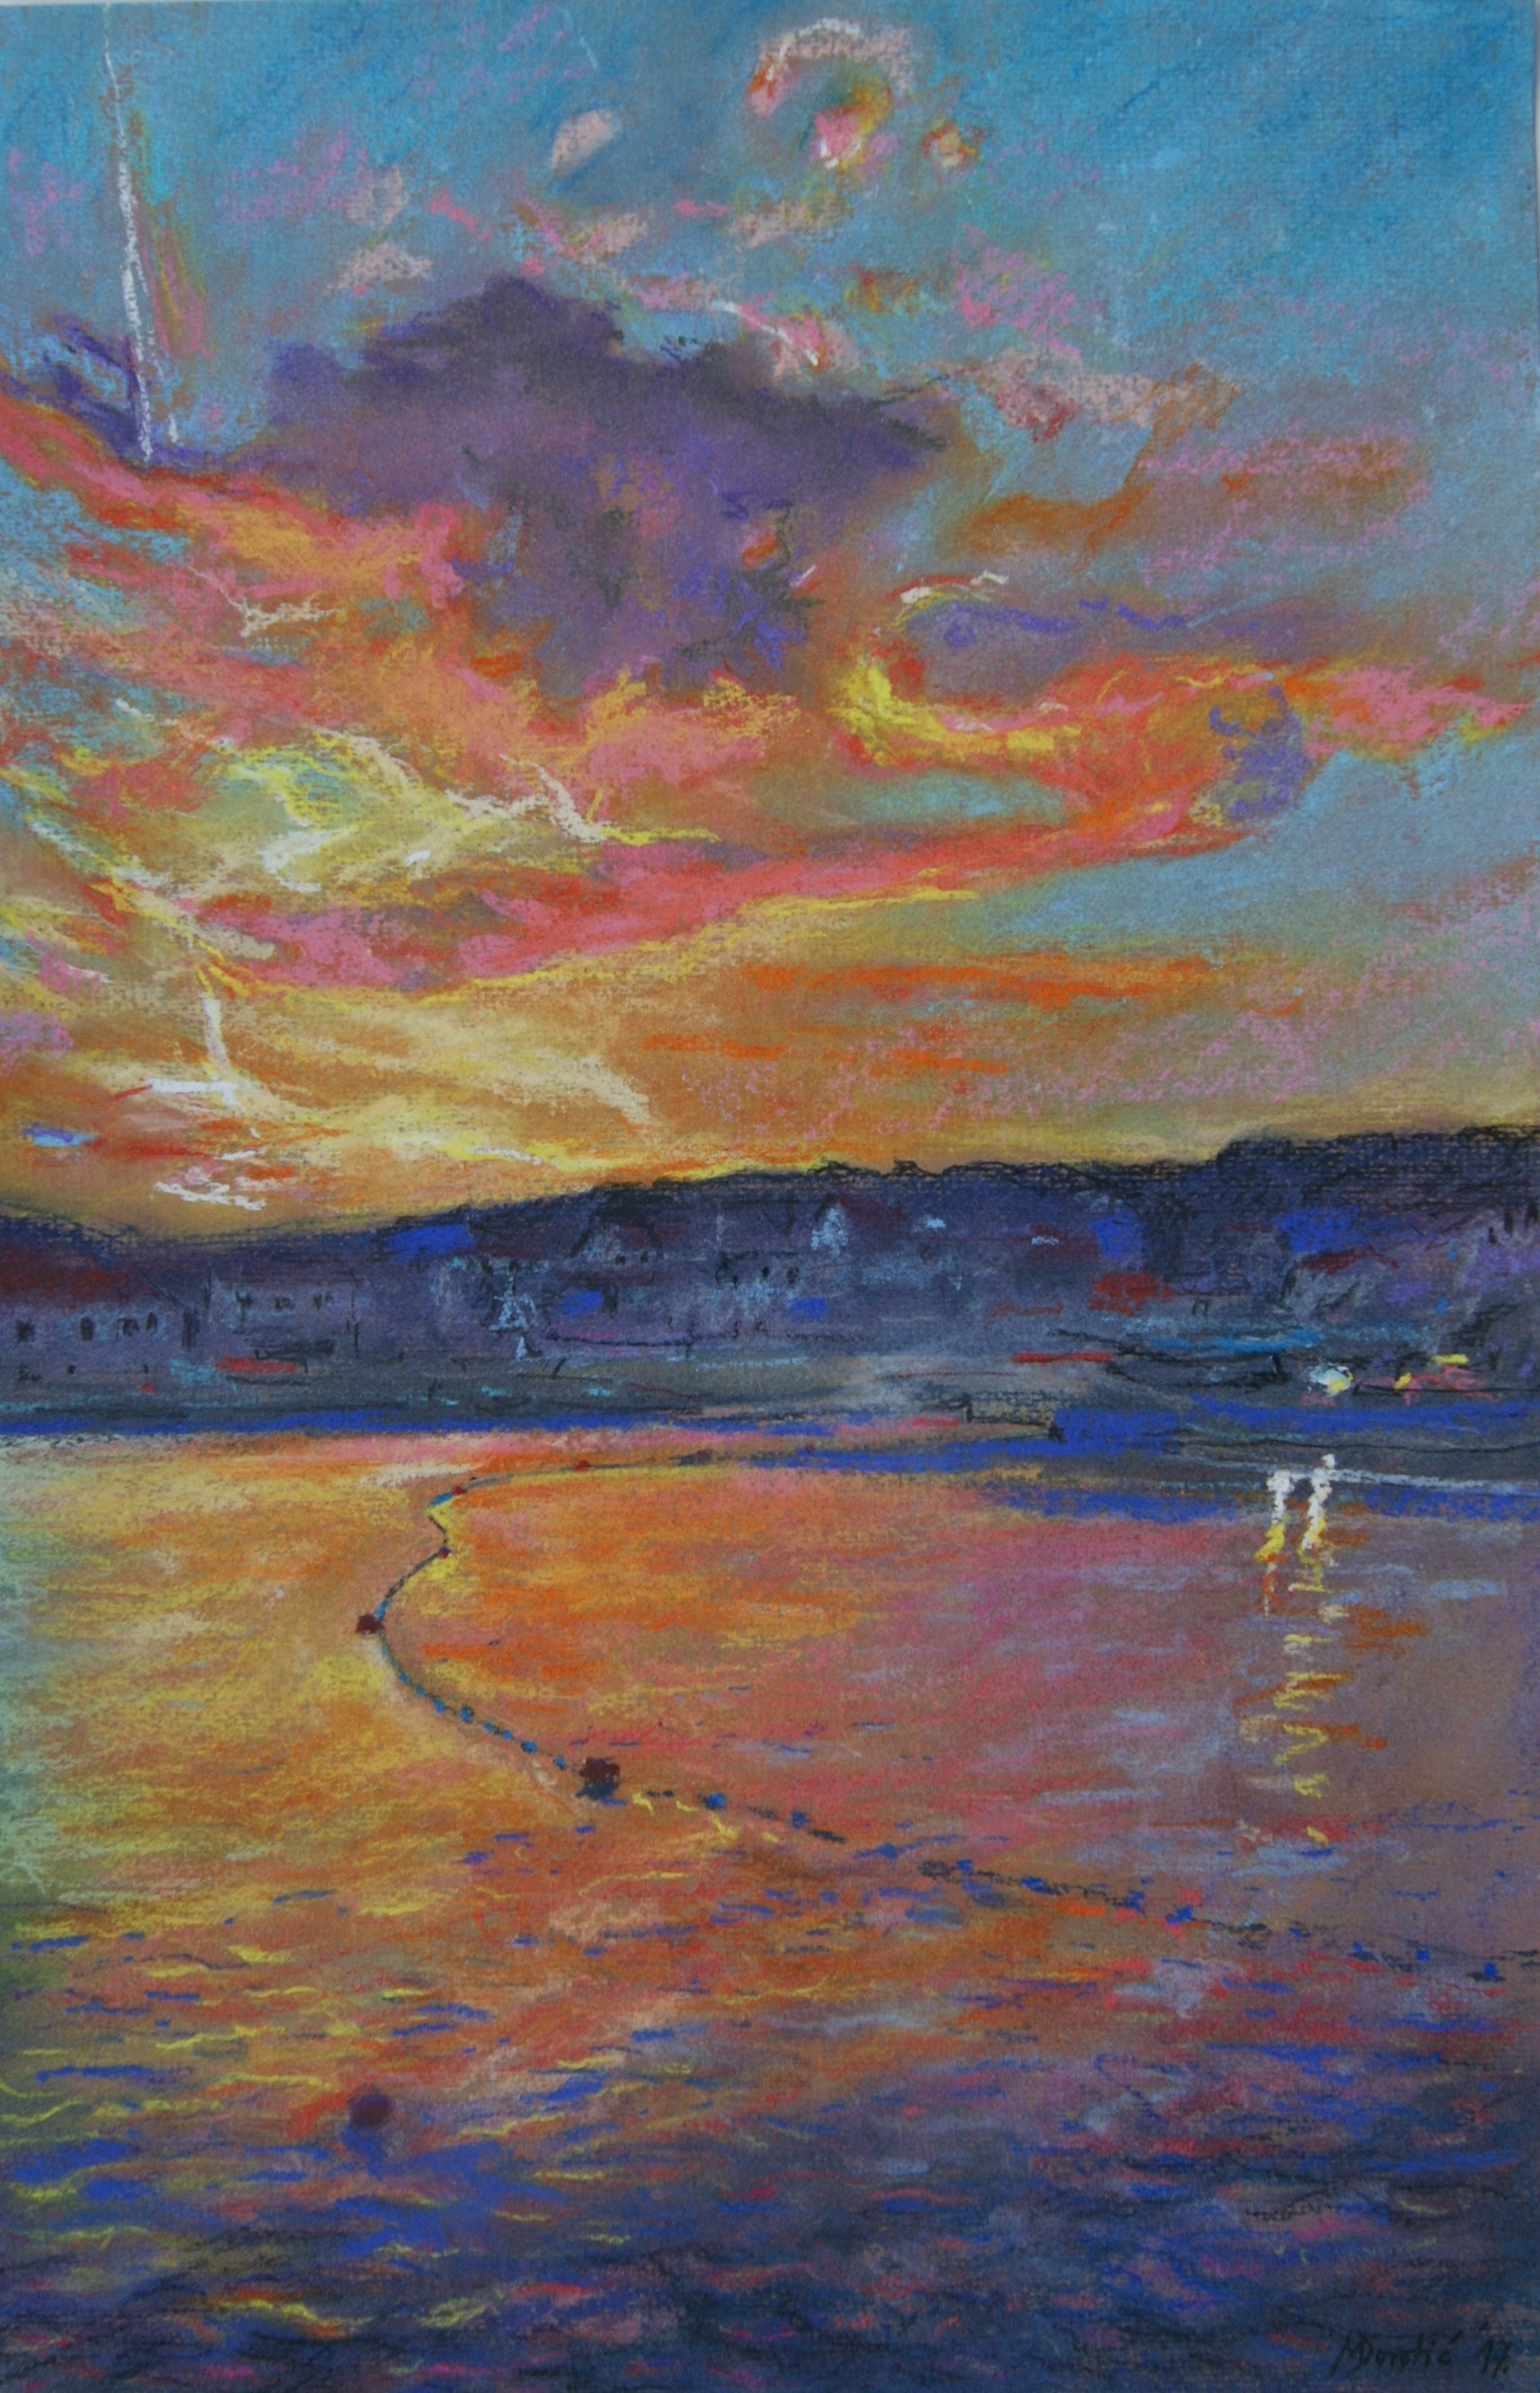
\includegraphics[width=0.9\linewidth]{images/mihovil/j10_svjetlojezasjalo}
\end{center}


%pjesma 11
\newpage
\phantomsection
\begin{minipage}[b]{0.5\linewidth}
\addcontentsline{toc}{section}{\texorpdfstring{{\rednifont\doccolor11.}\hspace{\twodigitspacing}}{}SA STABLA ŽIVOTA}
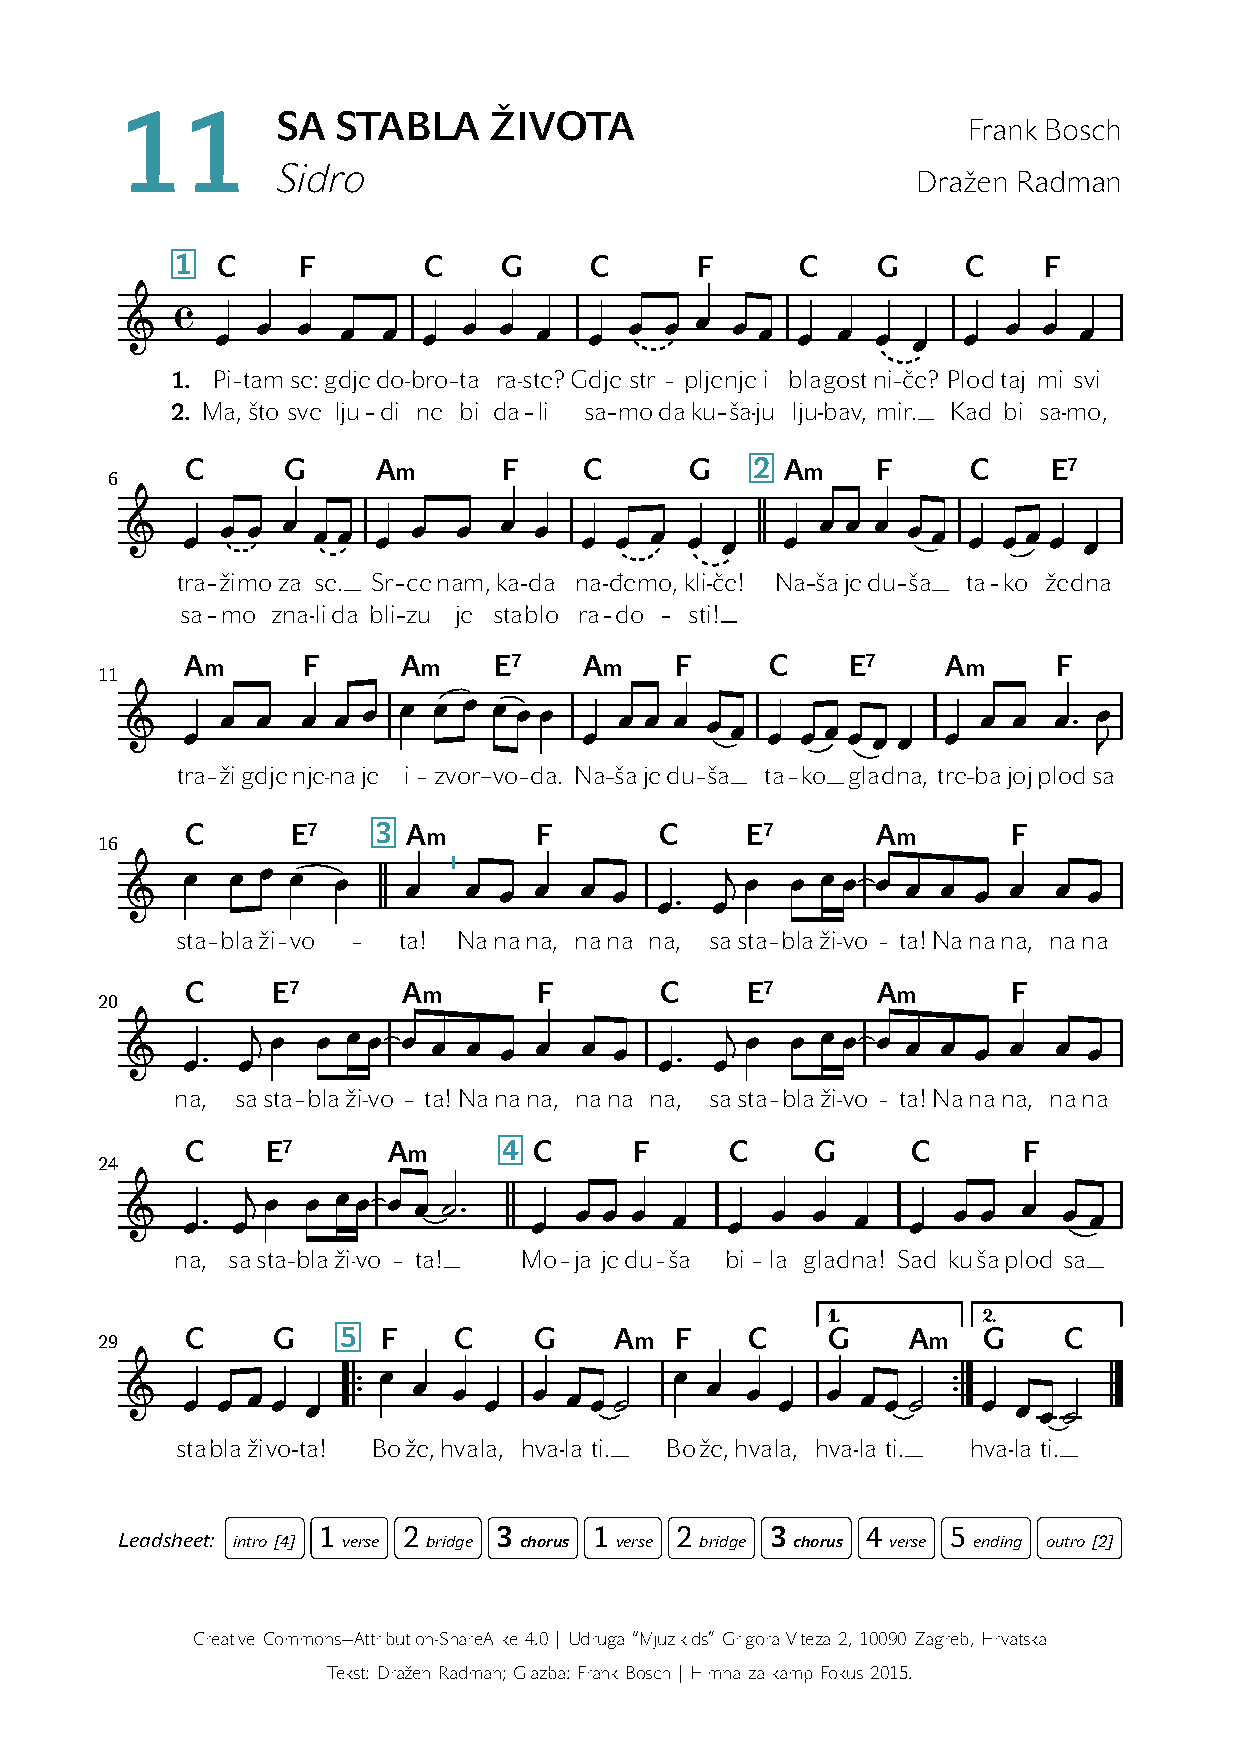
\includepdf[pages={1},noautoscale]{lilypond/hr/src/11_sa_stabla_zivota.pdf}
\end{minipage}

\newpage
\begin{center}
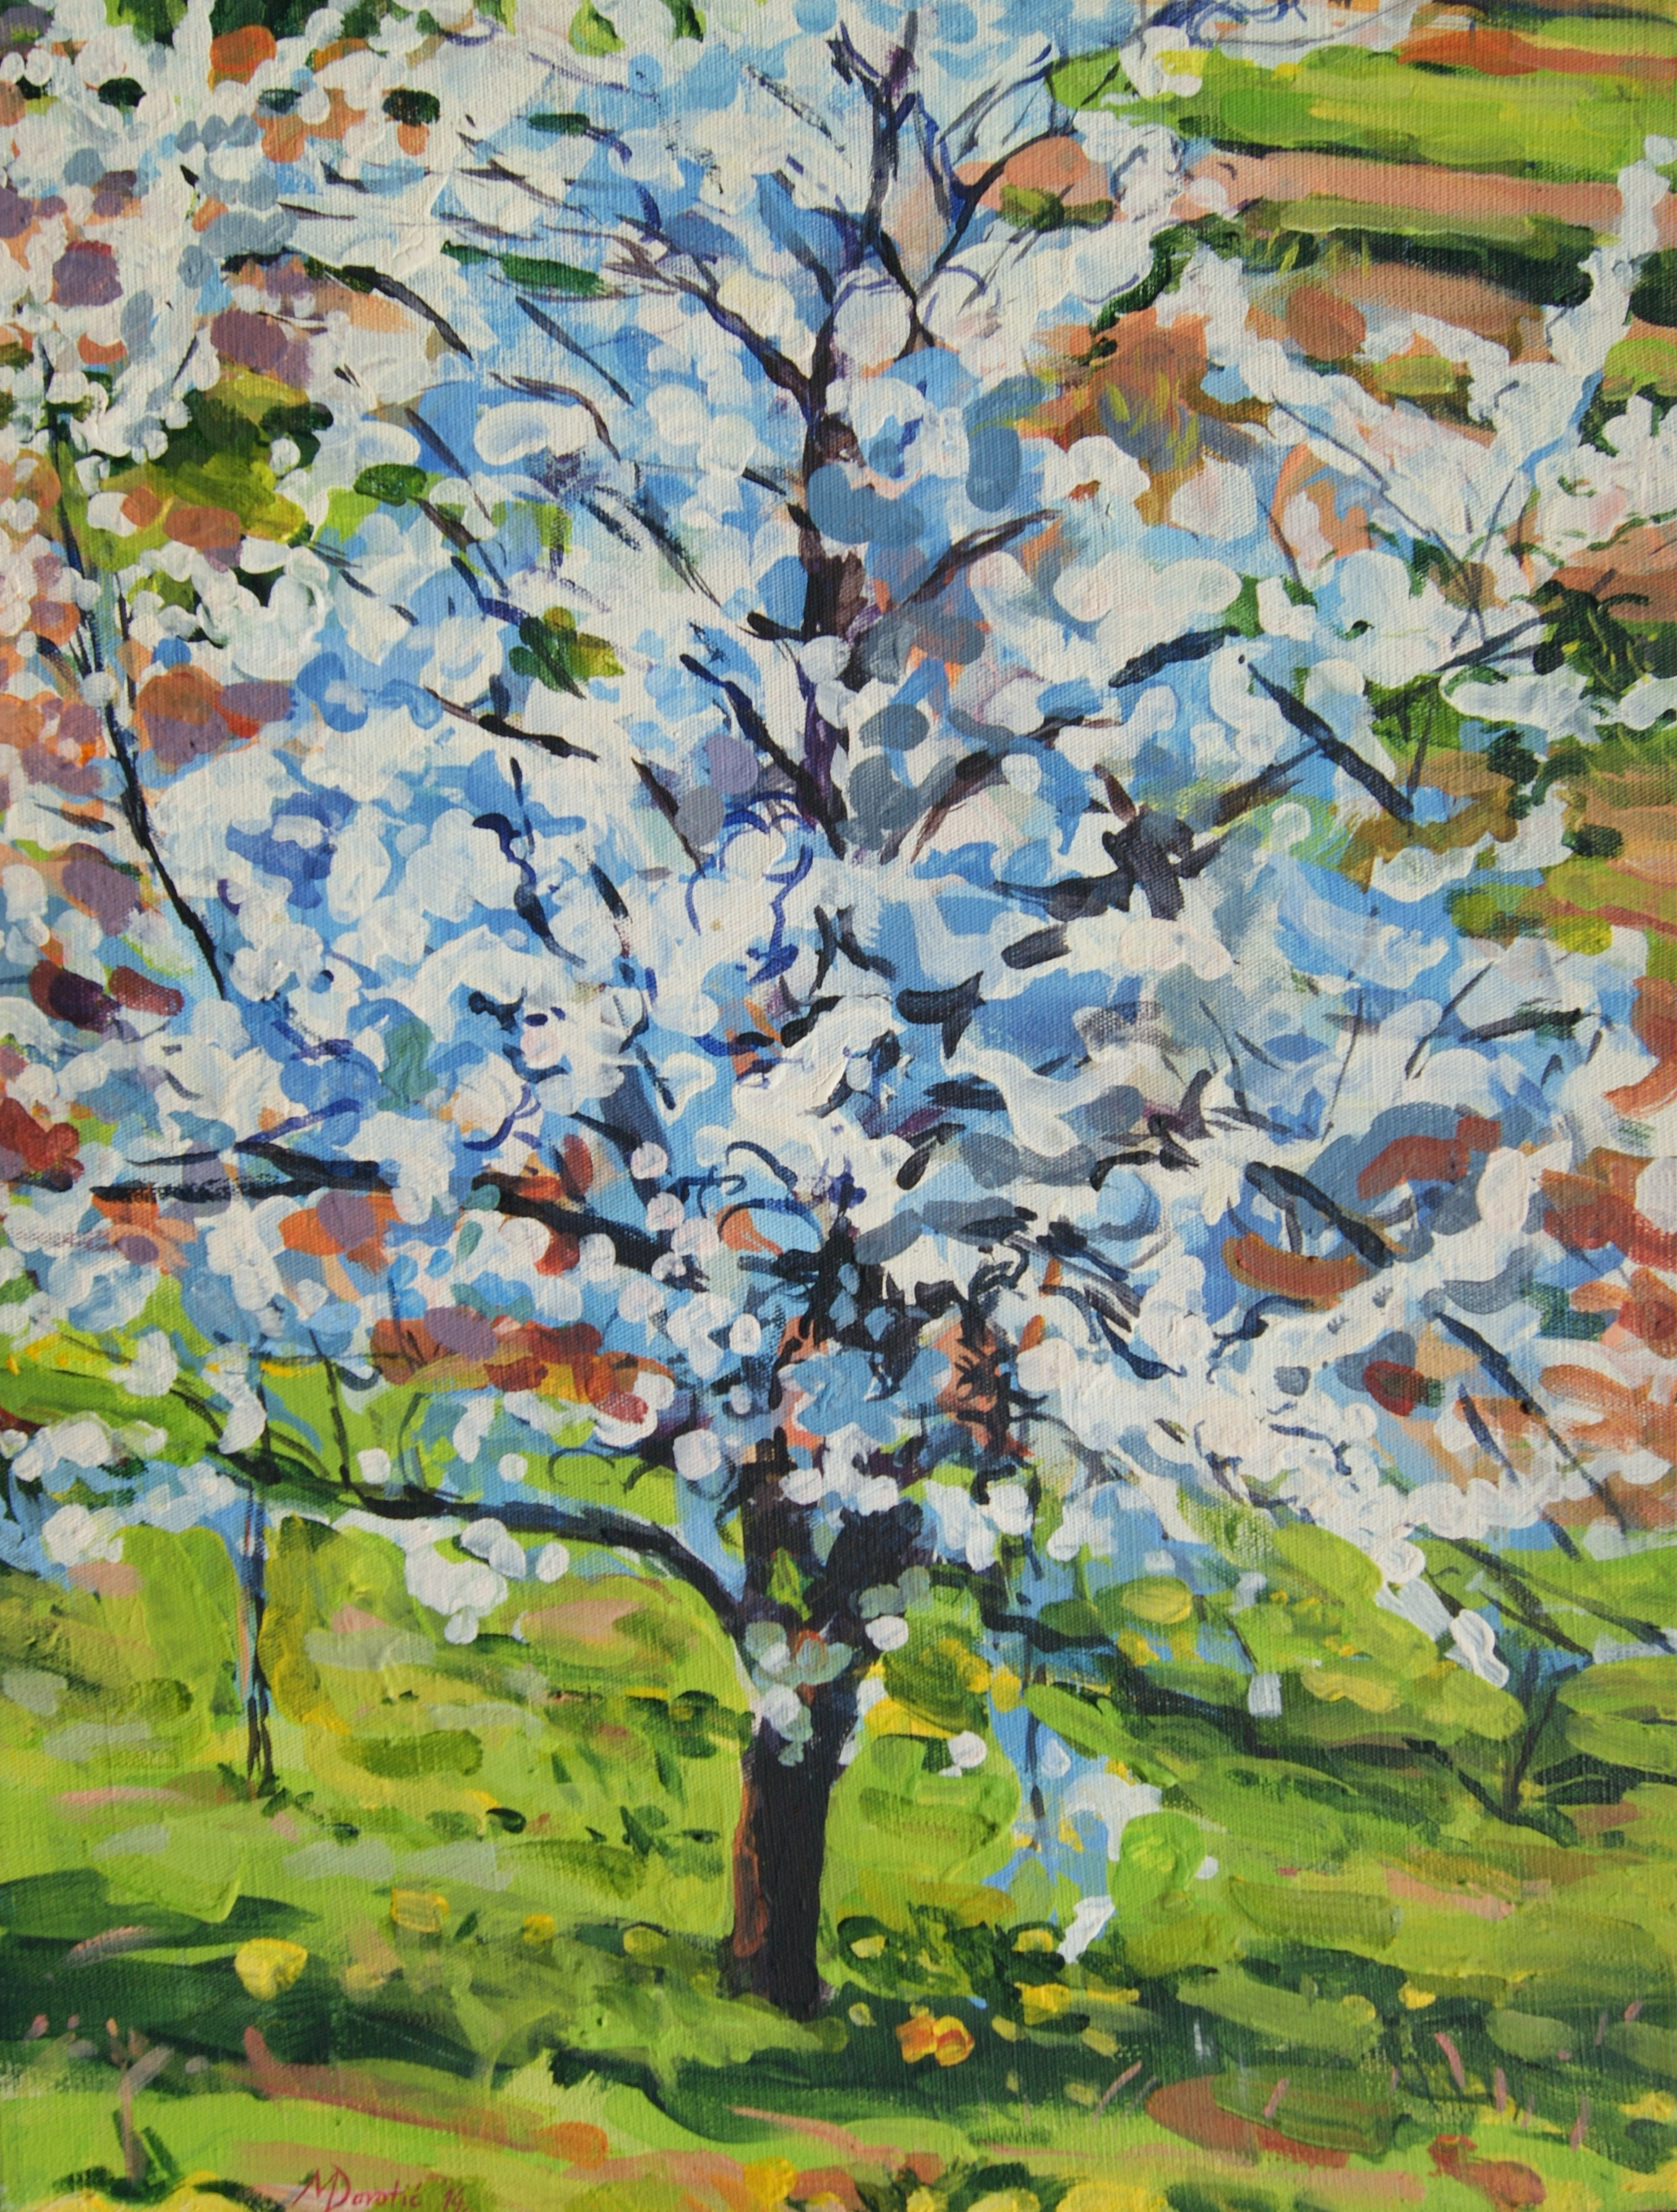
\includegraphics[width=\linewidth]{images/mihovil/k11_stablazivota}
\end{center}

%pjesma 12
\newpage
\phantomsection
\begin{minipage}[b]{0.5\linewidth}
\addcontentsline{toc}{section}{\texorpdfstring{{\rednifont\doccolor12.}\hspace{\twodigitspacing}}{}SUPER TATA \ttfamily(Rim 8,15)}
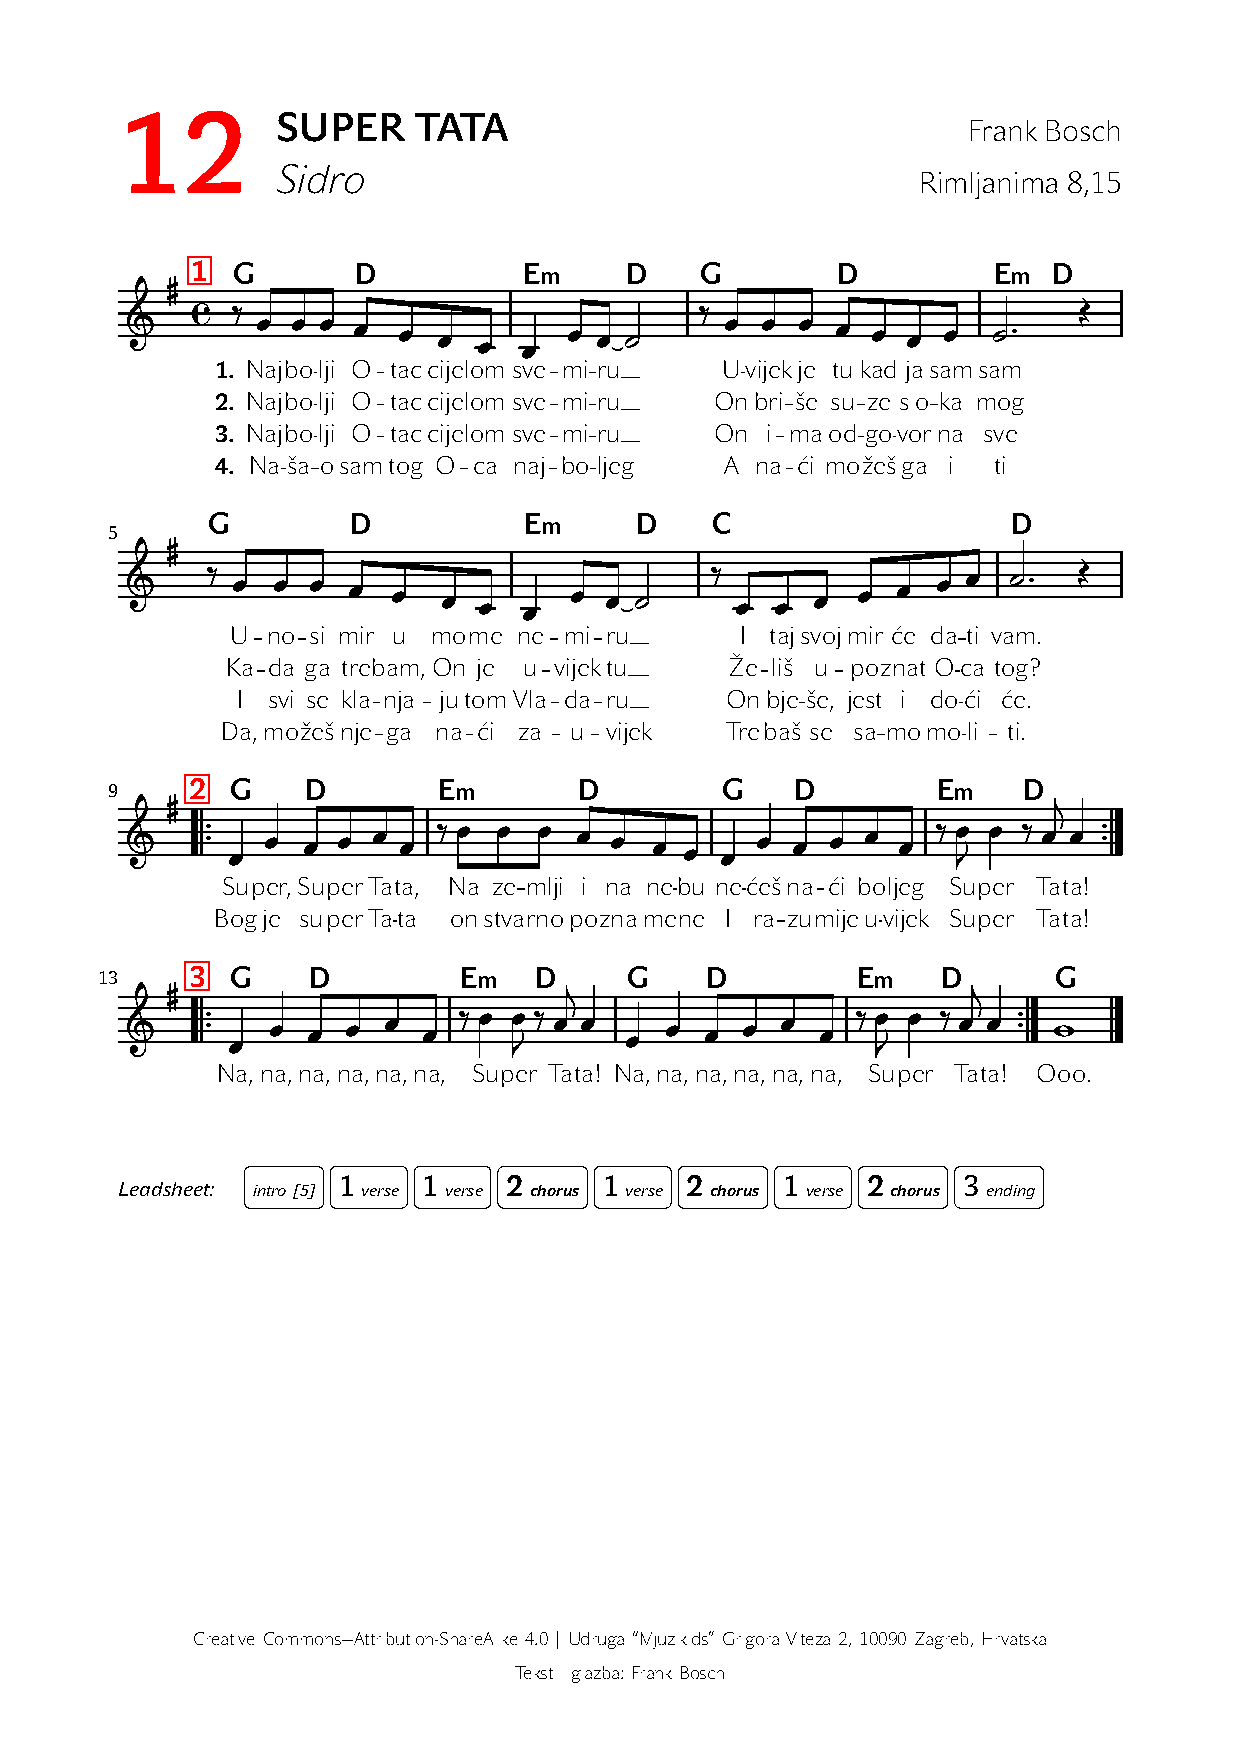
\includepdf[pages={1},noautoscale]{lilypond/hr/src/12_super_tata.pdf}
\end{minipage}

\newpage
\begin{center}
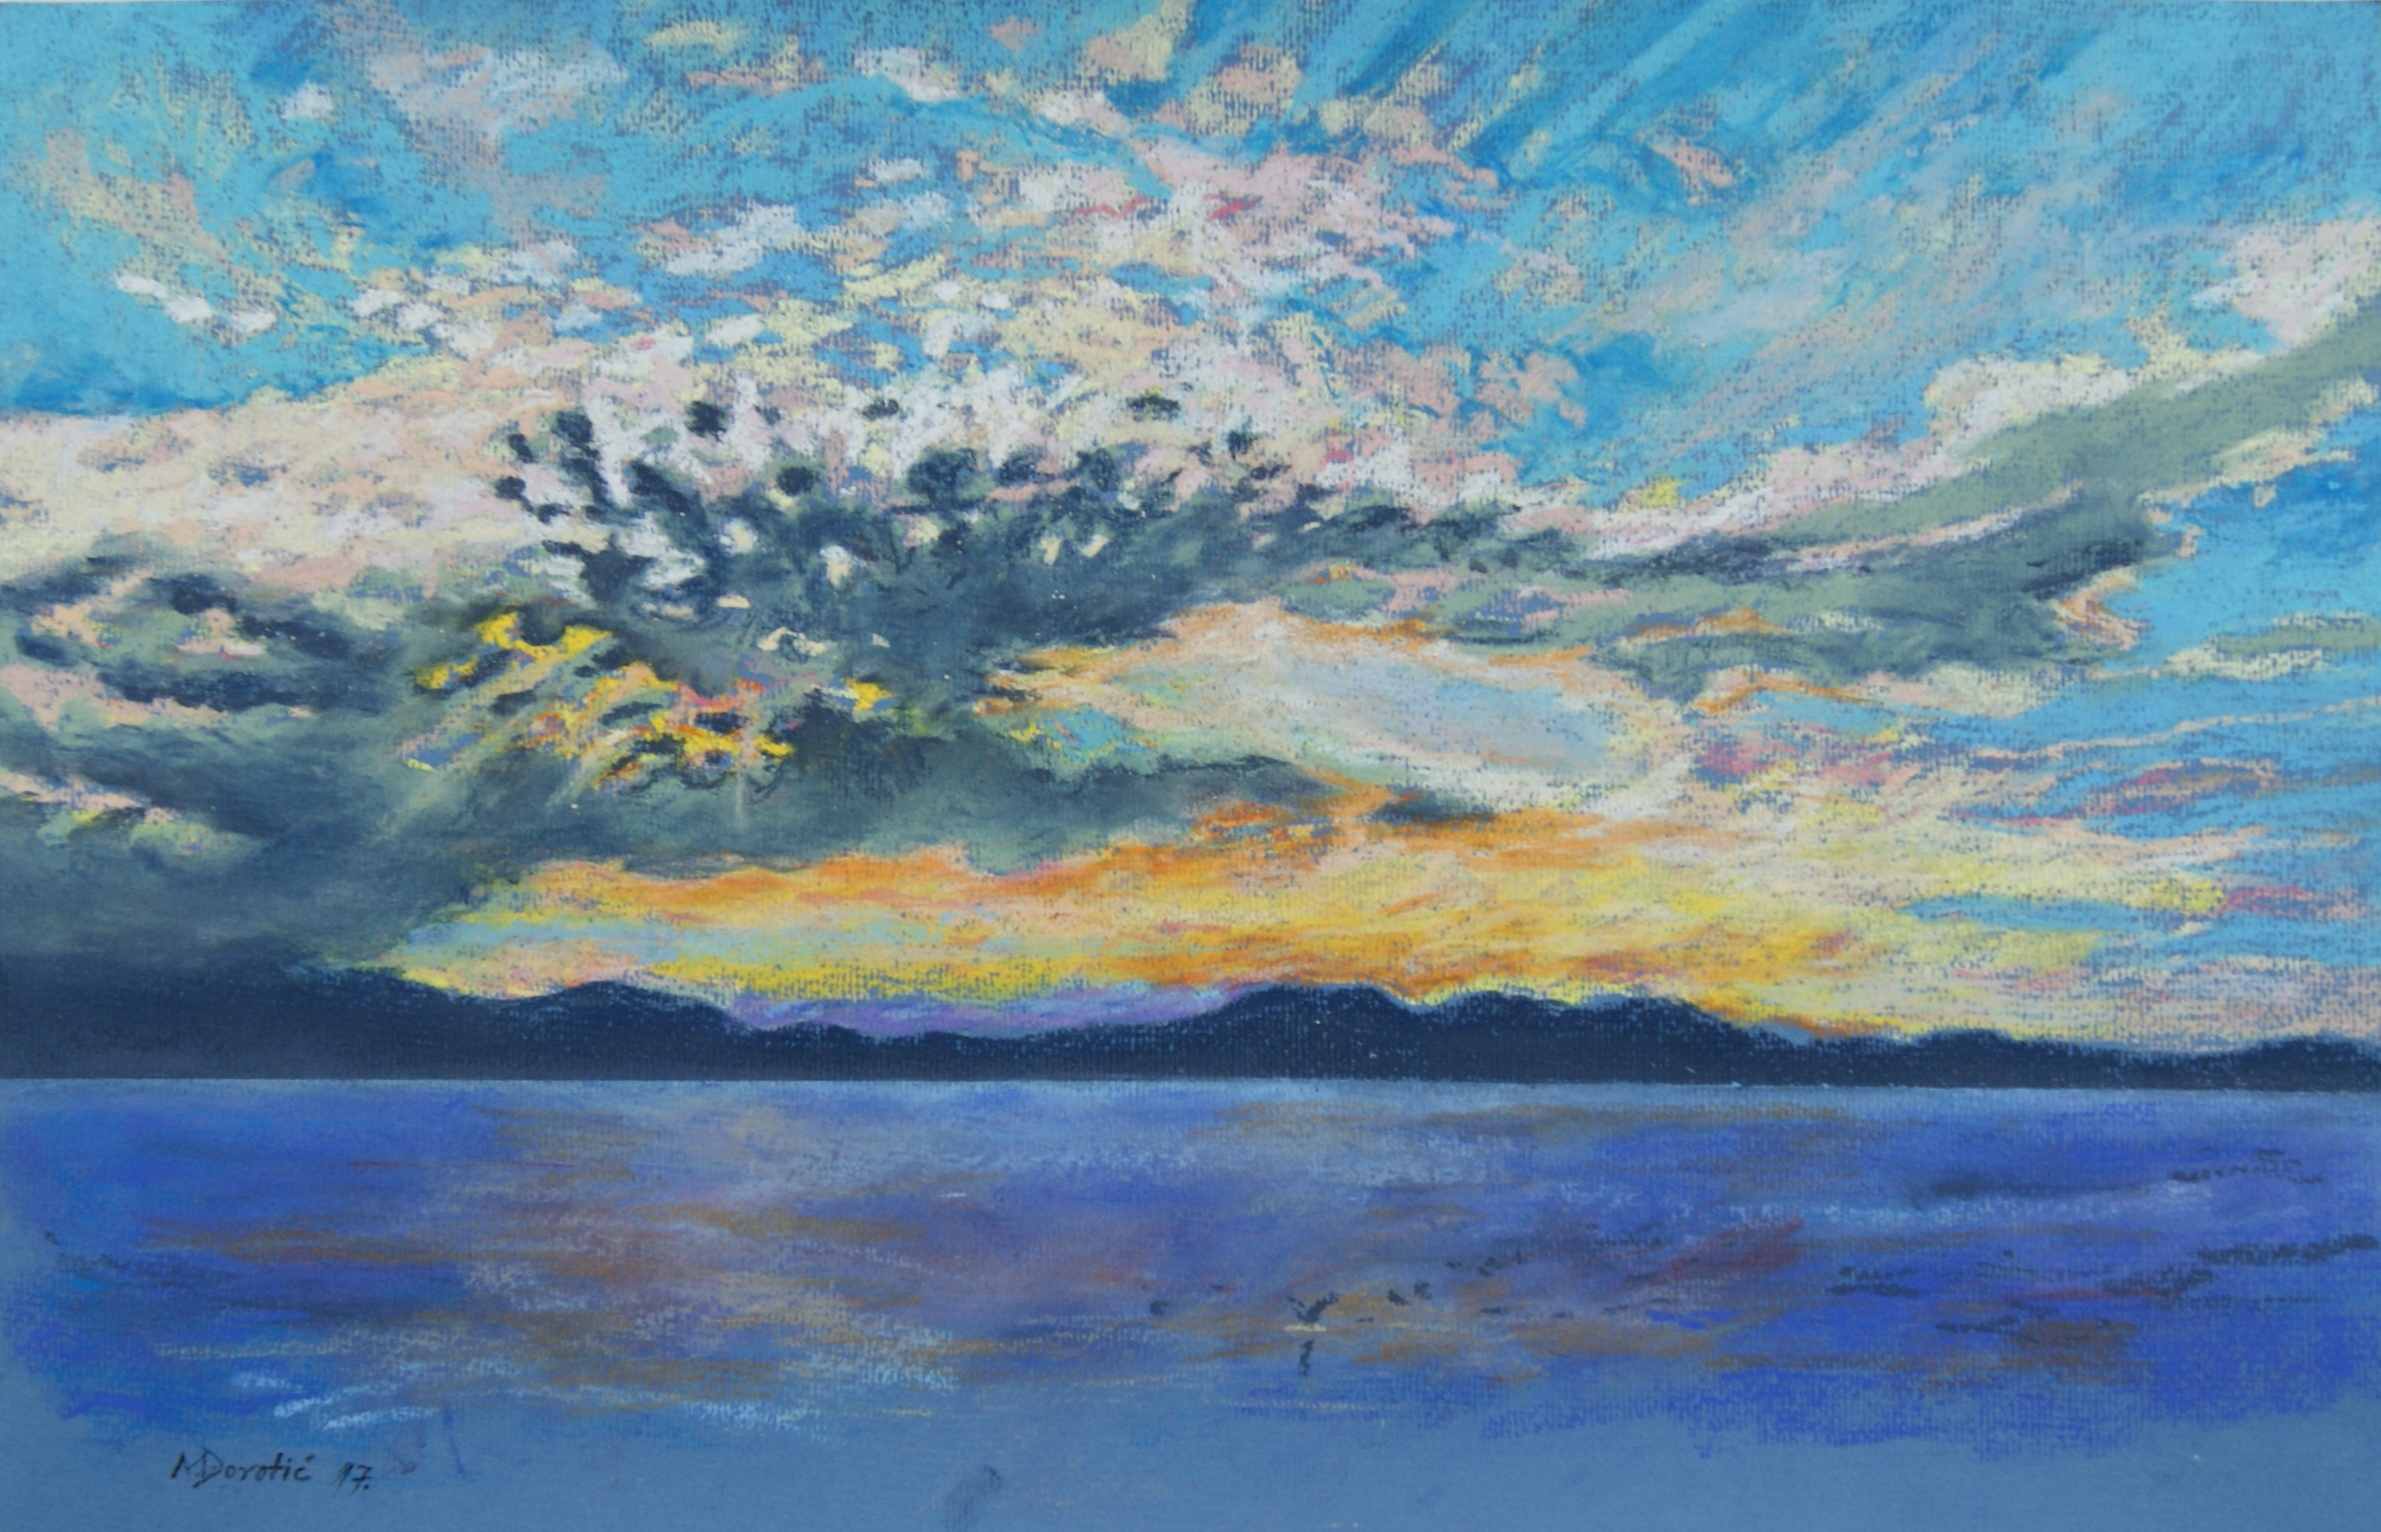
\includegraphics[width=\linewidth]{images/mihovil/l12_supertata}\\
\vspace*{1cm}
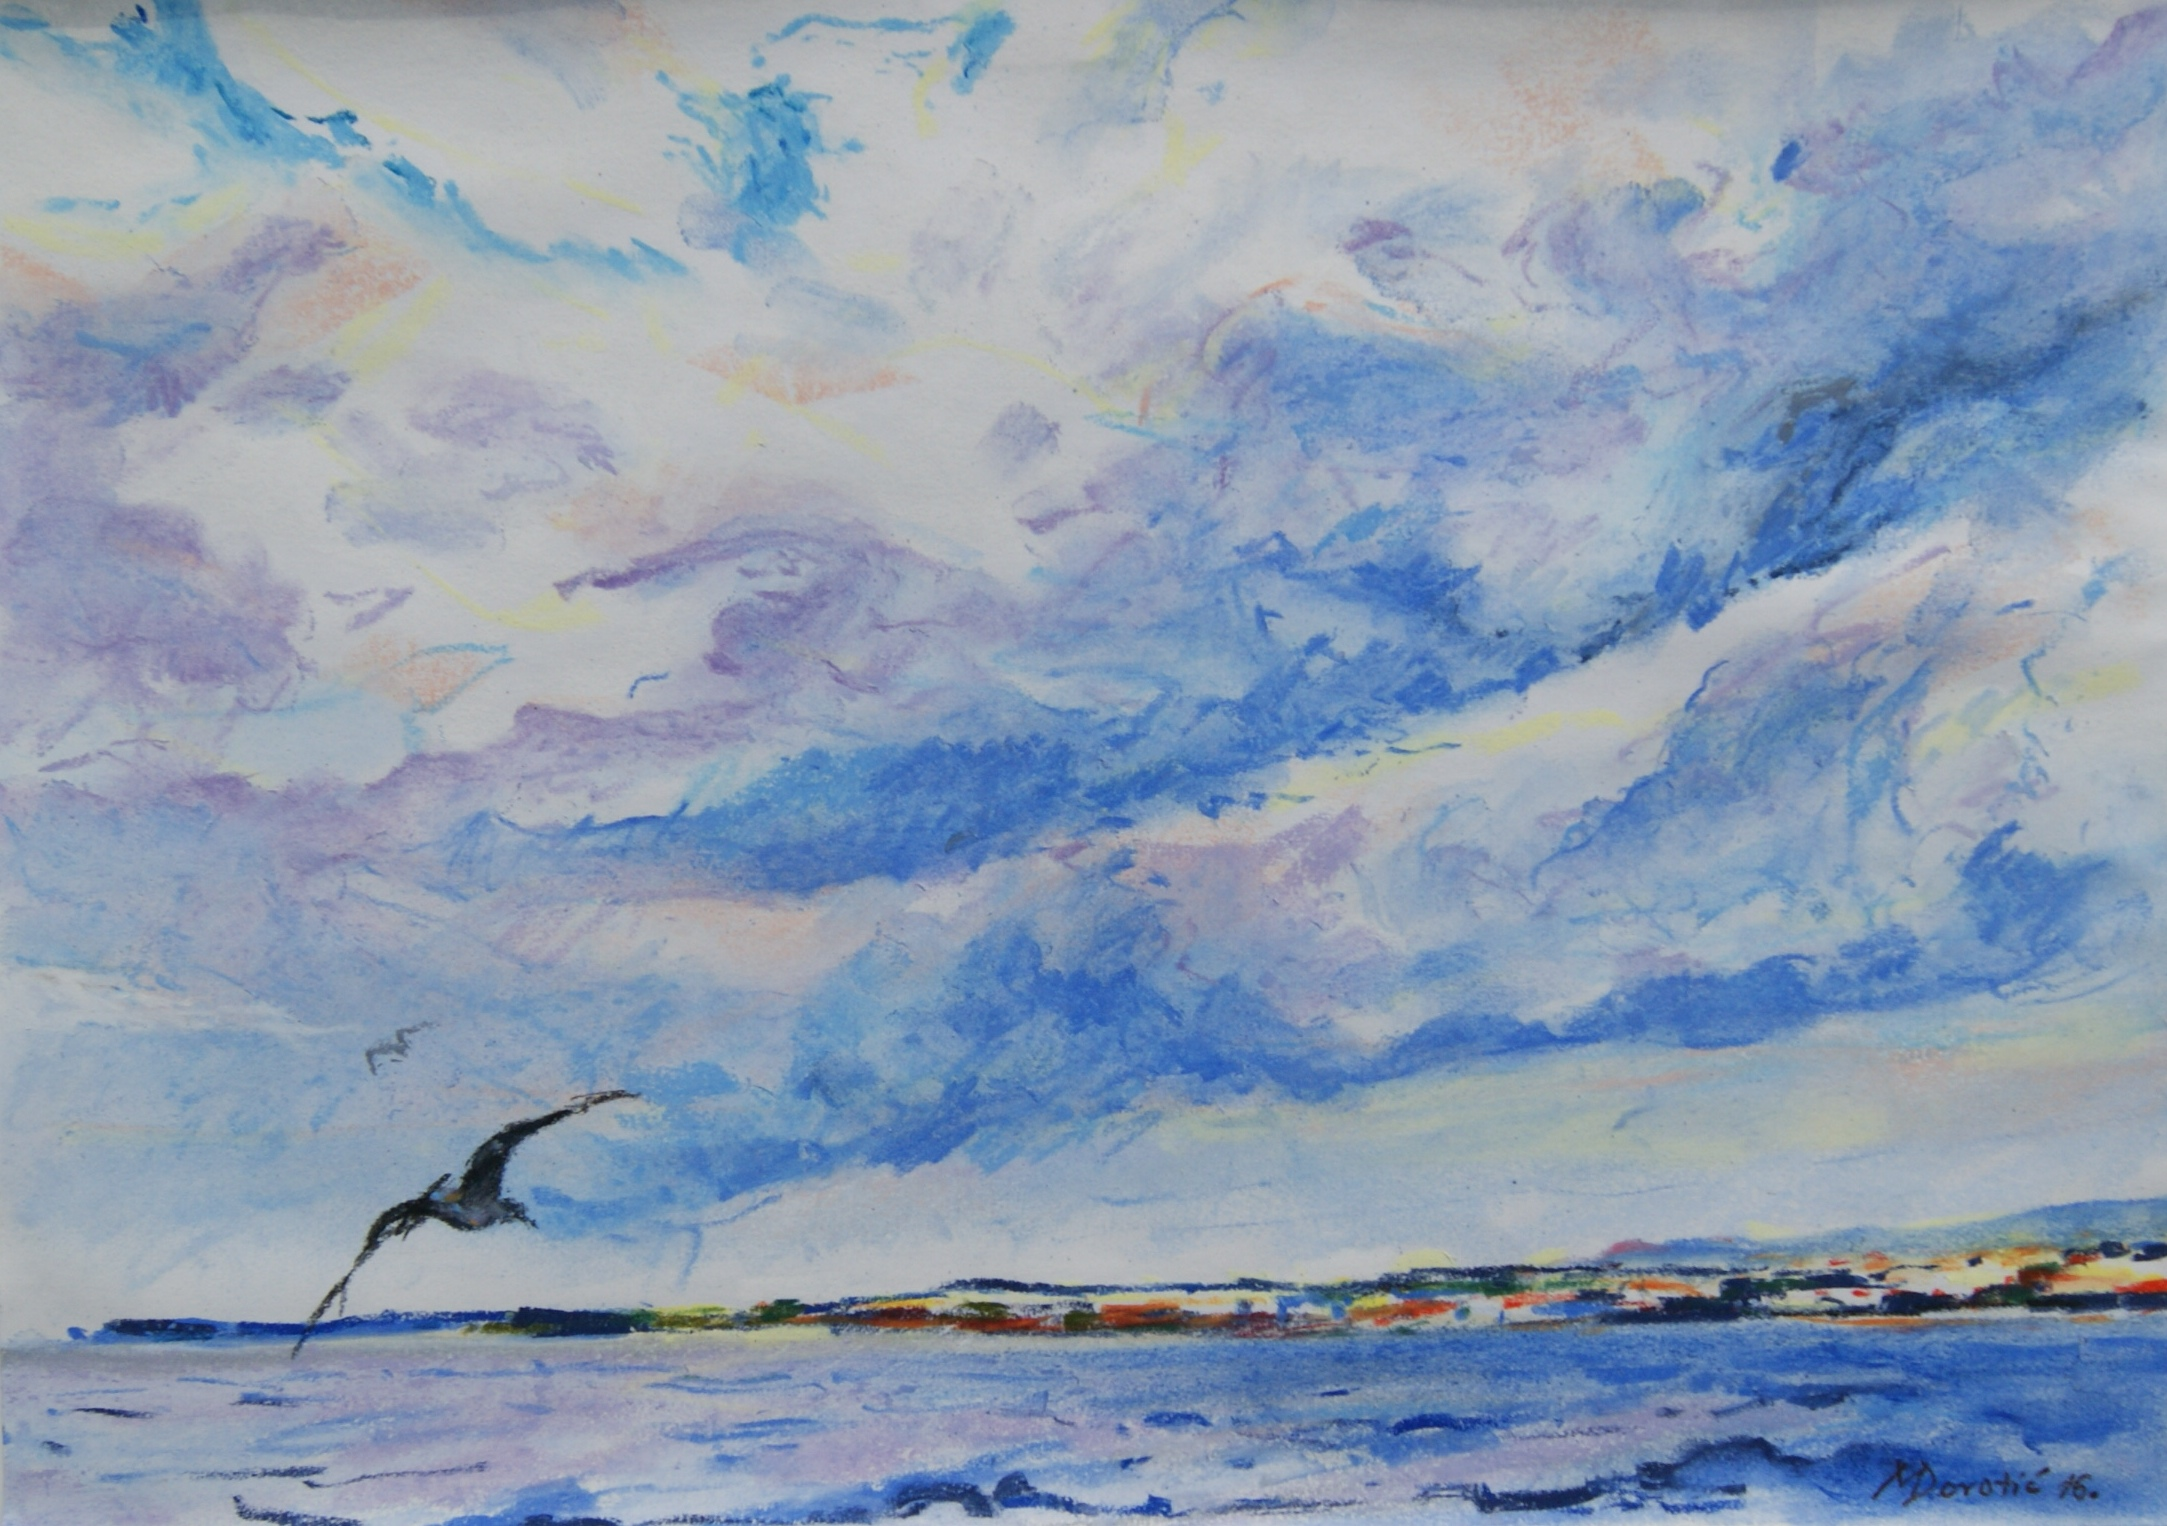
\includegraphics[width=\linewidth]{images/mihovil/m13_ubogumogu}
\end{center}

%pjesma 13
\newpage
\phantomsection
\begin{minipage}[b]{0.5\linewidth}
\addcontentsline{toc}{section}{\texorpdfstring{{\rednifont\doccolor13.}\hspace{\twodigitspacing}}{}U BOGU MOGU}
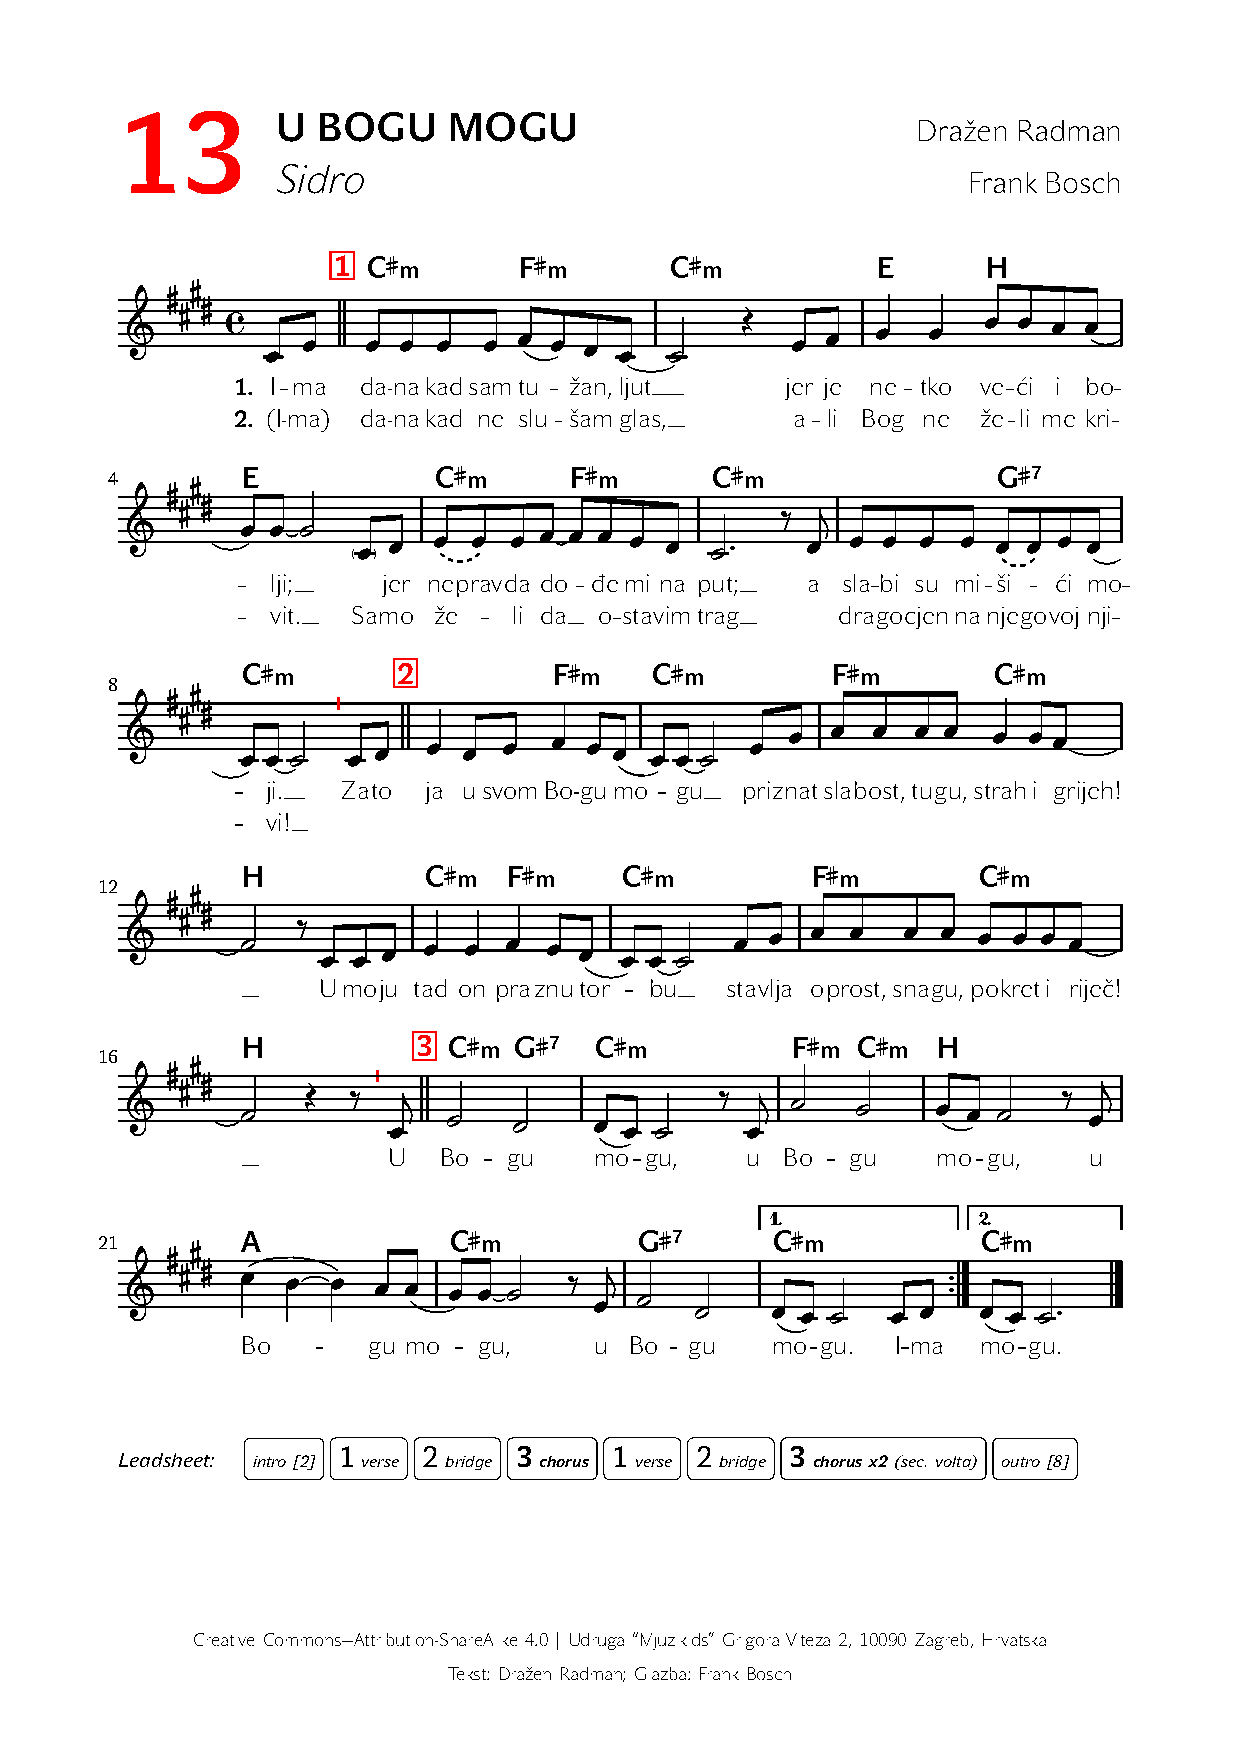
\includepdf[pages={1},noautoscale]{lilypond/hr/src/13_u_bogu_mogu.pdf}
\end{minipage}

\newpage
\begin{center}
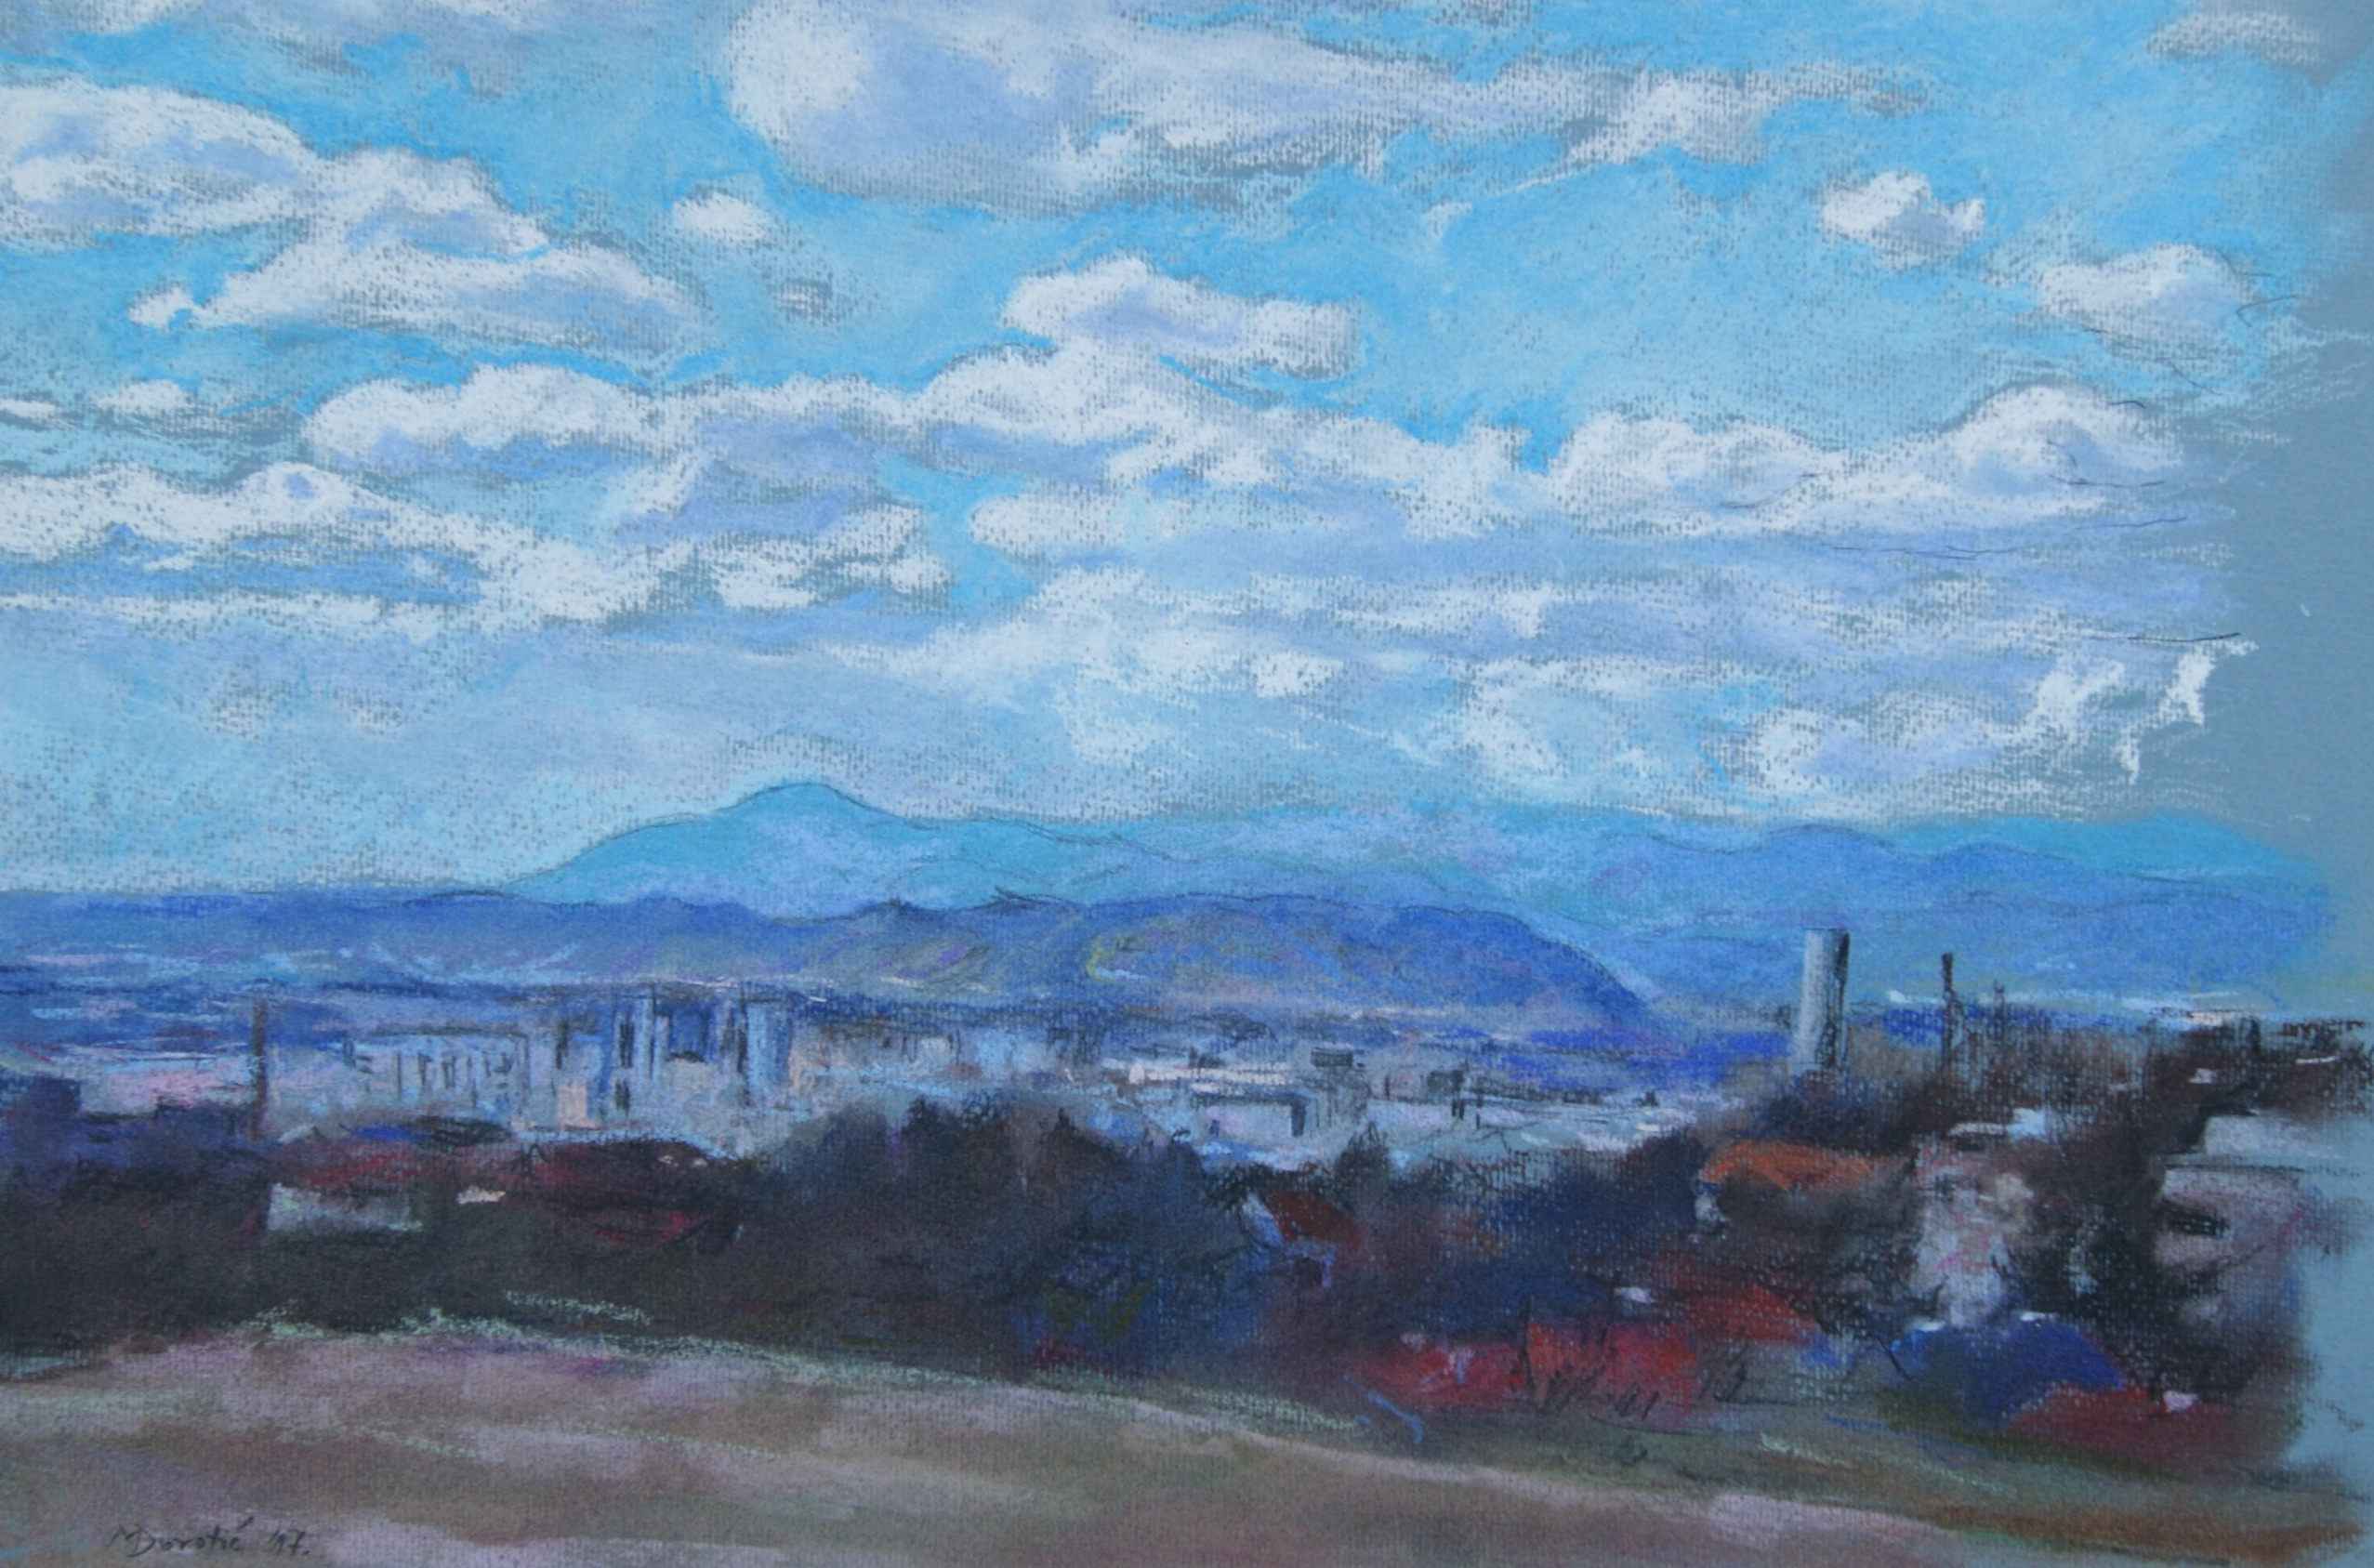
\includegraphics[width=\linewidth]{images/mihovil/c3_planovemira}

\vspace*{1mm}
\begin{center}

	\Large{\parbox{\linewidth}{
		\begin{center}
		{\Large
		\texttt{
			\textit{"'Jer ja znam svoje naume koje s vama namjeravam' – riječ je Jahvina – 'naume mira, a ne nesreće: da vam dadnem budućnost i nadu.'"}
			}
		}
		\end{center}
		\begin{center}
		{\Large
			\texttt{{\textemdash Jeremija 29,11}}
		}
		\end{center}
	}
}
\end{center}

\end{center}

% \newpage
% \thispagestyle{empty}%
% \vspace*{10.5cm}
% \begin{center}
% Ova je stranica namjerno ostavljena prazna.\\
% Diese Seite wurde mit Absicht leer gelassen.
% \end{center}

\vfill

%=========================================
%   DISKOGRAFIJA
%=========================================
%zadnje tri strane - prema Frankovoj želji - fake rekonstrukcija pdfova sa slikama koje ne idu od  ruba do ruba
\newpage

\section*{MJUZIKIDS DISKOGRAFIJA / MJUZIKIDS DISKOGRAPHIE}

\begin{center}
\vspace{1cm}
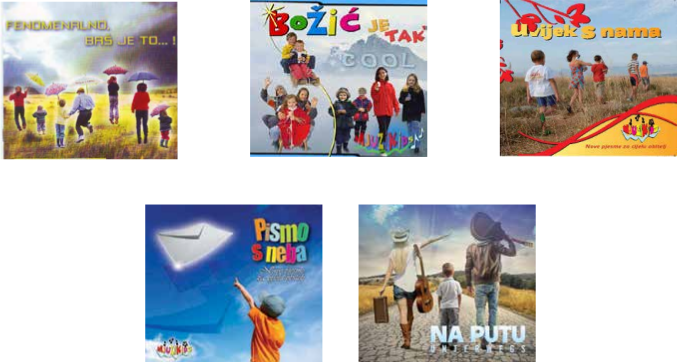
\includegraphics[width=\linewidth]{images/cd}

\vspace{1cm}
Javite se ako ste zainteresirani da skupina Mjuzikids održi koncert kod vas,
ako želite naručiti pjesmarice ili neke od naših prijašnjih CDa.\\
\vspace{1cm}
Melden Sie sich, wenn Sie Interesse an einem Auftritt von Frank Bosch haben oder
wenn Sie unsere früheren CDs bzw. Liederbücher bestellen möchten.
\vfill
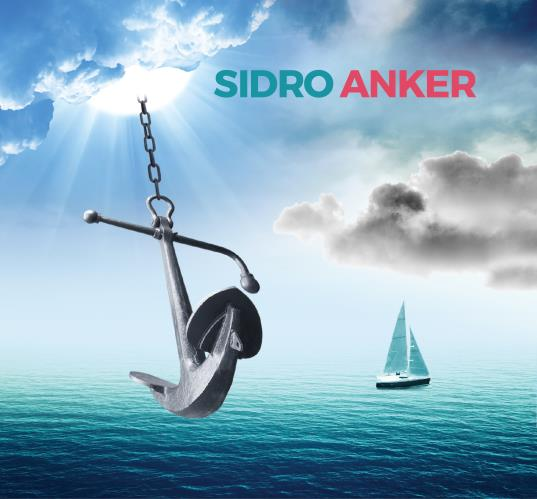
\includegraphics[width=0.5\linewidth]{images/Sidro_cd}
\vfill

\end{center}

%=========================================
%   SURADNICI I DRAGI PRIJATELJI
%=========================================
\newpage

\section*{SURADNICI I DRAGI PRIJATELJI /\\ UNSERE MITARBEITER UND LIEBE FREUNDE}
\begin{center}
\vspace{1cm}
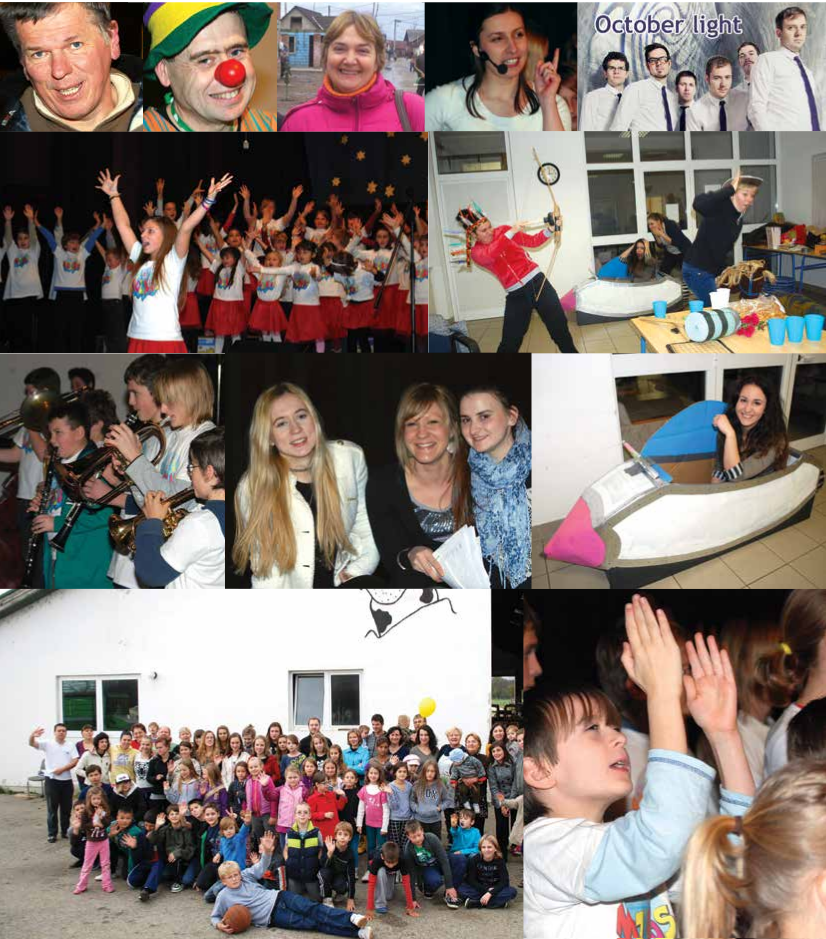
\includegraphics[width=1\linewidth]{images/suradnici}\\
\end{center}



\end{document}
%#################################################################################
%   END OF DOCUMENT
%#################################################################################